%%%%%%%%%%%%%%%%%%%%%%%%%%%%%%%%%%%%%%%%%
% Masters/Doctoral Thesis 
% LaTeX Template
% Version 1.43 (17/5/14)
%
% This template has been downloaded from:
% http://www.LaTeXTemplates.com
%
% Original authors:
% Steven Gunn 
% http://users.ecs.soton.ac.uk/srg/softwaretools/document/templates/
% and
% Sunil Patel
% http://www.sunilpatel.co.uk/thesis-template/
%
% License:
% CC BY-NC-SA 3.0 (http://creativecommons.org/licenses/by-nc-sa/3.0/)
%
% Note:
% Make sure to edit document variables in the Thesis.cls file
%
%%%%%%%%%%%%%%%%%%%%%%%%%%%%%%%%%%%%%%%%%

%----------------------------------------------------------------------------------------
%	PACKAGES AND OTHER DOCUMENT CONFIGURATIONS
%----------------------------------------------------------------------------------------

\documentclass[11pt, oneside]{Thesis} % The default font size and one-sided printing (no margin offsets)

\graphicspath{{Pictures/}} % Specifies the directory where pictures are stored
\usepackage{wrapfig}
\usepackage{graphicx}
\usepackage{caption}
\usepackage{subcaption}
\usepackage{amsmath}

\usepackage[square, numbers, comma, sort&compress]{natbib} % Use the natbib reference package - read up on this to edit the reference style; if you want text (e.g. Smith et al., 2012) for the in-text references (instead of numbers), remove 'numbers' 
\hypersetup{urlcolor=blue, colorlinks=true} % Colors hyperlinks in blue - change to black if annoying
\title{\ttitle} % Defines the thesis title - don't touch this

\begin{document}

\frontmatter % Use roman page numbering style (i, ii, iii, iv...) for the pre-content pages

\setstretch{1.1} % Line spacing of 1.3

% Define the page headers using the FancyHdr package and set up for one-sided printing
\fancyhead{} % Clears all page headers and footers
\rhead{\thepage} % Sets the right side header to show the page number
\lhead{} % Clears the left side page header

\pagestyle{fancy} % Finally, use the "fancy" page style to implement the FancyHdr headers

\newcommand{\HRule}{\rule{\linewidth}{0.5mm}} % New command to make the lines in the title page

% PDF meta-data
\hypersetup{pdftitle={\ttitle}}
\hypersetup{pdfsubject=\subjectname}
\hypersetup{pdfauthor=\authornames}
\hypersetup{pdfkeywords=\keywordnames}

%----------------------------------------------------------------------------------------
%	TITLE PAGE
%----------------------------------------------------------------------------------------

\begin{titlepage}
\begin{center}

\textsc{\LARGE Imperial College London}\\[1.5cm] % University name
\textsc{\Large Department of Computing}\\[0.5cm] % Thesis type

\HRule \\[0.4cm] % Horizontal line
{\huge \bfseries Turning Music Into Game}\\[0.4cm] % Thesis title
\HRule \\[1.5cm] % Horizontal line
 
\begin{minipage}{0.4\textwidth}
\begin{flushleft} \large
\emph{Author:}\\
\href{pak11@doc.ic.ac.uk}{Paulina Koch} % Author name - remove the \href bracket to remove the link
\end{flushleft}
\end{minipage}
\begin{minipage}{0.4\textwidth}
\begin{flushright} \large
\emph{Supervisor:} \\
Dr. Iain Phillips \\ \vspace{20pt}
\emph{2nd Marker:} \\
Dr. Robert Chatley
\end{flushright}
\end{minipage}\\[3cm]
 

{\large \today}\\[4cm] % Date
%\includegraphics{Logo} % University/department logo - uncomment to place it
 
\vfill
\end{center}

\end{titlepage}


%----------------------------------------------------------------------------------------
%	THESIS CONTENT - CHAPTERS
%----------------------------------------------------------------------------------------
\mainmatter
% Chapter Template

\chapter{Abstract} % Main chapter title

\label{Abstract} % Change X to a consecutive number; for referencing this chapter elsewhere, use \ref{ChapterX}

\lhead{Abstract} % Change X to a consecutive number; this is for the header on each page - perhaps a shortened title

Music games present a highly pervasive new platform to create, perform and appreciate music. In case of music rhythm games, very often the player is limited to the songs preprocessed by the game developers. In this project we attempt to create a music rhythm game which, given a music track, extracts its features to generate a level without human intervention.

We explore the possibility of using main melody extraction to lead the generation of the main task for the user. In addition to this, we investigate a relationship between musical features and a mood perceived in a song to train a neural network capable of predicting arousal and valence values of a melody. Finally, we design and implement a system to detect boundaries between song segments and label them in an easy to understand way.

This report details the design of such a program and evaluates its effectiveness. The development of the program has lead to the discovery of new and powerful algorithms in music analysis, as well as successfully demonstrating the power of computers in developing creative works.



% Chapter Template

\chapter{Acknowledgments} % Main chapter title

\label{Acknowledgments} % Change X to a consecutive number; for referencing this chapter elsewhere, use \ref{ChapterX}

\lhead{Acknowledgments} % Change X to a consecutive number; this is for the header on each page - perhaps a shortened title

I would like to thank my supervisor, Dr. Iain Phillips, for his sharp insight into the problems encountered, and ability to immediately suggest a good solution to them. His detailed feedback has helped me improve as a scientist and a researcher.

A special thanks to my second supervisor, Dr. Robert Chatley, for providing me with some key pointers on the direction of the project and its potential problems.

Last, but not least, thanks to my parents. For everything.



 \tableofcontents

 % Begin numeric (1,2,3...) page numbering

\pagestyle{fancy} % Return the page headers back to the "fancy" style

% Include the chapters of the thesis as separate files from the Chapters folder
% Uncomment the lines as you write the chapters


% Introduction

\chapter{Introduction} % Main chapter title

\label{Chapter3} % For referencing the chapter elsewhere, use \ref{Chapter1} 

\lhead{Chapter 3. \emph{Introduction}} % This is for the header on each page - perhaps a shortened title

%----------------------------------------------------------------------------------------

\begin{quotation}
Music and games share a fundamental property: both are playable, offering their listeners and operators an expressive experience with the framework of melody and rhythm \cite{introquote}.
\end{quotation} 

As the quote suggests, both games and music have one thing in common — the act of playing. Just as player’s character might die in an attempt to complete a level, causing him to lose the game, the pianist can fail at the attempt of performing a musical piece. 

Perhaps this analogy inspired programmers to develop a new genre of games - music games, where players interact with music. Possibly the most commonly known franchises in this genre are Guitar Hero, Rock Band and Dance Dance Revolution. In this type of games user has to follow the indicators on the screen telling him which buttons to hit. 

The concept of a music game stormed the industry in 2005, after Guitar Hero was released. The project was soon announced the fastest video game franchise to reach \$1 billion in retail sales in the history of the business, with Guitar Hero III being the first single game to reach \$1 billion \cite{GHSales}.

However, a limited amount of songs transcribed and adjusted to the gameplay soon caused the popularity of such music video games to decline. Some brave fans of the franchises took it upon themselves to transcribe songs to create new levels. The producers, seeing the tendency, started releasing the in-app purchases to enable the players to extend their library and thus, keep the users. 

There exist some tools that allow users to manually add new songs to those games, but they are hack-arounds, created by frustrated users, and not real solutions. Moreover, due to the time consuming and difficult nature of the process, most players usually limit themselves to preprocessed songs provided by the game producers, not really taking advantage of the full capabilities of the games. 

This project aims to change the way users look at the music rhythm games. We create a game which allows them to upload any music track they would like and automatically generate a Guitar Hero-like song corresponding to it. 

This is achieved by use of a melody extraction from polyphonic music signals algorithm using pitch contour characterisation. The algorithm consists of four parts - sinusoid extraction, salience function, pitch contour creation and melody selection. In this approach, pitch contours - time continuous sequences of pitch candidates, are grouped using auditory streaming cues. To filter them, a set of contour characteristics, which help distinguish between melodic and non-melodic contours, is defined. This leads to the development of new voicing detection, octave error minimisation and melody selection techniques \cite{salamon}. Once the pitch of the main melody is estimated, we perform further post-processing to remove the unlikely outliers, as well as adjust the difficulty of the song generated according to our needs.

In this project, we also design and develop an algorithm for mapping the estimated pitches of the main melody to a series of buttons on the screen to create an interesting and challenging game for a user, as no literature describing such problem was found so far.

In addition to this, we attempt to develop a mood extraction system to dynamically generate surroundings in the game. Specifically, we treat music emotion recognition as a regression problem to predict the arousal and valence (AV) values of each music sample directly, which then can be used to generate unique surroundings for every song analysed. This continuous view of music emotion makes the proposed music emotion recognition system free of the inherent ambiguity issue. In addition to this, because there is more freedom in describing a song compared to defining and assigning mood classes, the subjectivity issue is alleviated to some extent. \cite{mood}.

The music emotion recognition problem is tackled by designing and training a neural network to predict listeners’ mean valence and arousal ratings associated with musical pieces. Thanks to training on short excerpts, we can then activate the network on parts of the music track uploaded by the user to be able to accurately extract and visualise the mood changes that exist in it.

Moreover, we implement a system to retrieve segments of the music track. This is achieved by identifying the boundaries between parts and labelling them in a way that is clear and understandable to a user. This way we are able to notify the them of their progress in the gameplay, as well as apply more granularity in the mood detection by predicting the emotion on a per segment basis.

This is achieved by generating two self-similarity matrices - one for harmonic pitch class profiles and one for Mel-frequency cepstrum coefficients in a song and decomposing them using Convex Non-Negative Matrix Factorisation and using the results to detect boundaries of a song. The bounds are then used to create a novel algorithm that takes the estimated pitches of the main melody into account for labelling the segments of the song defined by them.

With this project we also show that sophisticated academic music analysis techniques can be combined together and applied to real world problems in an efficient and reliable manner. 

Finally the project aims to be more than just a research study of feasibility. The result of successful completion will be an application of sufficient reliability and quality that it can be released to, and used by, untrained computer users. To our knowledge, it is the only computer game allowing people to generate Guitar Hero-like songs that also generates the surroundings tailored to every music track.


% Background

\chapter{Background} % Main chapter title

\label{Chapter2} % For referencing the chapter elsewhere, use \ref{Chapter2} 

\lhead{Chapter 2. \emph{Background}} % This is for the header on each page - perhaps a shortened title

%----------------------------------------------------------------------------------------

In this section, we go investigate different types of music games \cite{gametypes}, along with a deeper look into Guitar Hero, on which we base our main concept for the gameplay. This is followed by a discussion of the most applicable publications in music analysis, on finding the main melody in a musical track in particular.


\section{Music Video Games }

\begin{wrapfigure}{r}{0.45\textwidth}
  \vspace{-40pt}

  \begin{center}
    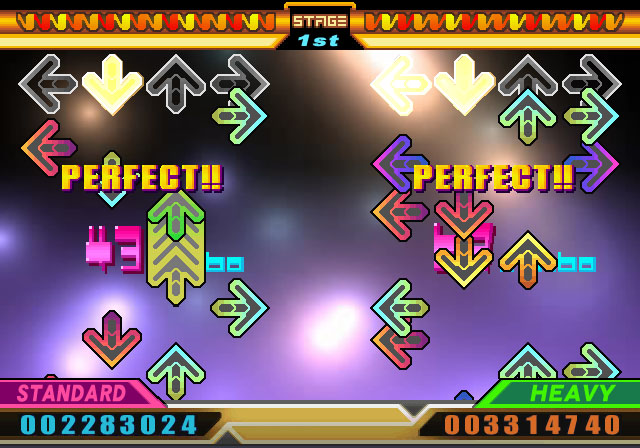
\includegraphics[width=0.43\textwidth]{Figures/dancedancerevolution}
  \end{center}
  \caption{Screenshot from Dance Dance Revolution, an example of a rhythm music game \cite{DDR}.}
\end{wrapfigure}

A music video game can be defined as a type of game that uses music or rhythm as an integral part of gameplay. This may involve pressing buttons in time with a song, whether on a conventional controller, and instrument controller or some kind of dance mat, singing into a microphone or creating original music. Players can often perform different parts of the same song together in local multiplayer games or over the Internet, providing enjoyable social experiences \cite{mvgdef}.

Some games exhibit a sandbox style that encourages a free-form gameplay approach whereas other a hybrid style, which combines musical elements with more traditional genres, for example puzzle games or shooters. 

Below we will briefly go over different types of music video games that can be found on the market.




\subsection{Music Memory Games}

The goal of the music memory game is to score player on their musical memory. Music track is presented to the user who then has to provide an appropriate response to each prompt from the game. Games may be based on different primary musical aspect (whether it is the rhythm, pitch or volume). However, a vast majority of the releases available on the market are rhythm-based.

\begin{figure}
        \centering
        \begin{subfigure}[b]{0.48\textwidth}
                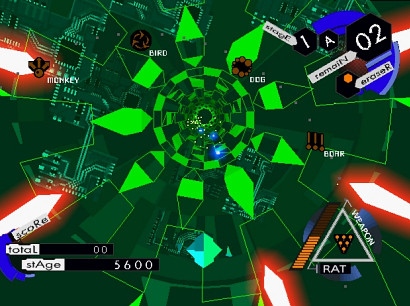
\includegraphics[width=\textwidth]{Figures/is}
                \caption{is - Internal Section - an example of a generative hybrid music game \cite{is}.}
                \label{fig:is }
        \end{subfigure}%
        ~ %add desired spacing between images, e. g. ~, \quad, \qquad, \hfill etc.
          %(or a blank line to force the subfigure onto a new line)
        \begin{subfigure}[b]{0.48\textwidth}
                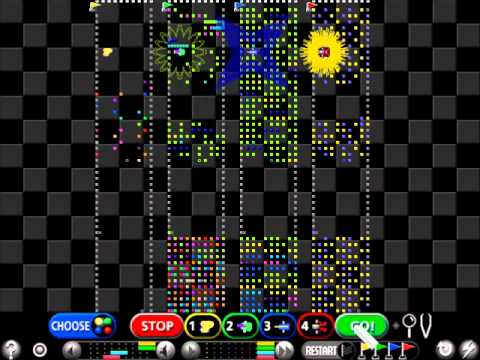
\includegraphics[width=\textwidth]{Figures/simtunes}
                \caption{SimTunes - an example of a free form music game \cite{simtunes}.}
                \label{fig:simtunes}
        \end{subfigure}
          \caption{Examples of music video games.}
        ~ %add desired spacing between images, e. g. ~, \quad, \qquad, \hfill etc.
\end{figure}


Rhythm games typically focus on dance or the simulated performance of musical instruments, and require players to press buttons in a sequence dictated on the screen. Doing so causes the game's protagonist or avatar to dance or to play their instrument correctly, which increases the player's score \cite{rhythmgame}. An example of such games could be Guitar Hero or Dance Dance Revolution.


\subsection{Free Form Music Games}

In free form music games, the main task of the user is to create content. This form of music game is often compared to non-game music synthesisers. Free form music games are somewhere between generative hybrid music games and non-game utilities, depending on the degree to which their gameplay relies on a driving underlying plot-line. An example of such game could be SimTunes, where the user is painting a picture using large pixels and each color represents a musical note. 


\subsection{Hybrid Music Games}

Hybrid music games are characterised by substantial and meaningful interactions between a player and the music game in a game that apparently belongs to a non-musical genre. This type of games can be further split into two sub-types.


Generative music video games make use of user’s actions. By monitoring interaction with the surroundings in the game, the mechanism generates sounds that are then integrated into the soundtrack, permitting the player’s direct interaction with the score. This encourages the creation of a synesthetic experience — when upon stimulation of one sense others activate, causing an involuntary experience. An example of such game could be Rez, which is a simple rail shooter. However, thanks to integrating sounds generated by player completing the normal task of rail-shooting, the score is dynamic.

Reactive music games, in contrast to generative one, employ music to determine the gameplay. In such games, the player takes cues from soundtrack to devise his gameplay. For example, iS - internal section, uses the music to determine the dynamic of the non-musical components of the game.

\begin{figure}
        \centering
        \begin{subfigure}[b]{0.48\textwidth}
                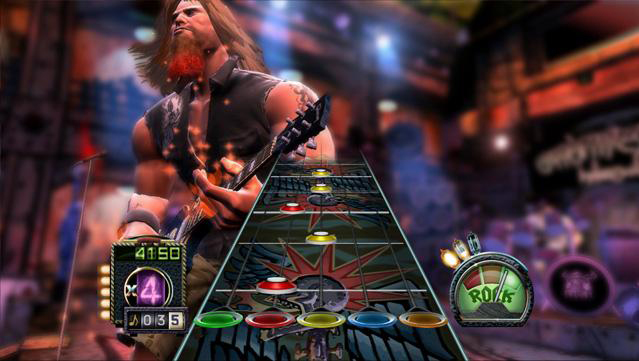
\includegraphics[width=\textwidth]{Figures/guitarhero}
                \caption{Screenshot from Guitar Hero - player is attempting to play a song \cite{ghscreen}.}
                \label{fig:Guitar Hero screenshot}
        \end{subfigure}%
        ~ %add desired spacing between images, e. g. ~, \quad, \qquad, \hfill etc.
          %(or a blank line to force the subfigure onto a new line)
        \begin{subfigure}[b]{0.48\textwidth}
                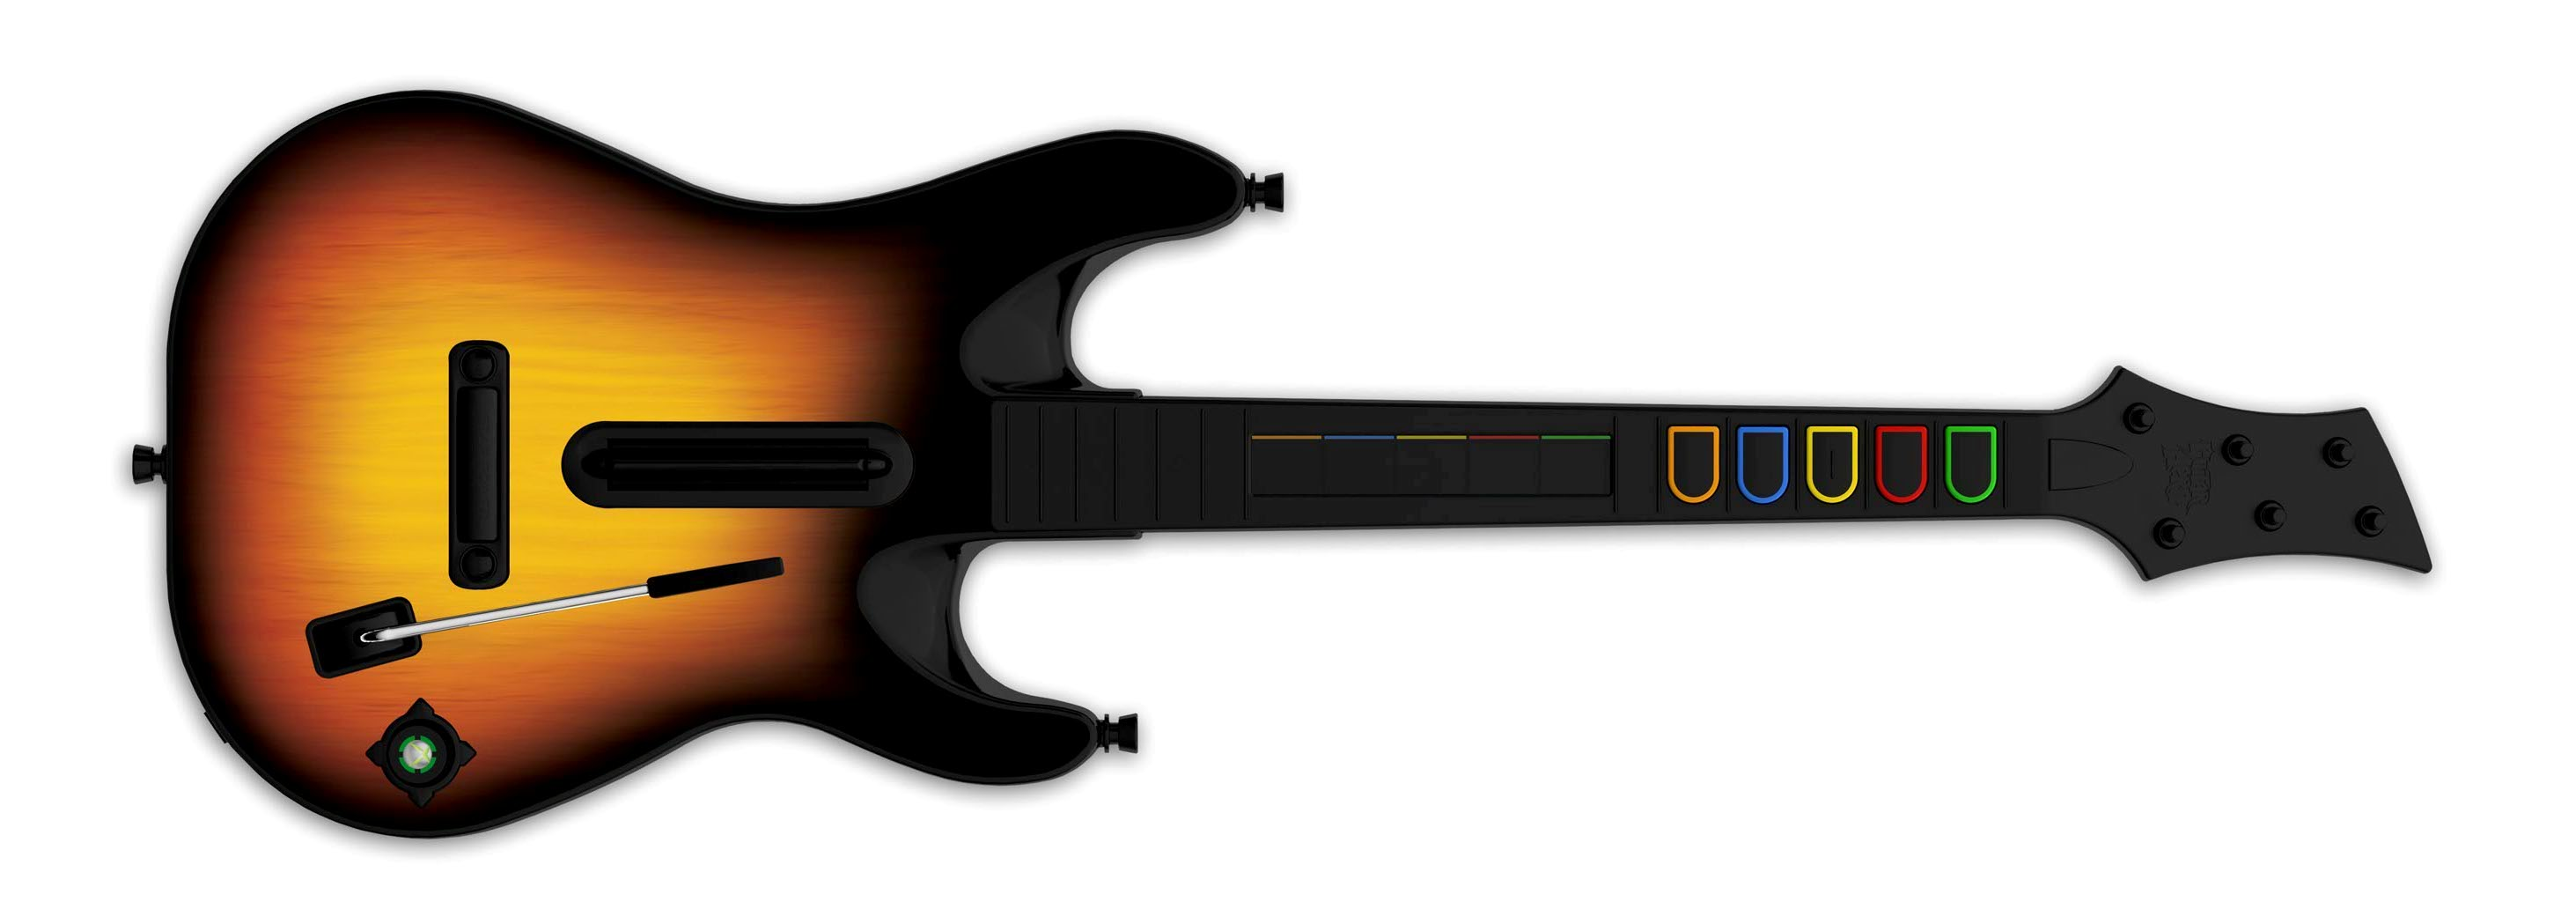
\includegraphics[width=\textwidth]{Figures/controller}
                \caption{A guitar shaped controller used in the game \cite{controller}.}
                \label{fig:Controller}
        \end{subfigure}
          \caption{Guitar Hero components}
        ~ %add desired spacing between images, e. g. ~, \quad, \qquad, \hfill etc.
\end{figure}


\section{Case Study - Guitar Hero}

Guitar Hero is one of the most popular franchises in the history of music games. The first of the series was published in 2005 by RedOctane and Harmonix. In the games, players instrument-shaped game controllers to simulate playing the instruments across numerous rock music songs. It is widely considered a highly entertaining game fully embracing the rhythm-based music game.


\subsection{The Controller}


Rather than a typical gamepad, Guitar Hero uses an instrument-shaped controller (guitar in the earlier releases, bass, microphone and drums in more recent ones). Playing the game with the guitar controller simulates playing an actual guitar, except it uses five coloured "fret buttons" and a "strum bar" instead of frets and strings, and an analogous mapping for the other instruments. They incorporate most of the real life techniques and motions that an instrumentalist would perform on a real instrument.


\subsection{The Gameplay}

The actual game itself works exactly as many other music titles do. At the bottom of the screen, a number of (varying depending of level of difficulty) buttons is shown. In each attempt, a series of notes moves across the screen and when a note aligns with a button, player is supposed to press a corresponding button, gaining points depending on the accuracy. If the player failed to achieve a certain amount of notes — his performance meter stays low for a longer time, he loses the game.

However, there are a couple minor improvements that Harmonix has made to the general music game formula. By acing certain notes in a song, a player is able to build up Star Power, which when unleashed, doubles up current point multiplier. Star Power also adds a bit of a strategic element - player not only earns more points when it is activated, but he can also raise your performance meter faster, enabling him to last longer when encountering a trickier part of a song.


\subsection{The Critique}

Without a doubt, Guitar Hero features a great selection of music. However, there will always be tracks missing, regardless of how many versions of Guitar Hero are released. People have different tastes and limiting a game to a set of tracks that everybody is supposed to enjoy is a really hard task. 

Some more advanced users familiar with Computer Science attempted to transcribe songs and to create new levels. However, this process is really difficult, especially for non computer scientists, discouraging an average user from fully making use of game’s capabilities. The producers, seeing the tendency, started releasing the in-app purchases to enable the players to extend their library and thus, keep the users. 

Implementing a feature of uploading some music preferred by the player would definitely improve user satisfaction. However, this might have not been achieved yet as the task itself is quite complex. Moreover, enabling the users to load in some music would deprive the company of their income sources.

\vspace{30pt}

\section{Introduction to Melody Extraction}

For a long time people were researching ways of estimating the fundamental frequency, be it with monophonic music recording or multi-pitch estimation. Melody extraction differs from both of those problems — unlike monophonic pitch estimation it handles polyphonic tracks and in contrast to multi-pitch estimation, it must also include a mechanism for source identification, to spot the voice carrying the melody within the polyphony.
To be able to evaluate the performance of the new algorithms, annual Music Information Retrieval Evaluation eXchange (MIREX) has been running since 2005. In this campaign, different models are evaluated against the same sets of music collections in order to obtain a quantitative comparison between methods and assess the accuracy of the current state-of-the-art in melody extraction \cite{comparison}.


\subsection{Melody}

The concept of “melody” ultimately relies on the judgment of people listening. This is why it will vary depending on the application context - whether we want to determine symbolic melodic similarity or transcribe a music track. 

In order to have a clear framework to work within, the Music Information Retrieval (MIR) community has adopted in recent years the definition proposed by \cite{melodydef}, “...the melody is the single (monophonic) pitch sequence that a listener might reproduce if asked to whistle or hum a piece of polyphonic music, and that a listener would recognise as being the 'essence' of that music when heard in comparison".

In practice, research has focused on "single source predominant fundamental frequency estimation" — which means a search for a main melody coming from a single sound source throughout the song analysed. As we can see, the subjective element is still present in this description of a melody as there might not be a definite way of deciding what predominant is. However, it fits well with our project’s objective — generating a game level based on changes in the pitch.


\subsection{Polyphonic Music}

Polyphony is a word derived from Greek poluph\={o}nosis meaning more than one sound — a texture consisting of two or more simultaneous lines of independent melody. This can be contrasted with homophony, where musical parts move generally in the same rhythm and one dominant melodic voice is accompanied by chords or monophony, where only one voice is found. 

However, in our case, the term polyphonic will simply refer to any type of music in which two or more notes can be played simultaneously. This can be achieved either by playing in different instruments (for example, voice, guitar and bass) or a single instrument capable of playing more than one more at a time (like a piano).


\subsection{Pitch, Tones, Fundamental Frequency}

Pitch is the most natural way of ordering sounds on a frequency-related scale. If sounds whose frequency is clear and stable enough to be distinguished from noise, they can be compared among  one another as “lower” or “higher”. Pitch is not an objective physical property — it depends on anatomy and physiology of the auditory system, which is a subject of an extensive study called psychoacoustics. 

A semitone is the smallest musical interval commonly used in Western tonal music. Two semitones constitute a tone.

The fundamental frequency $f_{\text{0}}$ is defined as the lowest frequency of a periodic waveform. A harmonic (or a harmonic partial) is any of a set of partials that are whole number multiples of a common fundamental frequency. This set includes $f_{0}$, which is a whole number multiple of itself (1 times itself).

Fundamental frequency can be thought of as the physical property most closely related to perception of pitch. This is why in this context pitch and fundamental frequency can be used interchangeably.


\subsection{Filter}

Any medium through which the music signal passes, whatever its form, can be regarded as a filter. However, we do not usually think of something as a filter unless it can modify the sound in some way. 

A digital filter is a filter that operates on digital signals, such as sound represented inside a computer. It is a computation which takes one sequence of numbers (the input signal) and produces a new sequence of numbers (the filtered output signal) \cite{filters}.


\subsection{Short Time Fourier Transform}

Short-time Fourier transform (STFT), is a signal processing method which is used in analysis of non-stationary signals with statistic characteristics varying with time.
In particular, STFT extracts several frames of the signal to be analysed with a window that moves with time. If we set the window size to be narrow enough, each frame extracted can be viewed as stationary so that Fourier transform can be used. With the window moving along the time axis, the relation between the variance of frequency and time can be identified \cite{STFT}.

The short time Fourier transform of a time-domain signal $y$ is denoted by the matrix $F \times N$, $F$ being the Fourier transform size and $N$ the number of analysis frames.

\section{Main Melody Extraction from Polyphonic Music}
In this section we will go over two different approaches to the problem of main melody extraction from polyphonic music, using source separation and a salience function. Then we will compare both methods to determine which one is more suitable for our project.

\vspace{50pt}

\subsection{Source Separation Based Approach}

\begin{wrapfigure}{r}{0.5\textwidth}
  \vspace{-50pt}

  \begin{center}
    \includegraphics[width=0.48\textwidth]{Figures/durrieudiagram}
  \end{center}
  \caption{Outline of system proposed by Durrieu: X is the STFT of the mixture signal, $p(\Xi|X)$ the posterior probability of a given melody sequence, and $\hat{\Xi} $ the desired smooth melody sequence\cite{durrieu}.}
\end{wrapfigure}


In polyphonic tracks the main melody can be represented by a specific source/filter model. In case of the leading vocal part, the vocal cords are treated as a source and the voice tract as a linear acoustic filter.

In their paper from 2011 \cite{durrieu}, authors presented an algorithm in which they assume that at any given time the signal observed is a mixture of two elementary signals - one corresponding to the main source and one to the background music. Therefore, the signal can be represented in an equation $x(t) = v(t) + m(t)$, where $v(t)$ stands for the source of the main melody and $m(t)$ is the background music. Interestingly, this equation also holds for the short time Fourier transform (STFT)  $X$, $V$ and $M$ respectively: $X = V + M$. The models proposed by Durrieu essentially aim at constraining the shapes of these STFT using temporal and spectral constraints. 


The likelihood of the vocal part V is calculated using two different frameworks. 

The first submission uses the source/filter Gaussian scaled mixture model (GSMM). In this model the source element refers to the excitation of the vocal folds and is therefore linked to the fundamental frequency of the sound $f_{\text{0}}$, while the filter part is characteristic of the vocal tract shape. This space of possibilities is then discretised so that we consider one possible filter frequency response, which is then used to calculate the likelihood of the vocal part knowing the filter and $f_{\text{0}}$.

Fig 2.4. A) shows the diagram of the GSMM model for the main voice part. Each source excitation $u$ is filtered by each filter $k$. The amplitudes for a frame $n$ and for all the couples $(k, u)$ are then applied to each of the output signals. At last a “state selector” sets the active state for the given frame.

The second model was derived from the first one to find a solution that would be more efficient to compute. The authors came up with a formulation that keep the source/filter model within an instantaneous mixture framework (IMM). In this model, for each source a set of filters is defined and at each frame, once every source is filtered and multiplied by a given amplitude, they are all added together.

The background music signal $m(t)$ can be thought of as a mixture of $R$ independent Gaussian sources $m_{r}(t)$. 
Each of the sources is centred and characterised by its power spectral density (PSD), which describes how the power of a signal or time series is distributed over the different frequencies. PSD can be estimated using a Covariance Method.
Due to the linearity of the Fourier transform, $M(f,t)$, the STFT of $m$, is also the instantaneous mixture of the $R$ spectra $M_{r}(f,t)$ of the sources: $M_{r}(f,t)$.
This together with STFT and an amplitude coefficient associated with each source is used to calculate the likelihood for each of the frequency bins. Let $M_{t}(f)$ be the STFT of the background signal at frame $t$ and frequency bin $f$, then we write its likelihood.

\begin{figure}
        \centering
        \begin{subfigure}[b]{0.47\textwidth}
                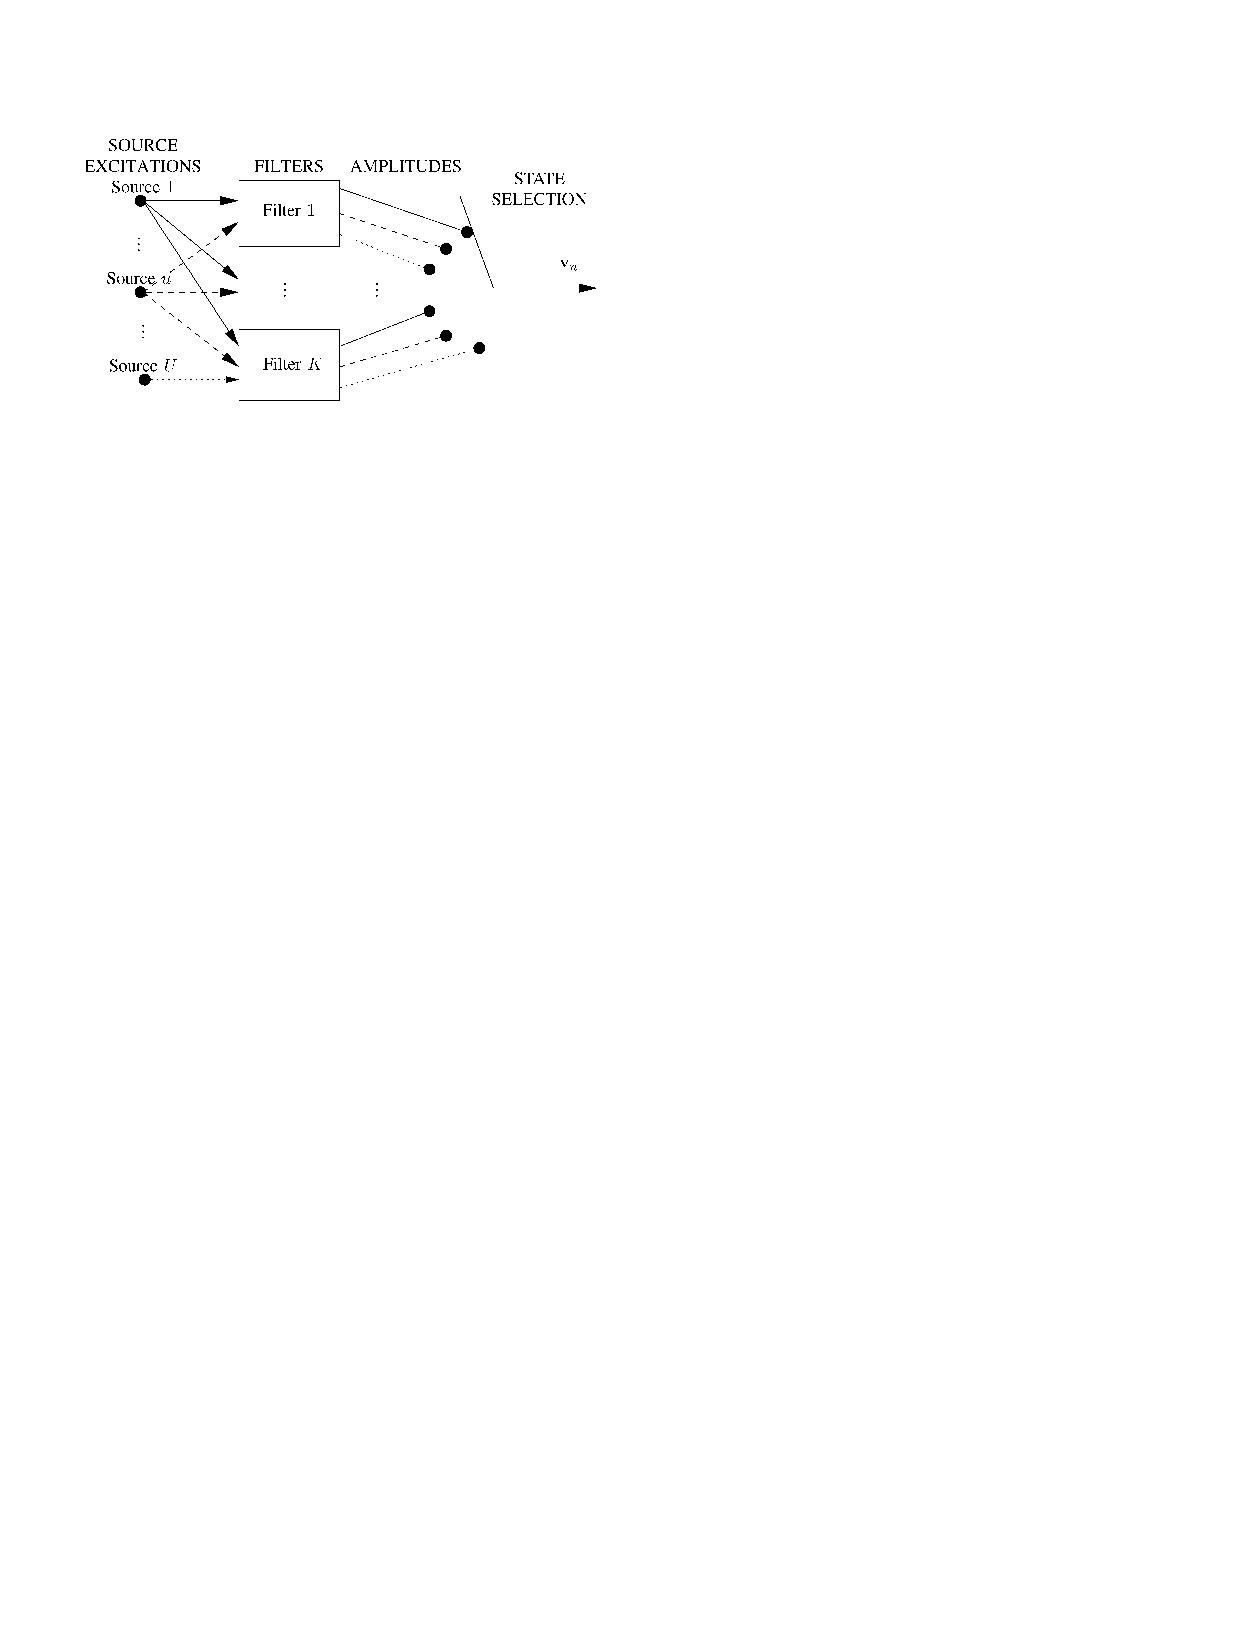
\includegraphics[width=\textwidth]{Figures/gsmm}
                \caption{Schematic principle of the generative GSMM. Each source u is filtered by each filter k. For frame n, the signal is then multiplied by a  given amplitude and a "state selector" then chooses the active state.}
                \label{fig:Guitar Hero screenshot}
        \end{subfigure}%
        ~ %add desired spacing between images, e. g. ~, \quad, \qquad, \hfill etc.
          %(or a blank line to force the subfigure onto a new line)
        \begin{subfigure}[b]{0.47\textwidth}
                \includegraphics[width=\textwidth]{Figures/imm}
                \caption{Schematic principle of the generative IMM. At each frame, all the U sources, each filtered by K filters, are multiplied by amplitudes and added together to produce the leading voice signal.}
                \label{fig:Controller}
        \end{subfigure}
          \caption{Diagram of both models presented in the paper\cite{durrieu}.}
        ~ %add desired spacing between images, e. g. ~, \quad, \qquad, \hfill etc.
\end{figure}

Once the parameters are estimated using the maximum likelihood criterion for each of the model, the Viterbi smoothing of the melody line is applied, obtaining a trade-off between the smoothness of the melody and its global energy in the signal. The Viterbi algorithm is a dynamic programming algorithm for finding the most likely sequence of hidden states – called the Viterbi path – that results in a sequence of observed events \cite{viterbi}.
 
The authors then parametrise the transitions between the possible main melody without disabling jumps from one note to the other. Using Wiener filtering - digital signal processing reducing the noise, using an statistical estimate of the signal using a desired data without such noise, a framework is implemented to separate the source. This way separated signals are obtained. Computing the energy for each frame of the separated main melody and thereafter thresholding allowed to discriminate between spurious notes and true positives.


\subsection{Salience Based Approaches}

\begin{wrapfigure}{r}{0.5\textwidth}
  \vspace{-60pt}

  \begin{center}
    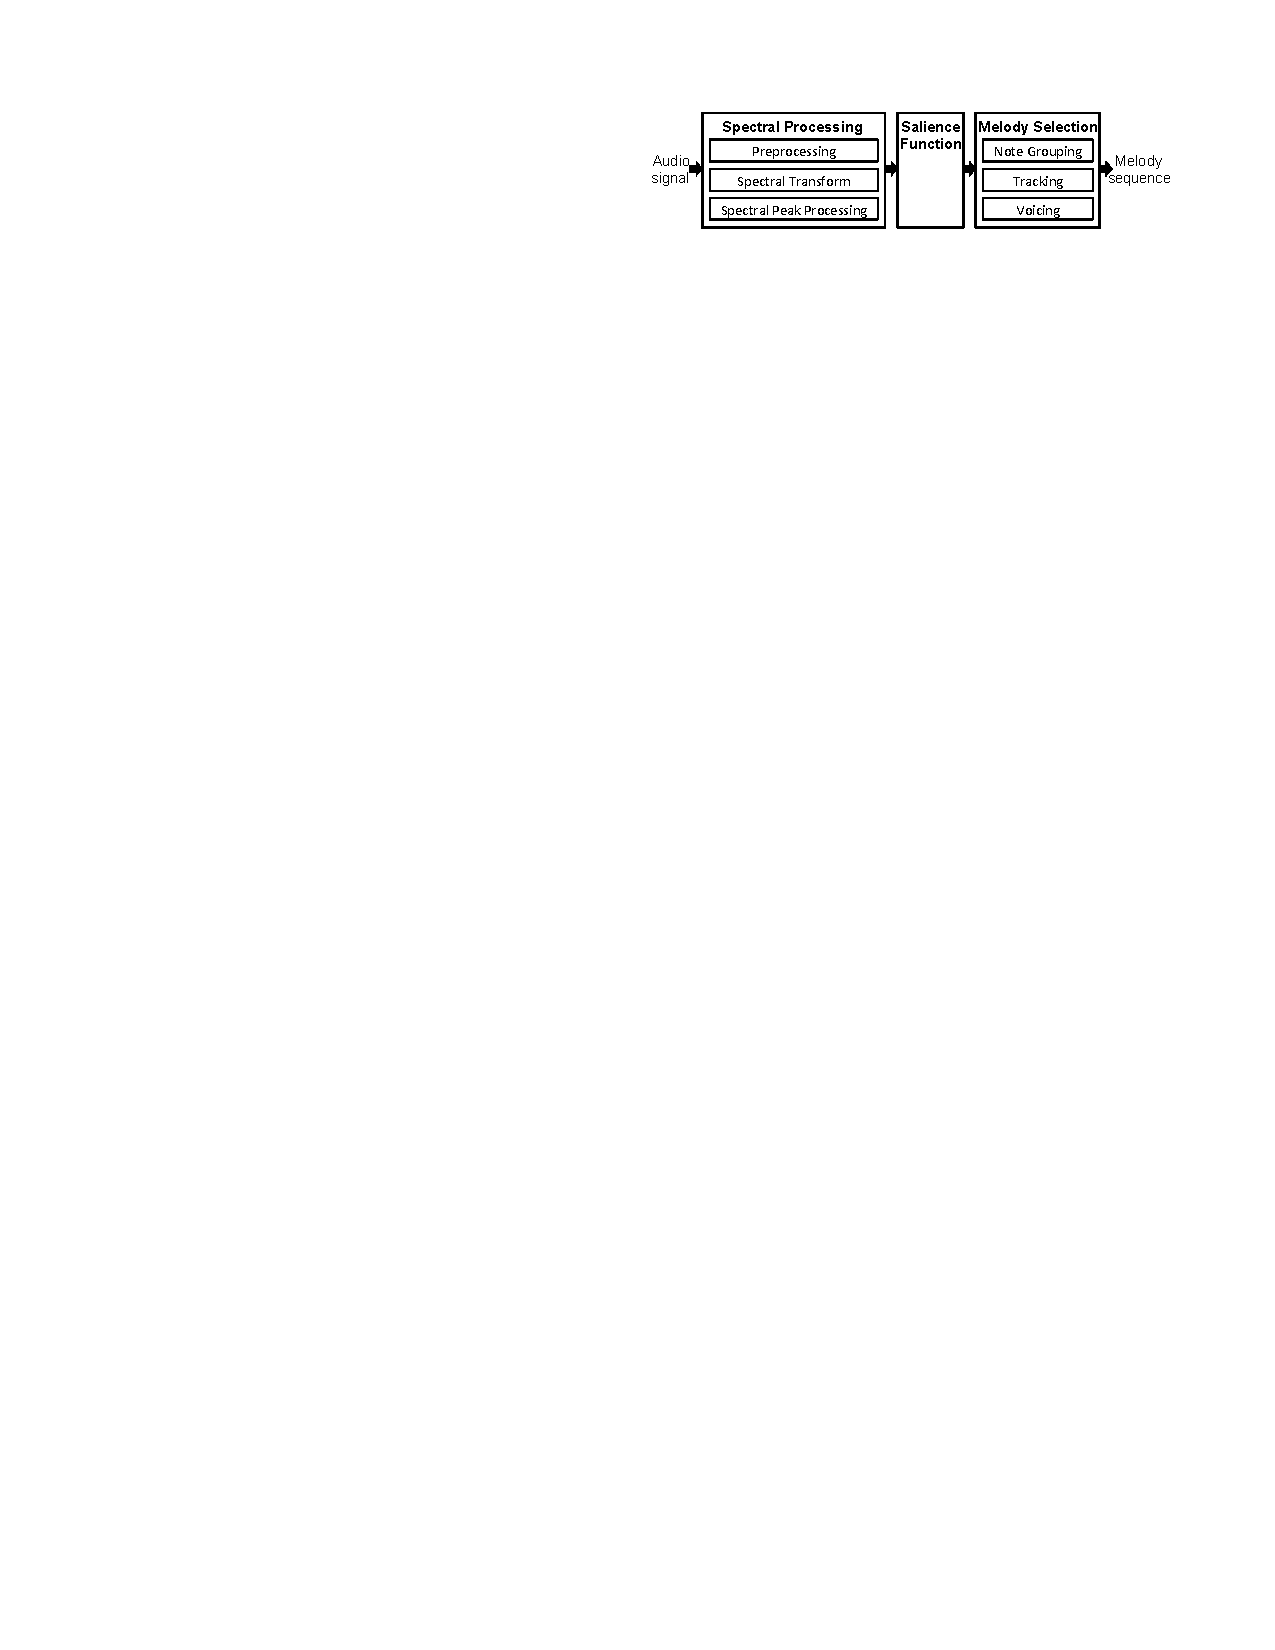
\includegraphics[width=0.48\textwidth]{Figures/salienceoveralldiagram}
  \end{center}
  \caption{Block diagram of four main blocks of the system by Salamon and G\'{o}mez: sinusoid extraction, salience function computation, pitch contour creation and melody selection \cite{comparison}.}
\end{wrapfigure}

This approach has been the most popular so far, with majority of algorithms evaluated at MIREX implementing it. It and can be split into several smaller stages, as seen in Figure 2.5. In particular, a method implemented in paper \cite{salamon} seems to be quite promising.

Usually as a first step, some sort of preprocessing is applied to the audio signal, usually to enhance the frequency content where we expect to find the melody. In particular, Salamon and G\'{o}mez apply an equal loudness filter, which enhances the frequencies to which the human ear is more perceptually sensitive, by taking a representative average of the equal loudness curves and filtering the signal by its inverse. 

This stage is followed by spectral transform — the signal is chopped into time frames and a transform function is applied to obtain a spectral representation of each frame.
This is achieved by applying the Short-Time Fourier Transform given by:

\begin{equation}
X_{l}(k) = \sum_{n=0}^{M-1} w(n) \times x(n + lH) e^{-j\frac{2 \pi}{N}kn}
\end{equation}

with a window length of 46.4ms. Here, $x(n)$ is the time signal, $w(n)$ the windowing function, $l$ the frame number, $M$ the window length, $N$ the FFT length and $H$ the hop size. Thanks to choosing a relatively small hop size, Salamon and G\'{o}mez achieve sufficient frequency resolution to identify different notes while maintaining adequate time resolution to track pitch changes in the melody over a short time. 

Having done this, we move to frequency/amplitude correction, where the spectral peaks are detected and used to construct a salience function. To avoid a relatively large error in the estimation of the peak frequency caused by binning them in the process of FFT, peak’s instantaneous frequency and amplitude are calculated. 

\begin{wrapfigure}{l}{0.5\textwidth}
  \vspace{-30pt}

  \begin{center}
    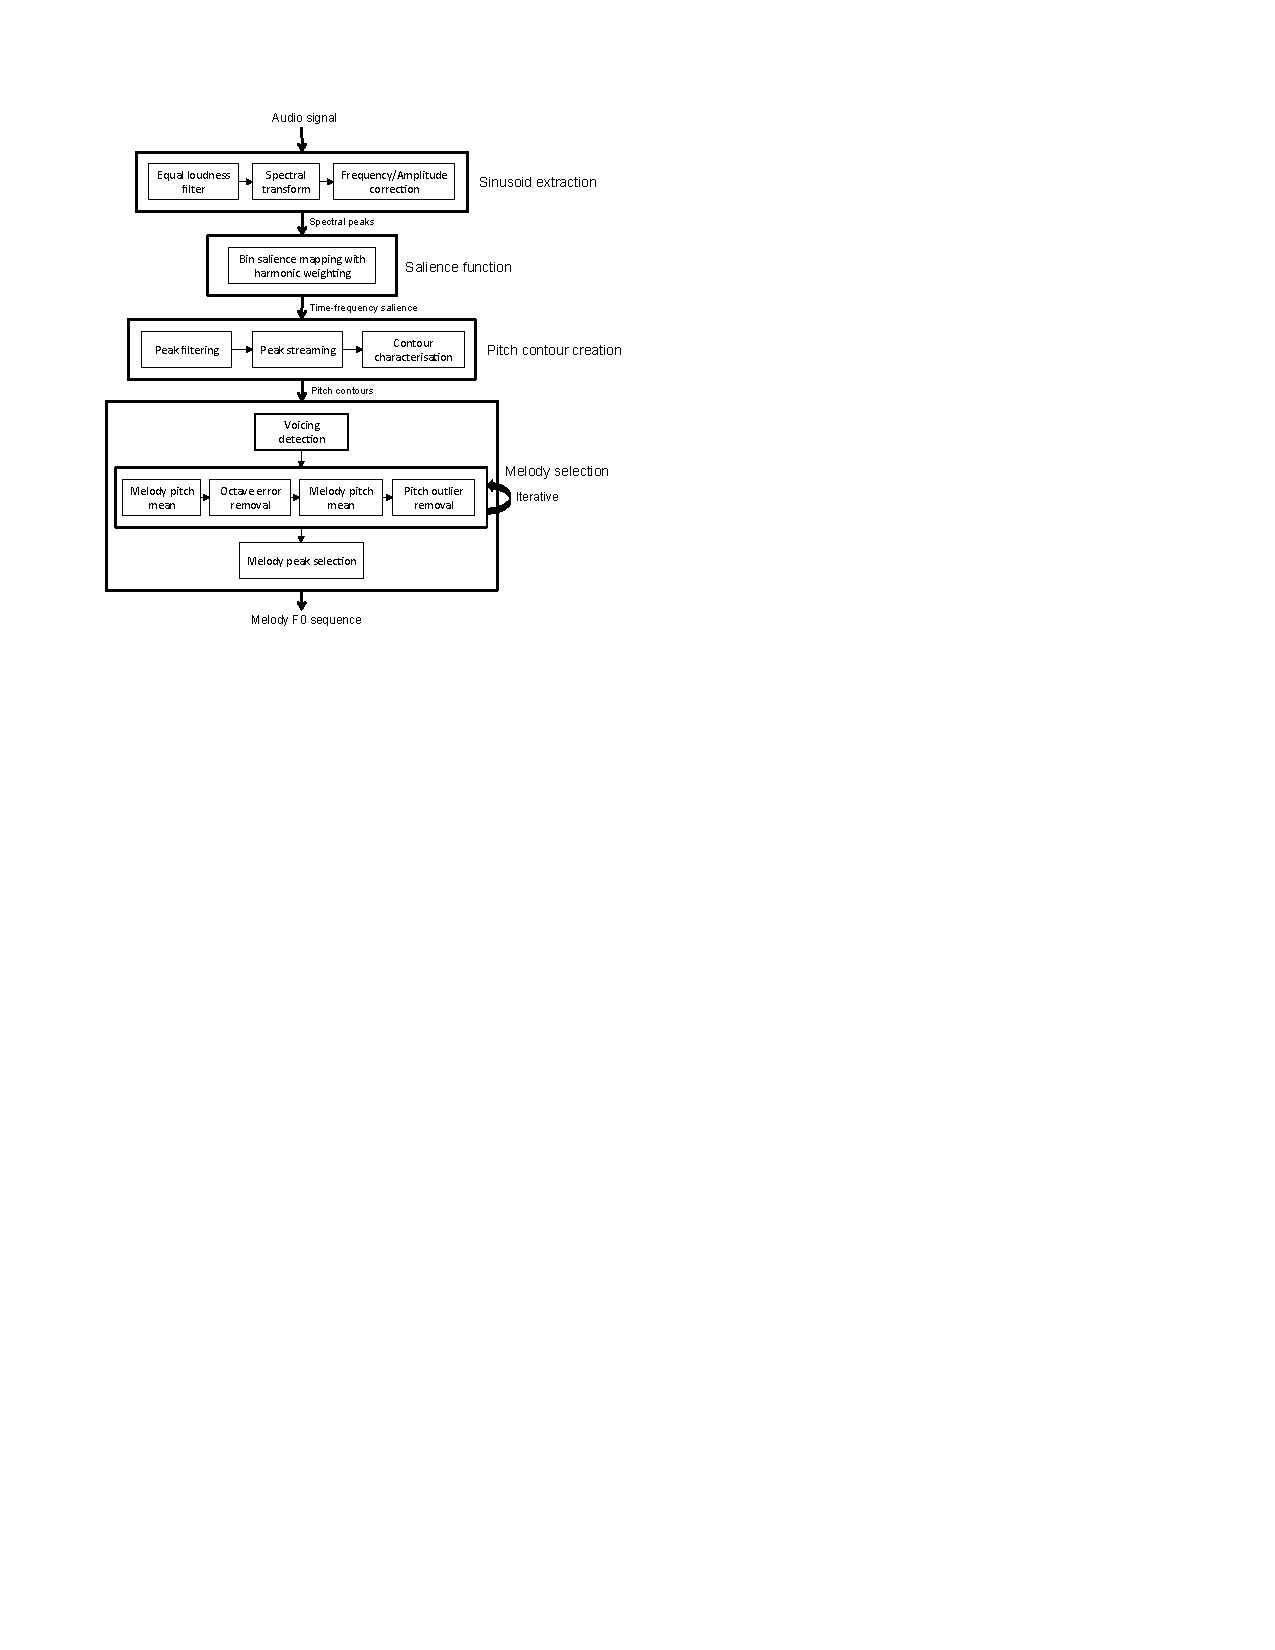
\includegraphics[width=0.48\textwidth]{Figures/salamon4blocksdiagram}
  \end{center}
  \caption{Block diagram of four main blocks of the system by Salamon and G\'{o}mez: sinusoid extraction, salience function computation, pitch contour creation and melody selection \cite{salamon}.}
\end{wrapfigure}

As we can see in figure 2.6, those three steps constitute the spectral processing. But at the core of the salience based algorithms lies the multi-pitch representation, i.e. the salience function — a representation of pitch salience over time. The peaks of this function form the $f_{0}$ candidates for the main melody. In the algorithm described by Salamon and G\'{o}mez, this computation is based on harmonic summation, where the salience of  a given frequency is computed as a sum of the weighted energies found at harmonics (integer multiples) of that frequency. Using only the peaks for the summation allows the authors to discard less reliable values and apply further frequency corrections. 

The salience function presented in the paper covers a pitch range of nearly five octaves from 55Hz to 1.76kHz.

Peaks of the salience function at each frame are now potential $f_{0}$ of the main melody. At this point some methods for melody extraction attempt to track the melody. However, Salamon and G\'{o}mez filter out the non-salient peaks, first by comparing them to the highest peak in the frame and then to a value computed using salience mean and standard deviation of all remaining peaks (in all frames). Now the peaks are grouped into pitch contours - time and pitch continuous sequences of salience peaks as shown in Figure 2.7.


\begin{figure}[h!]
  \centering
    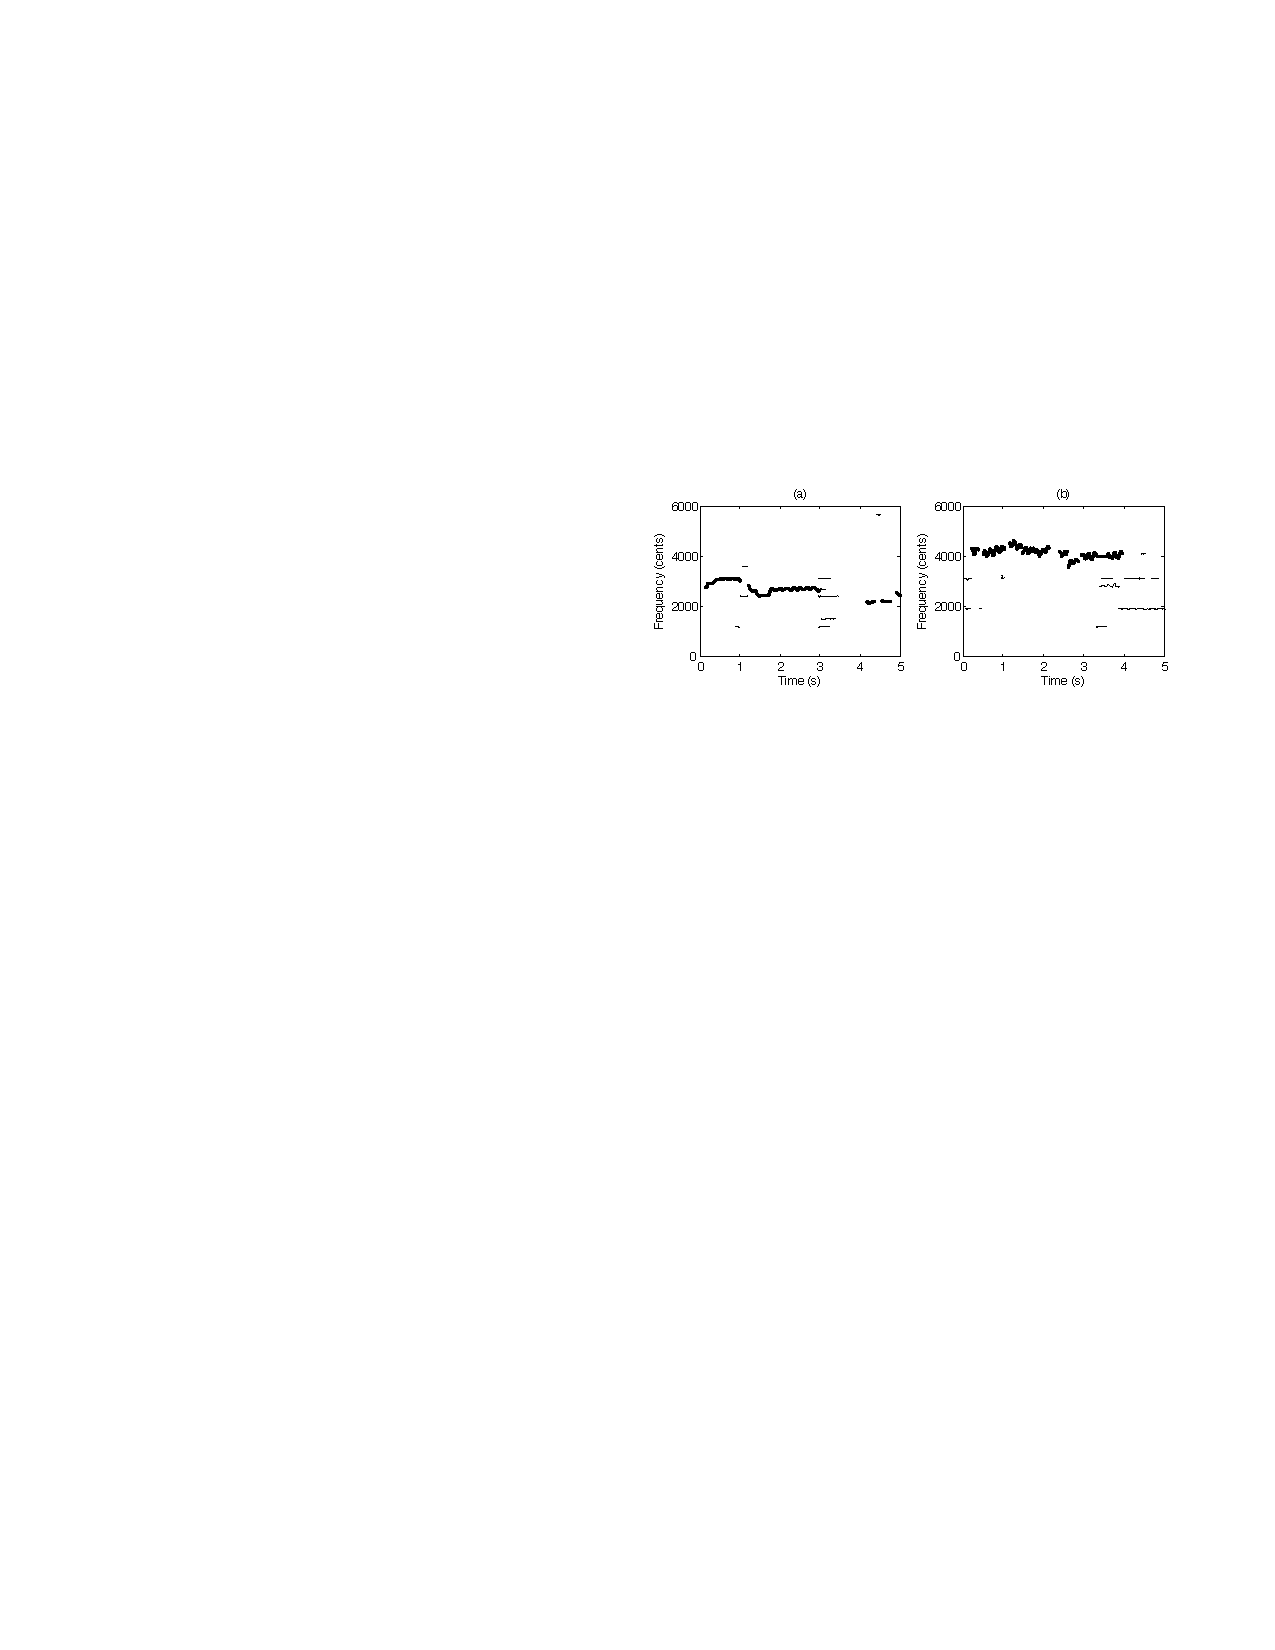
\includegraphics[width=0.7\textwidth]{Figures/pitchcontour}
      \caption{Pitch contours generated from excerpts of (a) vocal jazz and (b) opera. Melody contours are highlighted in bold\cite{salamon}.}

\end{figure}

Having created the pitch contours, Salamon and G\'{o}mez are faced with the task of determining which one belongs to the main melody. The authors define features based on contour pitch, length and salience.

Given the peaks of the salience function, we now have to determine which pitch values belong to the melody. This process is initiated by grouping peaks into continuous pitch contours, out of which a melody is selected later. 

The next main block in this algorithm shown in Figure 2.6 is the melody selection which is comprised of three steps: voicing detection, octave error minimisation/pitch outlier removal, and final melody selection.
As the name suggests, the aim of the voicing detection is to determine when the melody is present.


To filter out these contours Salamon and G\'{o}mez take advantage of the contour mean salience distribution.
By setting the threshold to a value slightly below the average contour mean salience of all contours in the excerpt $C_{s}$, we can filter out a considerable amount of non-melody contours. The authors define the following voicing threshold $\tau_{v}$ based on the distribution mean $C_{s}$ and its standard deviation $\sigma_{\overline{s}}$:
\begin{equation}
\tau_{v} = C_{s} - v \times \sigma_{\overline{s}}
\end{equation}

The parameter $v$ determines the lenience of the filtering - a high $v$ value might keep the false melody contours and a low value might filter out the melody contours.

It is also important to note that detecting certain characteristics in the contour increases a probability of it being the melody contour, for example in case of detecting a vibrato -  a regular, pulsating change of pitch, used to add expression to vocal and instrumental music. \cite{vibrato}

Next step in the melody selection described by Salamon and G\'{o}mez in their paper is octave errors and pitch outliers removal.  

In particular, the octave errors are the main sources of errors in melody extraction systems, when a multiple or sub-multiple of $f_{0}$ is reported as the main melody. 

To detect such errors, contour trajectories are compared by computing distance between their values on a per-frame for the region they overlap in and computing the mean over this region.
If the mean distance is within $1200\pm50$ cents, the contours are considered octave duplicates.

Secondly, Salamon and G\'{o}mez use the relationship between neighbouring contours (in time) to decide which of the duplicates is the correct one. Their approach is based on two assumptions: firstly, that most (though not all) of the time the correct contour will have greater salience than its duplicate (the salience function parameters were optimised to this end). Secondly, that melodies tend to have a continuous pitch trajectory avoiding large jumps, in accordance with voice leading principles.

The method iteratively computes the $\overline{P(t)}$ - pitch trajectory that represents the time evolution of the melody's pitch.
It then detects and removes an octave duplicate as well as  the "pitch outliers” – contours more than one octave above or below the pitch mean and then it is recalculated. Authors empirically discovered that 2 iterations of this process are enough to get a good approximation of the true trajectory of the melody, which is then passed to the final stage of the model - the final melody selection.

At this stage, there is often only one peak to be chosen as the main melody. When there is still more than one contour present in a frame, the melody is selected as the peak belonging to the contour with the highest total salience $C_{\sum s}$. If no contour is present the frame is regarded as unvoiced.

\subsection{Comparison of both approaches}

In their paper \cite{comparison}, authors attempted to compare multiple melody extraction algorithms created since 2005. One of the methods, used also by MIREX, is based on the per-frame comparison, considering different measures:


\begin{description}
\item[Voicing Recall Rate] - the proportion of frames labeled as melody frames in the ground truth that are estimated as melody frames by the algorithm.
\item[Voicing False Alarm Rate] - the proportion of the frames labeled as non-melody in the ground truth that are mistakenly estimated as melody frames by the algorithm.
\item[Raw Pitch Accuracy] - the proportion of melody frames in the ground truth for which $f_{\tau}$ is considered correct (i.e. within half a semitone of the ground truth). 
\item[Raw Chroma Accuracy] - as raw pitch accuracy, except that both the estimated and ground truth $f_{0}$ sequences are mapped onto a single octave. This gives a measure of pitch accuracy which ignores octave errors.
\item[Overall Accuracy] - this measure combines the performance of the pitch estimation and voicing detection tasks to give an overall performance score for the system. It is defined as the proportion of all frames correctly estimated by the algorithm, where for non-melody frames this means the algorithm labeled them as non-melody, as for melody frames the algorithm both labeled them as melody frames and provided a correct $f_{0}$ estimate for the melody (again, within half a semitone of the ground truth).
\end{description}


\begin{figure}[h!]
  \centering
    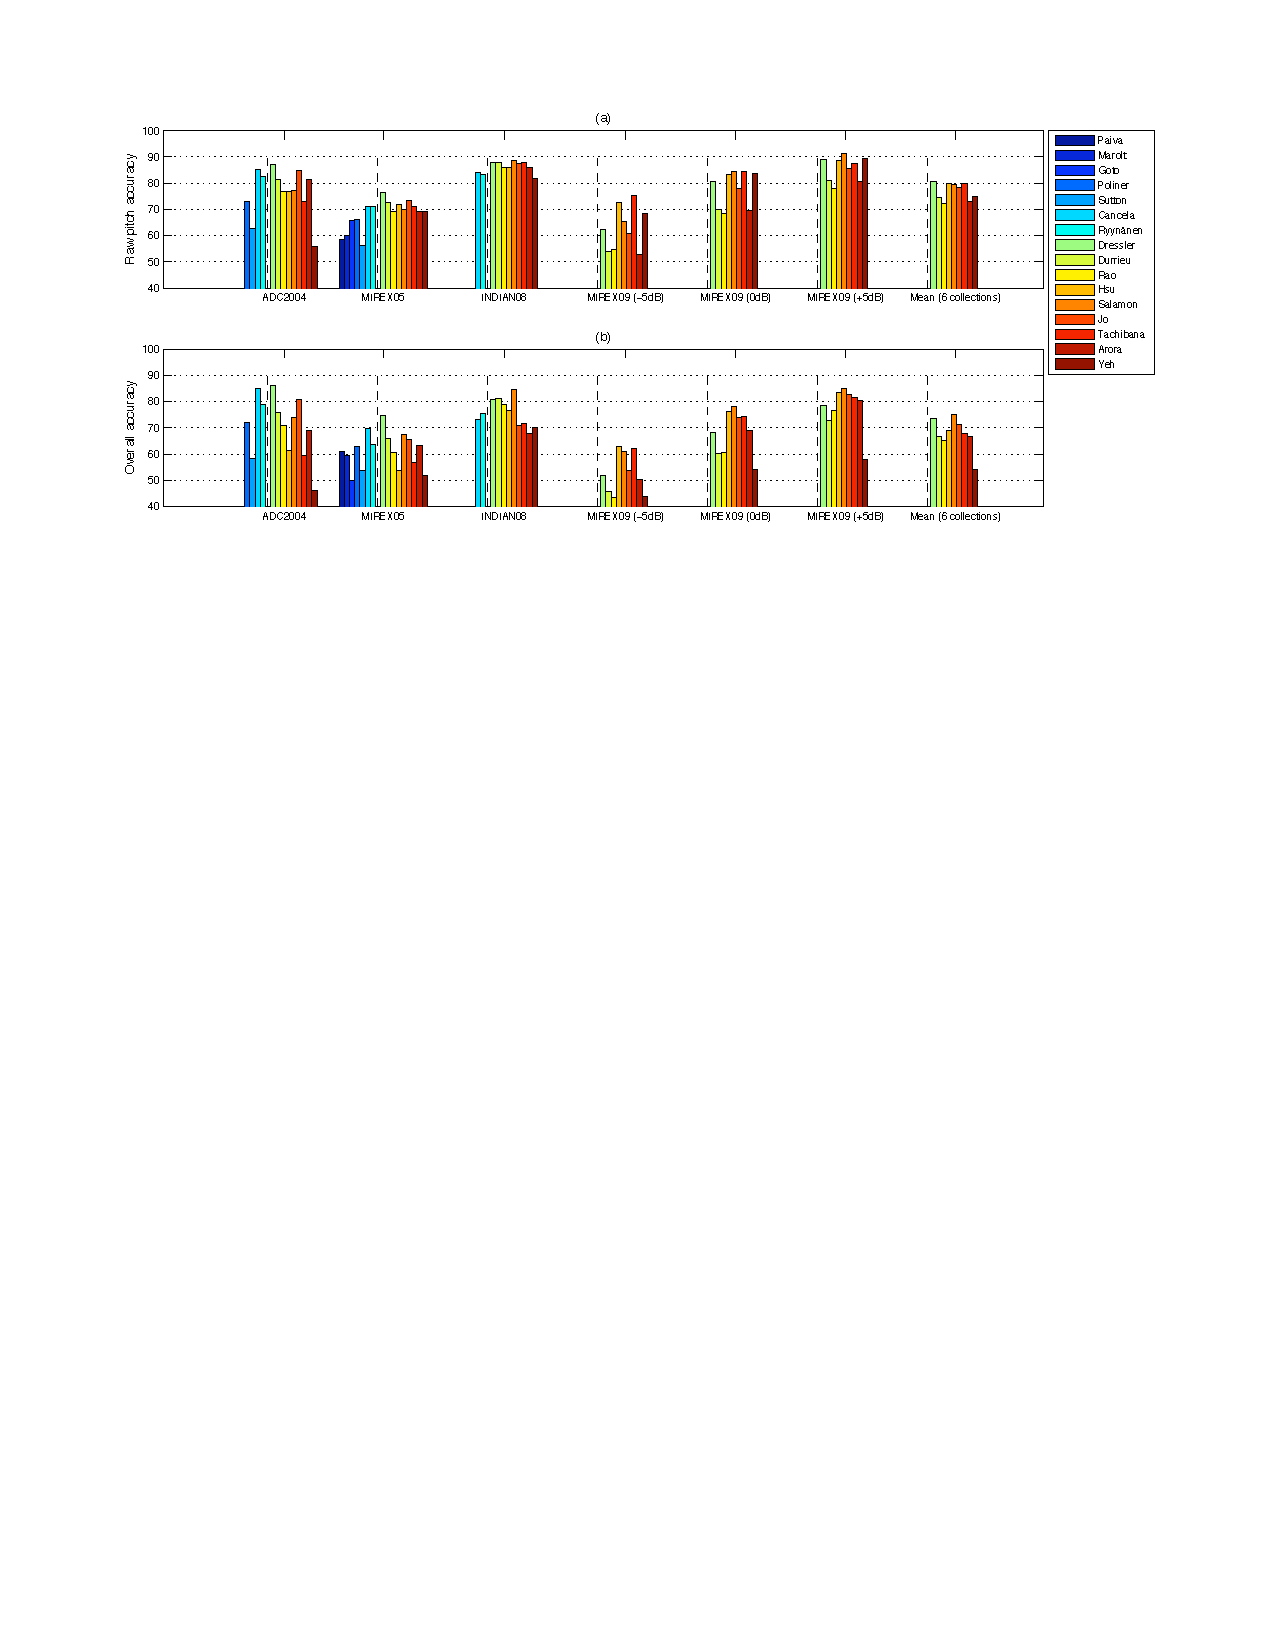
\includegraphics[width=\textwidth]{Figures/comparisonall}
      \caption{a) Raw pitch accuracy and b) overall accuracy obtained in MIREX by 16 melody extraction algorithms evaluated in \cite{comparison}. The vertical dashed line separates the algorithms that were only evaluated on some collections (left of the line) from those evaluated on all six collections (right of the line)\cite{comparison}.}
\end{figure}


In Figure 2.8. the authors presented results obtained by the algorithms evaluated at MIREX. To get a general idea of the performance of the algorithms, it is sufficient to focus on two evaluation measures.
The raw pitch accuracy, presented in Figure 2.8 a) represents how well the algorithm tracks the pitch of the melody. The overall accuracy on the other hand, as shown in Figure 2.8 b), combines this measure with the efficiency of the algorithm's voicing detection, meaning the voicing-related measures are also reflected in this measure.

As we can see, some collections are generally hard to analyse (for example MIREX09 -5db), in general the collections yield different results for different algorithms. This allows us to spot pros and cons of each approach investigated.

We can also notice that the raw pitch accuracy gradually improved from 2005 to 2009, after which it stayed relatively unchanged. Overall we can see that the average pitch accuracy over a collection lies between 70-80%.

On the other hand, when it comes to overall accuracy, the performance goes down compared to the raw pitch accuracy for all algorithms due to voicing detection being factored into the results. The importance of this step depends on the intended use of the algorithm. Generally, the overall accuracy results lie between 65-70%.

Finally, an important factor in assessment of an algorithm is its complexity. While deriving O-notation is too complex for some of the algorithms, generally it is observed that algorithms involving source separation are significantly more computationally complex than salience based approaches Unfortunately, there is no specific data provided by Salamon and G\'{o}mez [9] or by Durrieu [5] on their algorithms.

In conclusion, we believe the solution proposed by Salamon and G\'{o}mez is better fitted to the purpose of this project. The paper presents it in a much clearer way and, what is most important, it outperforms the one created by Durrieu significantly, as seen in Figure 2.8.. In addition to this, according to tendency it is less computationally expensive, which is quite important when it comes to game designing as we do not want to keep the user waiting for a long time for his level to generate and load.

\section{Mood Detection}
It is well known that music can convey emotion and modulate mood. That is why the relation between musical sounds and their influence on the listener’s emotion has been well studied.

One of the first publications on emotion detection in music is credited to Feng, Zhuang, and Pan \cite{moodold}. They employ Computational Media Aesthetics to detect mood for music information retrieval tasks. The two dimensions of tempo and articulation are extracted from the audio signal and are mapped to one of four emotional categories; happiness, sadness, anger, and fear. 
After that, feature called relative tempo is calculated, and after the mean and standard deviation of the feature called average silence ratio in the presented computational articulation model are calculated, a simple Back Propagation neural network classifier is trained to detect mood.

In publication by Yang, Lin, Su and Chen \cite{mood}, the authors presented a tool which recognises a mood in a musical track, allowing a user to then choose the song they want to play by deciding on emotions it is supposed to represent.
Specifically, the authors formulate music emotion recognition as a regression problem to predict the arousal and valence values (AV values) of each music sample directly.

Potentially, the second approach described seems more appropriate for our project as it allows for better granularity in the melody emotion detection and, hence, wider variety of changes in the game's environment. However, this area of the project is left to be further researched.


\section{Level Generation}
It is not really surprising that there is no current literature on the problem of automatically generating Guitar Hero buttons given an arbitrary piece of music.
However, we believe an algorithm can be developed where the buttons can be mapped to the $f_{0}$ in the main melody extracted by main melody extraction algorithm. 
% Chapter Template

\chapter{Design and Implementation} % Main chapter title

\label{Chapter5} % Change X to a consecutive number; for referencing this chapter elsewhere, use \ref{ChapterX}

\lhead{Chapter 5. \emph{Design \& Implementation}} % Change X to a consecutive number; this is for the header on each page - perhaps a shortened title


In this chapter we will go over the implementation process of the project. We will describe various choices we made, justifying them in the context of our objectives. 

First we will describe our solution to the mood detection problem. We first try to determine which musical features are the most correlated to the AV values of the music's emotion. Then, by training a neural network with data containing chosen features we will create a way of determining the arousal and valence value of any musical track, which will be later used in the implementation of our game. In addition to this, by investigating the impact of different parameters we will make sure out network has as good performance and accuracy as possible.

Next, we will move on to main melody detection by looking at two algorithms - one using source separation based approach and the other using the salience based approach. We will evaluate performance of both of them on data from recent pop culture to determine their performance and fitness in this project.

The next section will describe our attempt to automated music segmentation.

Last, but not least, we will talk about the game itself, its architecture, flow of use and design choices made.

\vspace{20pt}

\section{Mood Detection}

A common reason for engaging in music listening is that music is an effective means of conveying and evoking emotions. Although they may be subjective, based in part on the listener’s cultural and musical background or preferences, there are commonalities in perceived emotion across different listeners based on the characteristics of the music. Several studies have attempted to predict emotion conveyed during music listening. In our approach, we decided to represent the emotion connected to the music using a two-dimensional space with valence on the x-axis and arousal on the y-axis, first proposed by R. E. Thayer \cite{Thayer}.

As we described in Section \ref{sec:emotionClass}, there is a relation between valence and arousal values for a musical track and the moods perceived by people. In essence, the high arousal is connected to how energetic the music is, whereas valence refers to how positive (or negative) the emotions in the track are. 

\vspace{10pt}

\subsection{Choice of Features}
Using Essentia library \cite{essentia}, we implemented an extractor to retrieve certain features from a song, which we would expect to have certain impact on the perceived mood of a musical piece:

\begin{description}

\item[average loudness] - dynamic range descriptor. It rescales average loudness into the [0,1] interval on a per window basis. The value of 0 corresponds to signals with large dynamic range, 1 corresponds to signal with little dynamic range. This could indicate the level of the arousal, with higher loudness implying higher arousal value. We believe this relation could be quite intuitive - sad or peaceful songs tend to be quiet whereas excited or angry emotions are usually linked to louder tracks.

\item[means and derivatives of variance of rates of silent frames] in a signal for thresholds of 20, 30 and 60db. We believe that the values could influence the arousal levels, as the more and the bigger the silent gaps, the sadder / more peaceful the track seems to be, implying the low arousal value. When examining multiple musical tracks we have noticed that the happier or angrier songs can also have such silent gaps, but they tend to be much shorter.

\item[dynamic complexity] - computed on 2 second windows with 1 second overlap. The dynamic complexity is the average absolute deviation from the global loudness level estimate on the dB scale. It is related to the dynamic range and to the amount of fluctuation in loudness present in a recording. We believe this feature would have an impact on both examined values. However, similarly to the loudness level, arousal should be influenced more - as more dynamic songs (excited or angry) are more likely to suffer from loudness changes, whereas more phlegmatic ones (sad or peaceful) tend to keep the same dynamic complexity level.

\item[BPM] - beats per minute value according to detected beats. This feature should be correlated with the arousal level - intuitively, the faster the song, the more energetic it seems. 

\item[spectral centroid] - centroid statistics describing the spectral shape. It indicates where the ``center of mass'' of the spectrum is. Perceptually, it has a robust connection with the impression of ``brightness'' of a sound - an indication of the amount of high-frequency content in a sound. Timbre researchers consider brightness to be one of the perceptually strongest distinctions between sounds \cite{timber}, and formalise it acoustically as an indication of the amount of high-frequency content in a sound. That is why we believe the spectral centroid might be related to both valence and arousal.

\item[spectral RMS] (root mean square) - in physics it is a value characteristic of a continuously varying quantity, such as a cyclically alternating electric current or a sound. It is obtained by taking the mean of the squares of the instantaneous values during its duration or a cycle. This is linked to the loudness of the sound. This is why we believe that it might have an impact on arousal, but we do not exclude its impact on valence.

\item[spectral energy] - the energy E{s} of a continuous-time signal x(t) defined as: 
\begin{equation}
E{s}  =  \langle x(t), x(t)\rangle =  \int_{-\infty}^{\infty}{|x(t)|^2}dt
\end{equation}

Signal energy is always equal to the summation across all frequency components of the signal's spectral energy density. 
There have been some research focusing on relation between spectral energy and singing voice. In particular, in their paper \cite{spectralenergy}, S. Ferguson, D. T. Kenny and D. Cabrera were investigating the relation between the value and the experience of male singers. This makes for an interesting case worth considering in our research.

\item[mean and derivative of variance of beat loudness] -  spectral energy computed on beats segments of audio across the whole spectrum, and ratios of energy in 6 frequency bands. We suspect that the low value of the beat loudness could imply a low arousal.

\item[key and its scale] estimated key and its scale (major or minor) using Temperley’s profile. 
In music theory, the term key is used in many different and sometimes contradictory ways. A common use is to speak of music as being 'in' a specific key, such as ``in the key of C major or in the key of F\#''. Sometimes the terms 'major' or 'minor' are appended, as 'in the key of A minor' or 'in the key of B major'.
Broadly speaking the phrase 'in key of C' means that C is music's harmonic centre or tonic (the first degree of the scale, or the root of the scale). 
The terms 'major' and 'minor' further imply the use of a major scale or a minor scale. Thus the phrase 'in the key of E major' implies a piece of tonal music harmonically centred on the note E and making use of a major scale whose first note, or tonic, is E. 
We believe that those features can have an impact on both arousal and valence - songs performed in minor scale are traditionally connected to being sad, whereas the major scale is usually linked to positive emotions.

\item[scale and key of the chords] taken as the most frequent chord, and scale of the progression, whether major or minor. Scale commonly known to have a big influence on our perception on music \cite{keys}. It seems to be mostly the result of cultural conditioning as when people listen to tunes, they rely heavily on their memory. Such constant stimulus to our musical memory helps to generate expectations of what might come next in a tune or preserve the sound - emotion relation.

\item[means of zero-crossing rate] - the rate of sign-changes along a signal, i.e., the rate at which the signal changes from positive to negative or back. This feature has been used heavily in music information retrieval, being a key feature to classify percussive sounds. We believe it could be related to the arousal value. Music has a fairly normal distribution of frames with lower and higher zero-crossing rates. Speech however displays a much more skewed distribution. This could have an impact on songs where the vocals are quite rapid and energetic, for example rap music, and therefore might have a significant impact on mood recognition in our system.
ZCR is defined formally as: 
\begin{equation}
ZCR = \frac{1}{T-1} \sum_{t=1}^{T-1} {{\mathbb I}\left\{{s_t s_{t-1} < 0}\right\}}
\end{equation}

\item[pitch salience of a spectrum] - given by the ratio of the highest auto correlation value of the spectrum to the non-shifted auto correlation value.  Unpitched sounds (non-musical sound effects) and pure tones have an average pitch salience value close to 0 whereas sounds containing several harmonics in the spectrum tend to have a higher value. We think the value could have an effect on both the valence and arousal as pitch salience is often described as the probability of noticing a tone or clarity or strength of tone sensation.

\item[mean and derivative of variance of sensory dissonance] (to distinguish from musical or theoretical dissonance) of an audio signal given its spectral peaks. Sensory dissonance measures perceptual roughness of the sound and is based on the roughness of its spectral peaks. Given the spectral peaks, the algorithm estimates total dissonance by summing up the normalised dissonance values for each pair of peaks. These values are computed using dissonance curves, which define dissonance between two spectral peaks according to their frequency and amplitude relations. Dissonance could be related to low valence.

\end{description}

\begin{figure}
        \centering
        \begin{subfigure}[b]{0.48\textwidth}
                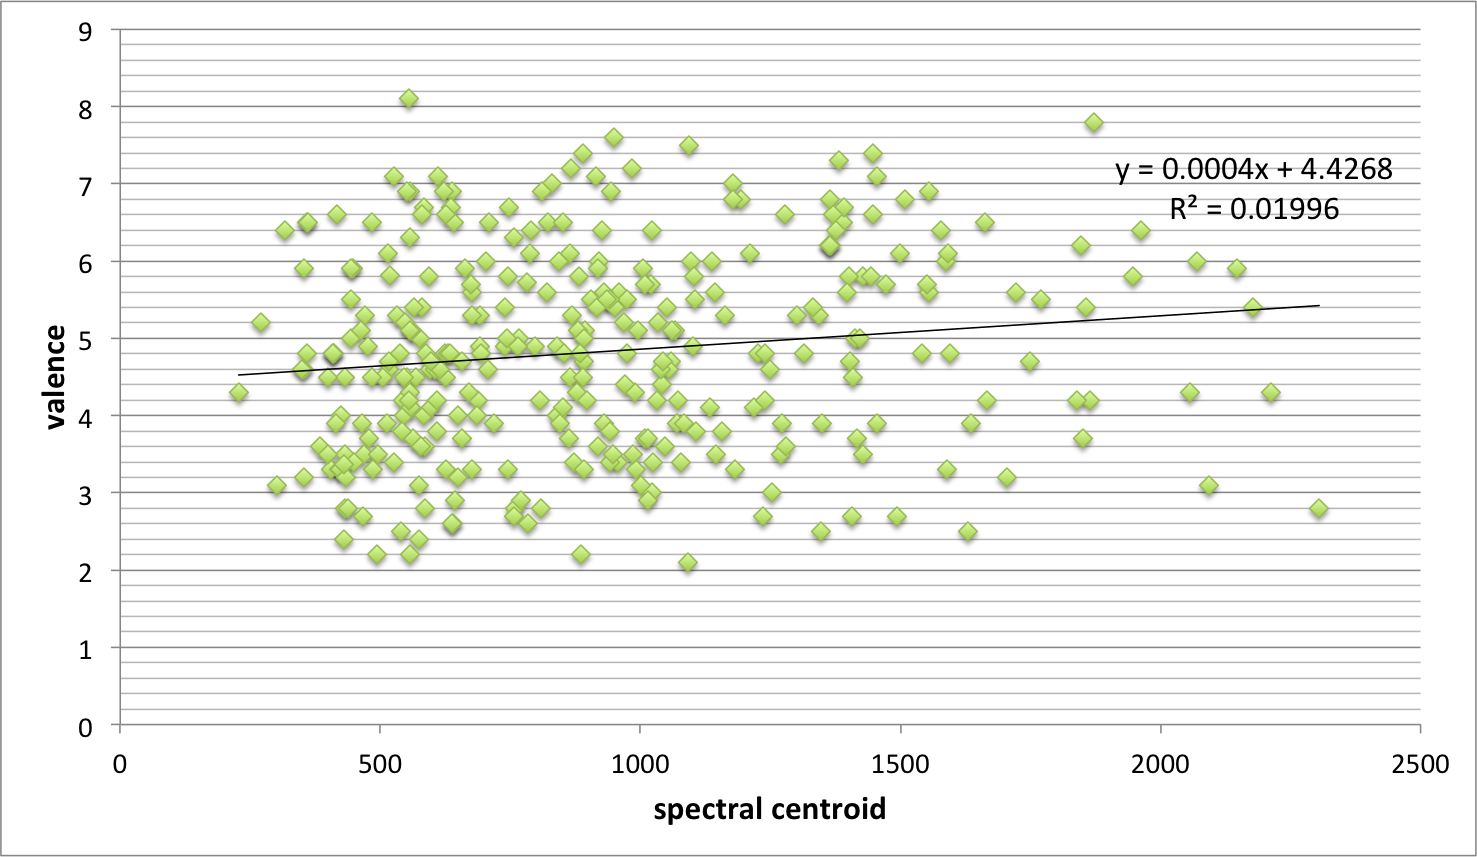
\includegraphics[width=\textwidth]{Figures/spectralcentroid-valence}
                \caption{A graph representing a correlation between spectral centroid and valence values.}
        \end{subfigure}%
        ~ %add desired spacing between images, e. g. ~, \quad, \qquad, \hfill etc.
          %(or a blank line to force the subfigure onto a new line)
        \begin{subfigure}[b]{0.48\textwidth}
                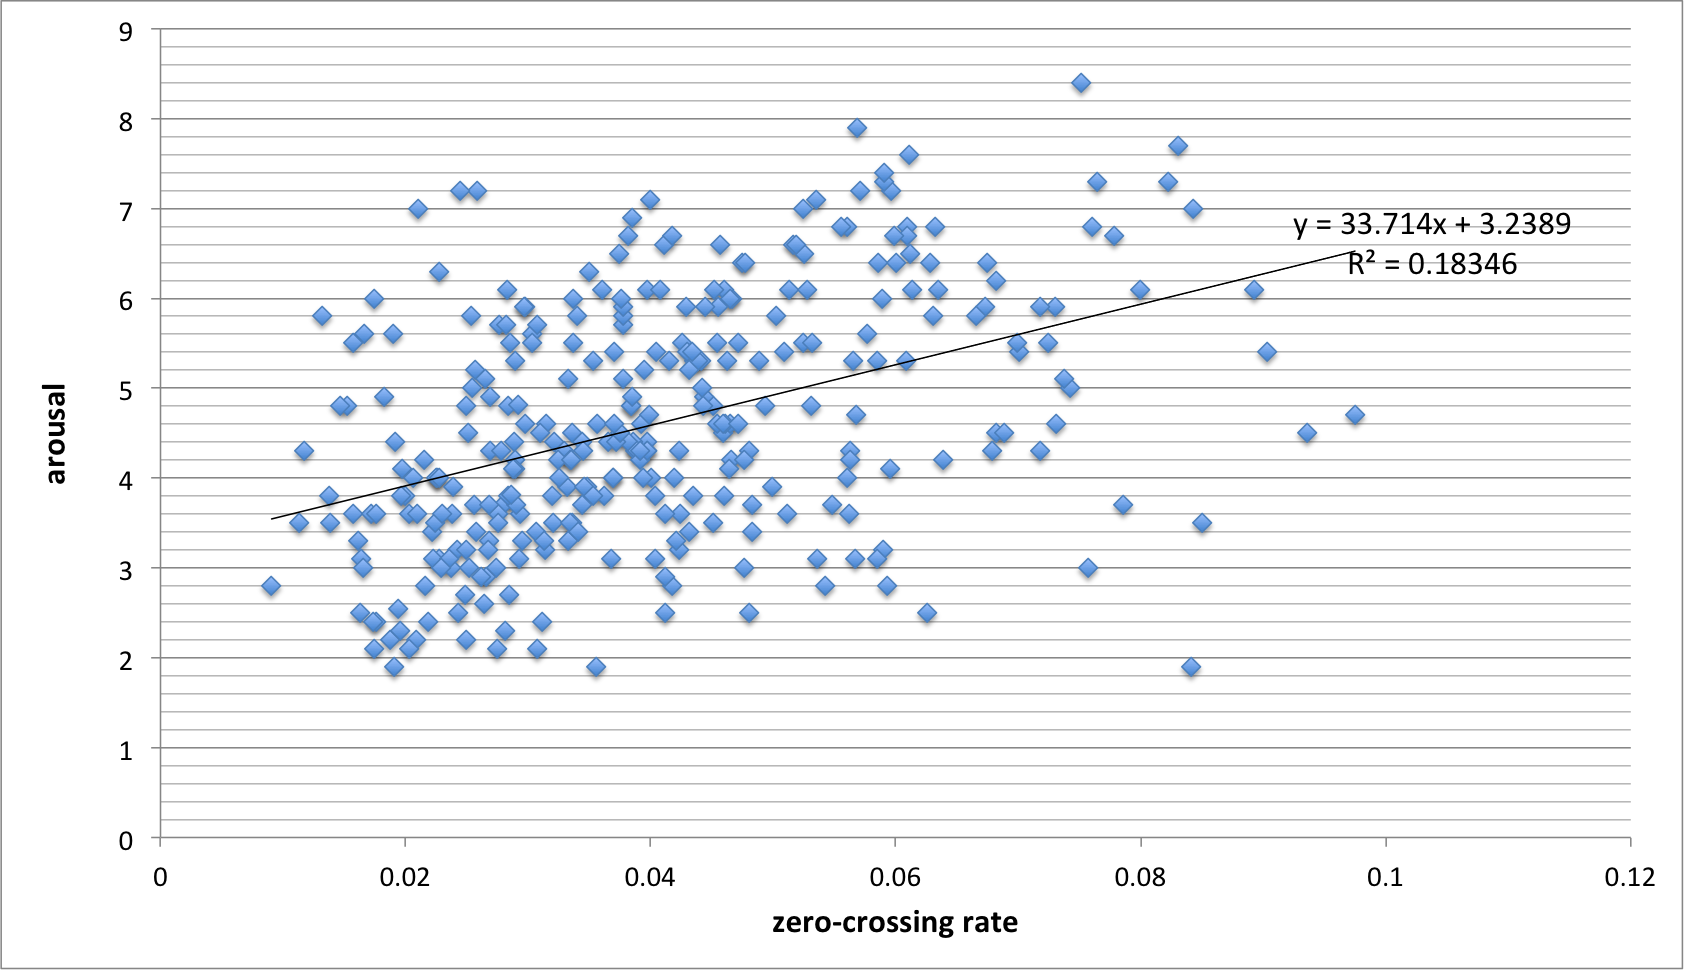
\includegraphics[width=\textwidth]{Figures/zerocrossing-arousal}
                \caption{A graph representing a correlation between zero-crossing rate and arousal values.}
        \end{subfigure}
          \caption{Chosen results of bivariate correlation with multiple regression.}
        ~ %add desired spacing between images, e. g. ~, \quad, \qquad, \hfill etc.
                        \label{fig:bivariateNN}

\end{figure}

\vspace{10pt}

\subsection{Correlation Between Features and Mood Perception}

In our exploration we decided to base our research on data collected in ``1000 Songs for Emotional Analysis of Music'' music library \cite{1000songs}, to avoid personal bias in assessing the mood of the song. The songs in the dataset were annotated by more than 300 crowdworkers on Amazon Mechanical Turk. Each song was annotated for arousal and for valence separately.

As a first step towards understanding the pattern by which audio features might account for emotion ratings, we conducted correlational analyses between features and mean valence/arousal ratings from the data set. We performed a bivariate correlation analysis with the valence/arousal ratings as the dependent variable, and each of the 22 features as the explanatory variable. Example of the results we achieved can be seen in Figure \ref{fig:bivariateNN}, the rest are included in Appendix A (Chapter \ref{AppendixA}, Section \ref{sec:bivariatediagram}) for reference. 

We found significant correlation between \textbf{valence} and derivative of variance and mean \textit{silence60}, derivative of variance of \textit{silence30, dynamic complexity, spectral centroid, spectral RMS, spectral energy, zero-crossing rate, pitch salience, and both mean and derivative of variance (dvar) of dissonance}. 

For \textbf{arousal}, we noticed correlation with \textit{spectral centroid, pitch salience, zero-crossing rate}, both \textit{mean} and \textit{dva}r of  \textit{silence60, spectral energy, mean dissonance} and \textit{dynamic complexity}. 

Values of all the features were then normalised between 0 and 1 to prepare them for the neural network training. 


\begin{wrapfigure}{l}{0.5\textwidth}
  \vspace{-30pt}
  \begin{center}
    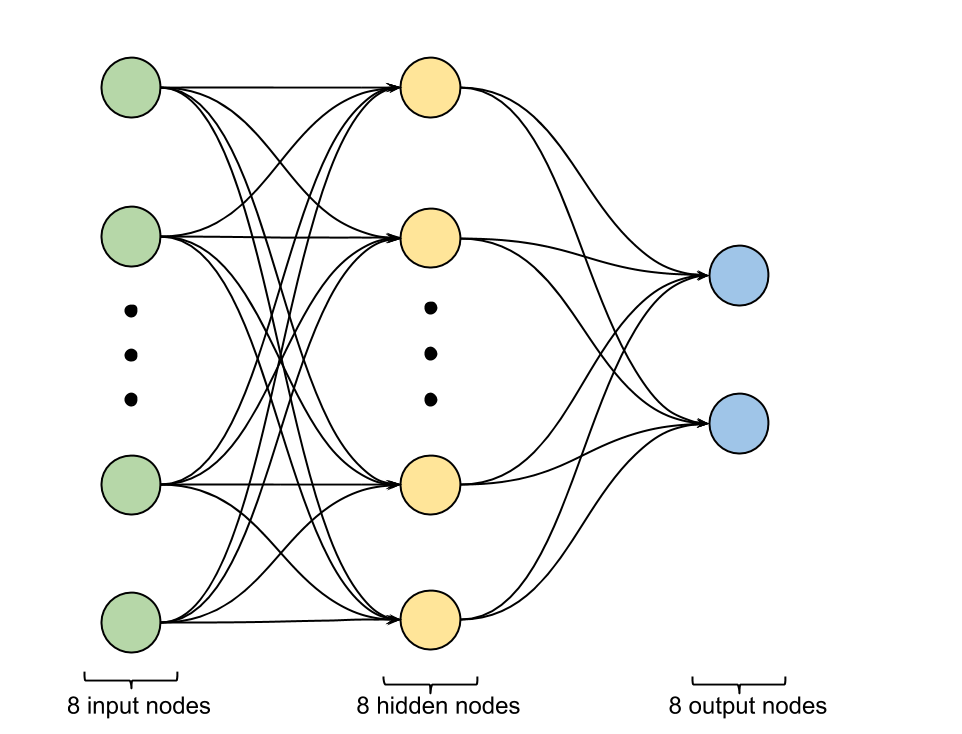
\includegraphics[width=0.5\textwidth]{Figures/myANN}
  \end{center}
  \caption{A diagram depicting the structure of our artificial neural network for mood detection.}
\label{fig:finalnetwork}
\end{wrapfigure}

\vspace{10pt}

\subsection{Neural Network for Mood Prediction}

Our goal was to train the network to predict mean participant valence and arousal values for musical excerpts. 
Our first network implementation was a supervised, feedforward network with backpropagation. 
The input consisted of normalised values of 8 features:
\textit{spectral centroid, pitch salience, zero-crossing rate, silence60 mean  and dvar, mean dissonance, dynamic complexity} and \textit{spectral energy}. 
The network had two outputs - arousal and valence.

As all the training data was normalised, the input and output values were within a range of 0 to 1. The training set consisted of 50 input and output arrays. Each input array had 8 values, one per audio feature, and its corresponding output array had the two desired arousal and valence values.

The network’s task was to provide the valence and arousal values based on the 13 audio features. The output values fell within a range of 0 to 1. Since desired outputs were average valence/arousal ratings provided by participants on a scale from 1 to 9, the network outputs were rescaled back. The training set consisted of eight input and output arrays. Each input array had 13 values, one for each audio feature, and its corresponding output array had the two desired arousal and valence values. The connection weights from input to the hidden nodes and from hidden nodes to the output ones were initialised to random numbers. 

The network was built, trained, and tested using the pyBrain python library for neural network implementation. 

We trained our network for 1000 epochs with many different sizes of the hidden layer and default values for all the other parameters. The performance based on that can be seen in Table \ref{table:rsmetable}.


Hidden neurons are the neurons that are neither in the input layer nor the output layer. Using additional layers of hidden neurons enables greater processing power and system flexibility at the cost of additional complexity in the training algorithm. Having too many hidden neurons can be thought of as a system of equations with more equations than there are free variables: the system is over specified and incapable of generalisation. Having too few hidden neurons, conversely, can prevent the system from properly fitting the input data, and reduces the robustness of the system.

\begin{figure}[h]
	\centering
   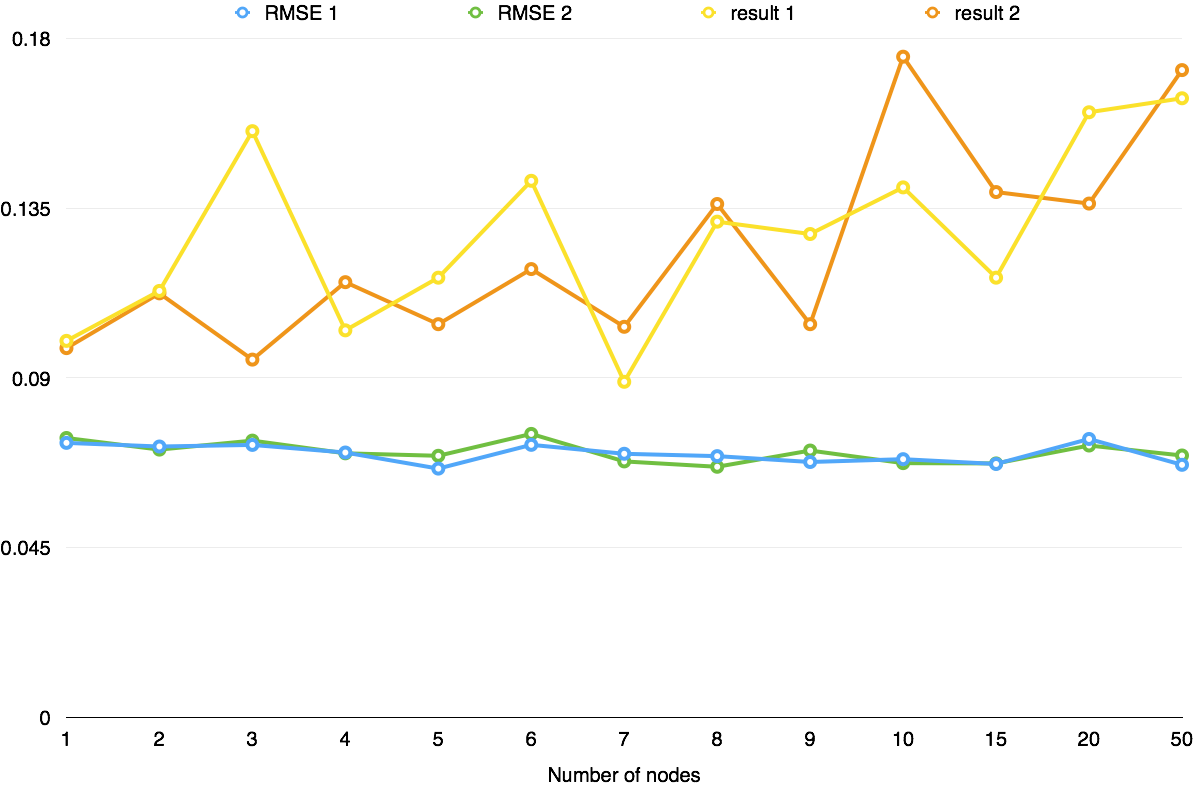
\includegraphics[width=0.7\textwidth]{Figures/nodesperf}
\caption{Data presented in table \ref{table:rsmetable}, plotted on a diagram.}
\end{figure}


\begin{table}
\begin{center}
\begin{tabular}{| c | l | l | l | l |} \hline 
  No. of Nodes & RMSE 1 & RMSE 2 & result 1 & result 2  \\ \hline \hline
  1 &  0.0727638005274 & 0.0740582536152  & 0.0998088934575 & 0.0978822145006 \\ \hline
  2 &  0.071796654024 & 0.0709793303052 & 0.113046836083 & 0.112405435125 \\ \hline
  3 & 0.0722212571658 & 0.0733605257262 &  0.155412522783 & 0.0948392717258 \\ \hline
  4 &   0.0702013899702 & 0.0699921976435 &  0.102602437509 & 0.115373051966 \\ \hline
  5 &  0.0659433293266 &  0.0693361162261 &  0.116558760273  & 0.10423200269\\ \hline
  6 & 	 0.0722427034758 & 0.0751383013205 &  0.142248432275  &  0.118843096333  \\ \hline
  7 &  0.0698701385354  & 0.0678483277007  & 0.088954243616 & 0.103537259056 \\ \hline
  8 &   0.0692459138916 &  0.066424019477 & 0.131412928439 & 0.136098090028 \\ \hline
  9 &   0.0676910853628 &  0.0707274913708 & 0.128139548772 & 0.104231713578\\ \hline
 10 & 0.0684398705278 & 0.0673887116962 & 0.140505458102 & 0.175156506583\\ \hline
 15 & 0.0671656450239 & 0.0673141803371 & 0.116563143115  &  0.139265837027\\ \hline
 20 & 0.0737978227013 &  0.0720620813131 & 0.160424096589 & 0.136210925296\\ \hline
 50 & 0.0669456166054 &   0.0694139442297 & 0.164132829293 & 0.171603556123\\ \hline
\end{tabular}
\caption{Table showing the root mean square error for training the network for given number of nodes in the hidden layer.}
\label{table:rsmetable}
\end{center}
\end{table}


As we can see, the optimal solution is the one with 7 nodes in the hidden layer. Although the initial RMSE returned after training is not overall minimum, all the values - so both the training ones and the ones after the evaluation, are local minimas and one of the minimal values overall. This decision can be justified by the fact that although for some cases we managed to achieve smaller RSME from the training, the network was in fact overfitting, and doing really well for the already known input, but worse for a new one.
To avoid overfitting the network, we kept the number of hidden units equal to the number of input units. 

\begin{table}
\begin{center}
\begin{tabular} {| c | l | l |} \hline
 Learning Rate & RMSE & result RMSE \\  \hline \hline
 0.3 & 0.0707970888752 & 0.14578838717 \\ \hline
 0.25 & 0.0699336891245 & 0.163193322998 \\ \hline
 0.2 &  0.0667986974361 & 0.15521882498 \\ \hline
 0.15 & 0.0724218948598 & 0.104971086068 \\ \hline
 0.1 & 0.0684257582616 & 0.100719004205 \\ \hline
 0.05 & 0.0695957657331 & 0.0979349713899 \\ \hline
 0.01 & 0.0689460348924 & 0.090954243616 \\ \hline
 0.005 & 0.0724023992534 & 0.130733683966 \\ \hline
 0.001 &  0.079664786995 & 0.112619882406 \\ \hline
\end{tabular}
\caption{Table showing the root mean square error for training the network for given learning rate parameter value.}
\label{table:learningrate}
\end{center}
\end{table}

\begin{figure}[h]
	\centering
   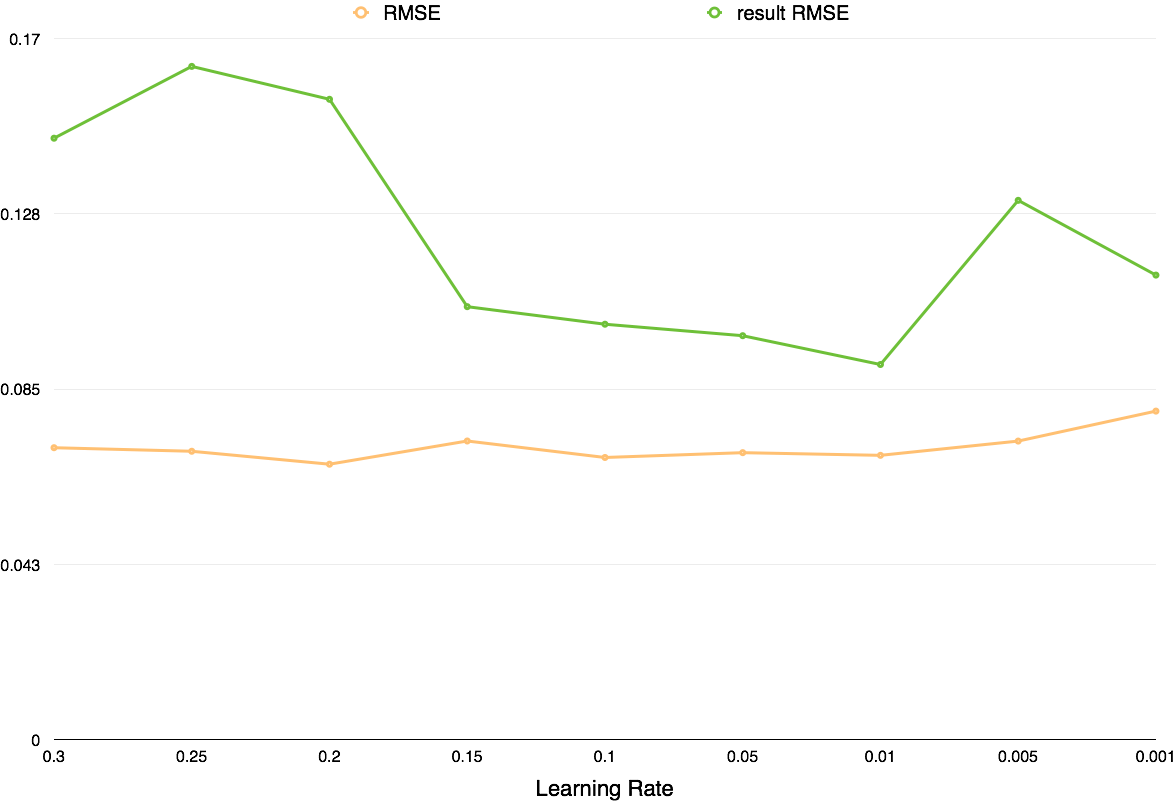
\includegraphics[width=0.7\textwidth]{Figures/learningrate}
\caption{Data presented in table \ref{table:learningrate}, plotted on a diagram.}
\end{figure}


Having found the optimal number of nodes in the hidden layer, we moved on to find the learning rate parameter. Training parameter that controls the size of weight and bias changes in learning of the training algorithm. In a standard backpropagation, too low a learning rate makes the network learn very slowly,whereas a learning rate that is too high makes the weights and objective function diverge, so there is no learning at all. 

We started our search by setting it to 0.3 and reducing it over time. The results we found can be found in Table \ref{table:learningrate}. As we can see, the optimal solution seems to be learning rate at value 0.001.


In the end, we came up with the network which can be seen on Figure \ref{fig:finalnetwork}.

\vspace{20pt}

\section{Main Melody Extraction}

\vspace{10pt}

\section{Structure Retrieval}

Understanding the structure of music (e.g. intro, verse, chorus, bridge, and outro) is important as it allows us to divide a song into semantically meaningful segments, within which musical characteristics are relatively consistent.

\vspace{10pt}

\subsection{Feature Choice}

To implement a system capable of unsupervised structure recognition, we need to provide it with some data. We investigated two possible values - \textit{Mel-frequency cepstral coefficients} and \textit{harmonic pitch class profile}.

Cepstrum is the result of taking the Inverse Fourier transform (IFT) of the logarithm of the estimated spectrum of a signal. It can be viewed as information about rate of change in the different spectrum bands.

The mel-frequency cepstrum (MFC) is a representation of the short-term power spectrum of a sound, based on a linear cosine transform of a log power spectrum on a nonlinear mel scale of frequency.

\textit{Mel-frequency cepstral coefficients} (MFCCs) are coefficients that collectively make up an MFC. They are increasingly finding uses in music information retrieval applications such as genre classification, audio similarity measures, etc.

MFCCs are derived from a type of cepstral representation of the audio clip. The mel-frequency cepstrum differs from cepstrum by having its frequency bands equally spaced on the mel scale, which approximates the human auditory system's response more closely than the linearly-spaced frequency bands used in the normal cepstrum. This frequency warping can allow for better representation of sound, for example, in audio compression.

MFCCs are commonly derived as follows:
\begin{itemize}
\item Take the Fourier transform of a signal.
\item Map the powers of the spectrum obtained above onto the mel scale, using triangular overlapping windows.
\item Take the logs of the powers at each of the mel frequencies.
\item Take the discrete cosine transform of the list of mel log powers, as if it were a signal.
\item The MFCCs are the amplitudes of the resulting spectrum.
\end{itemize}

An alternative to using MFCCs as the features to base the algorithm on is \textit{HPCP}.

Harmonic pitch class profiles (HPCP) is a vector of features extracted from an audio signal, based on the Pitch Class Profile descriptor. HPCP is an enhanced pitch distribution feature which is a sequence of chroma - feature vectors describing tonality measuring the relative intensity of each of the 12 pitch classes of the equal-tempered scale within an analysis frame. 

HPCP features can be found and used to estimate the key of a piece, to measure similarity between two musical pieces and to classify music in terms of composer, genre or mood. The process is related to time-frequency analysis. In general, chroma features are robust to noise, for example an ambient noise or percussive sounds, independent of timbre and instrumentation and independent of loudness and dynamics.

The General HPCP feature extraction procedure is summarised as follows:
\begin{itemize}
\item Input musical signal.
\item Do spectral analysis to obtain the frequency components of the music signal.
\item Use Fourier transform to convert the signal into a spectrogram. (The Fourier transform is a type of time-frequency analysis.)
\item Do frequency filtering. A frequency range of between 100 and 5000 Hz is used.
\item Do peak detection. Only the local maximum values of the spectrum are considered.
\item Do reference frequency computation procedure. Estimate the deviation with respect to 440 Hz.
\item Do Pitch class mapping with respect to the estimated reference frequency. This is a procedure for determining the pitch class value from frequency values. A weighting scheme with cosine function is used. It considers the presence of harmonic frequencies (harmonic summation procedure), taking account a total of 8 harmonics for each frequency. In order to map the value on a one-third of a semitone, the size of the pitch class distribution vectors has to be equal to 36.
\item Normalise the feature frame by frame dividing through the maximum value to eliminate dependency on global loudness.
\end{itemize}

The discussion of results given each of the alternatives are discussed in Section \ref{sec:structurefeatures}.

\vspace{10pt}

\subsection{Feature Preparation}

In this section, we will describe the process of preparation of the features for improving the performance of the algorithm. For simplicity and clarity, when talking about the features, we will first focus on analysis based on HPCPs, followed by one on MFCCs.
We decided to investigate both possibilities as they present the track from completely different perspective. For example, the HPCP chroma might fail to distinguish vocal and instrumental parts if the underlying harmonic patterns are exactly the same. On the other hand, when working with MFCCs we expect the opposite behaviour - good performance on parts that are different in terms of timbre.

\subsubsection*{Harmonic Pitch Class Profiles}

\begin{figure}
        \centering
        \begin{subfigure}[b]{0.47\textwidth}
                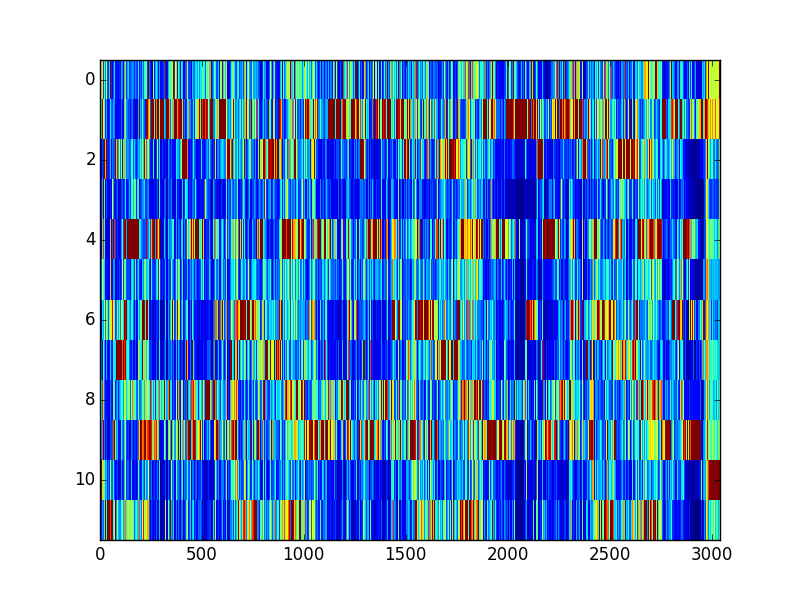
\includegraphics[width=\textwidth]{Figures/hpcp_unsynched_chroma}
                \caption{Example of a chromagram without any further enhancement. }
                \label{fig:unchroma}
        \end{subfigure}%
        ~ %add desired spacing between images, e. g. ~, \quad, \qquad, \hfill etc.
          %(or a blank line to force the subfigure onto a new line)
        \begin{subfigure}[b]{0.47\textwidth}
                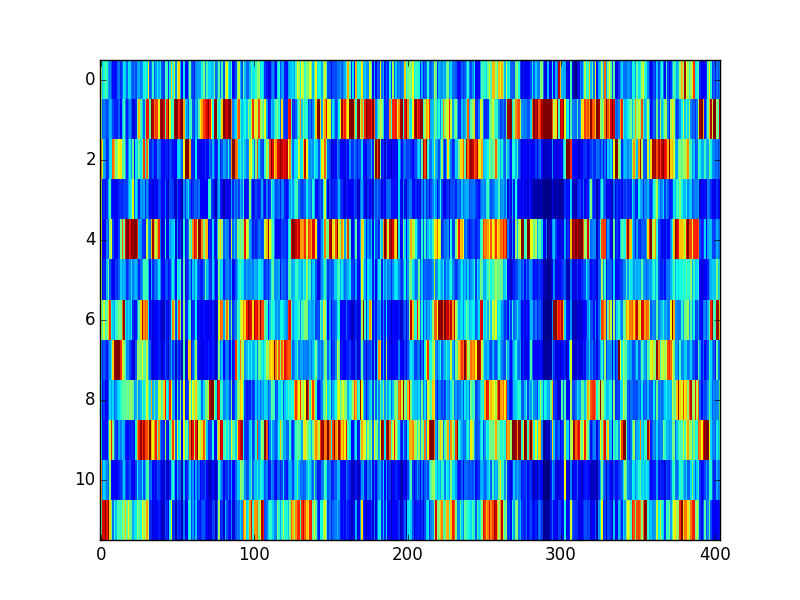
\includegraphics[width=\textwidth]{Figures/hpcp_synched_chroma}
                \caption{Example of a chromagram after beat-synchronisation.}
                \label{fig:synchroma}
        \end{subfigure}
          \caption{Harmonic pitch class profiles chroma features calculated for a song by The Beatles- ``Help!''.}
        \label{fig:chromacomparison}
\end{figure}

A series of transformations are applied to the data in order to distinguish the different parts of a song more efficiently with preserving the accuracy.. 

First, we need to we synchronise our data with the beats detected in the musical track. This process allows to reduce local variation by summarising (usually taking the mean or a median) frame-wise features that occur between two beats, yielding fewer but longer beat-synchronous frames. The rationale for doing so is that many features, such as chord labels that occur between two consecutive beats tend to be the same. Thanks to focusing on the values of the features on a per-beat basis, we manage to largely normalise variations in tempo. However, the main advantage of applying the beat-synchronisation is that we manage to reduce the amount of data to analyse, and hence, the size of the matrix, we are operating on.

This leads to beat-synchronous chromagrams. A diagram of a chromagram after beat synchronisation can be seen in Figure \ref{fig:synchroma}. As we can see, the size has decreased dramatically, which makes the segmentation process computationally cheaper.

\begin{figure}
        \centering
        \begin{subfigure}[b]{0.47\textwidth}
                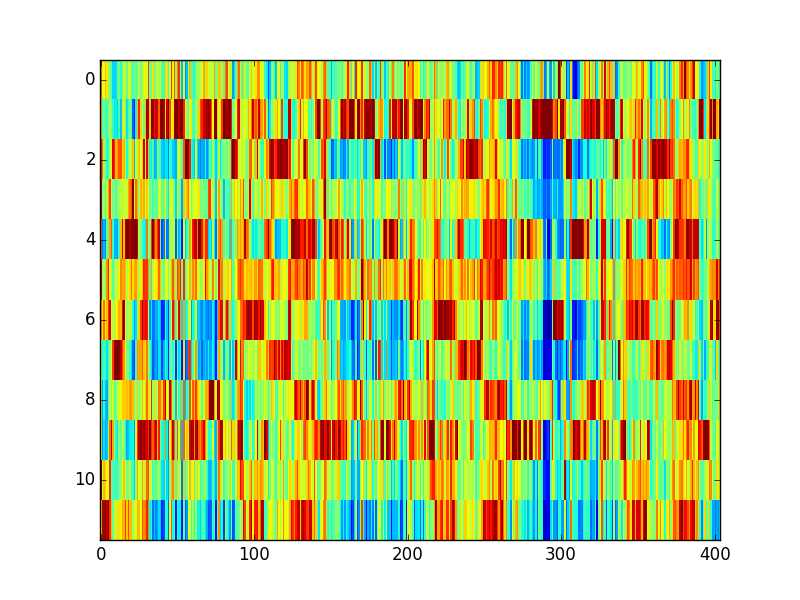
\includegraphics[width=\textwidth]{Figures/hpcp_synched_log_chroma}
                \caption{Chroma feature after applying log normalisation.}
                \label{fig:logchroma}
        \end{subfigure}%
        \begin{subfigure}[b]{0.47\textwidth}
                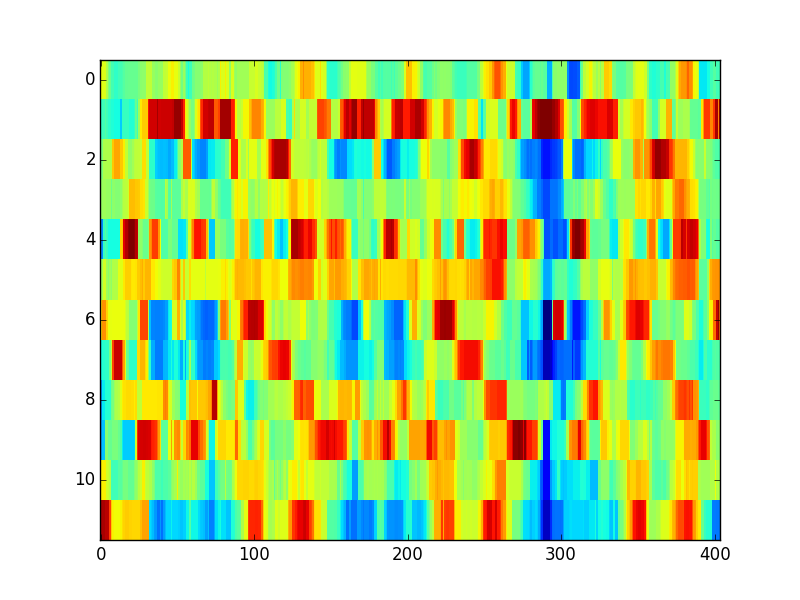
\includegraphics[width=\textwidth]{Figures/hpcp_synched_median_chroma}
                \caption{Chroma feature after applying sliding median filter of size h=9.}
                \label{fig:slidingchroma}
        \end{subfigure}
          \caption{Beat-synchronised chroma created for song ``Help!'' by The Beatles with applied enhancements.}
        \label{fig:chromaenhance}
\end{figure}

Following the beat-synchronisation, we apply log normalisation to the chroma feature. This allows us to reduce the effect the outliers from the trend will have and further improve the contrast between the related and unrelated beat frames. The enhancement achieved by applying log normalisation can be seen in Figure \ref{fig:logchroma}.

As the next step, we applied a sliding median filter of size h is run against each of the beat-synchronous and log-normalised chromagram channels, which can be seen in Figure \ref{fig:slidingchroma}. Thanks to the median filter, we can come up with sharper edges than with a regular mean filter. This becomes really useful in obtaining section boundary precision.

\begin{figure}
        \centering
        \begin{subfigure}[b]{0.47\textwidth}
                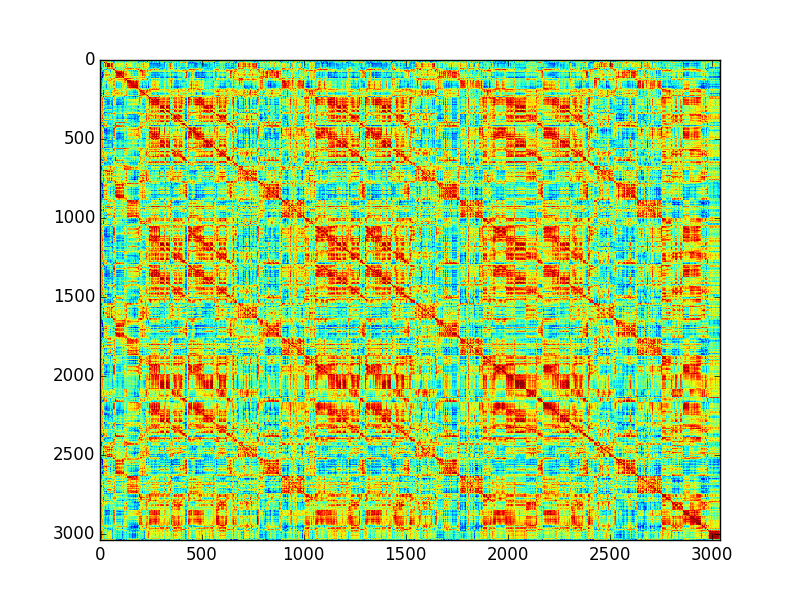
\includegraphics[width=\textwidth]{Figures/hpcp_unsynched_ssm}
                \caption{Similarity matrix generated from harmonic pitch class profiles chroma without further enhancement.}
                \label{fig:unSSM}
        \end{subfigure}%
        \begin{subfigure}[b]{0.47\textwidth}
                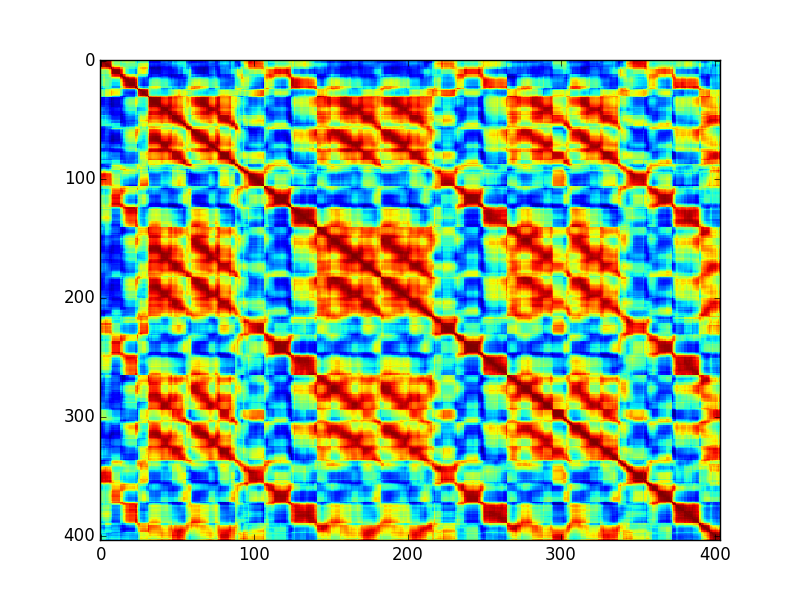
\includegraphics[width=\textwidth]{Figures/log_ssm_synched}
                \caption{Similarity matrix generated from beat-synchronised harmonic pitch class profiles chroma.}
                \label{fig:synSSM}
        \end{subfigure}
          \caption{Comparison of SSM generated from unprocessed and enhanced chromas, using correlation distance.}
        \label{fig:ssmcomparison}
\end{figure}

By filtering features across time, we retain the most prominent chromas within the h-size window and remove smaller artefacts, which are irrelevant in our con- text. The Figure \ref{fig:slidingmedian} presents the chromagram after applying the sliding median filter.

We then proceed to compute the Self Similarity Matrix (SSM) of the pre-filtered beat-synchronous chromagram. The SSM is essentially a pairwise comparison of a given set of features using a specific distance measure between the features of the two beat indices i and j. The result of every such comparison is stored in a N x N symmetric matrix D, such that D(i, j) contains said distance. In particular, D(i, j) stores the same value ad D(j, i), and for every i D(i, i) is equal to 0.

We investigated the influence of the type of the distance calculated on the SSM produced for the enhanced chroma. In our research we looked into four types of distance: euclidean, manhattan, correlation and cosine. Our results are presented in Figure \ref{fig:ssmdistance}. 
As we can see in Figures \ref{fig:euclidean} and \ref{fig:manhattan}, the contrast achieved is much weaker. Not only there are fewer blue spots signifying small or even no similarity between points, but the amount of points that are significantly similar is also reduced.


\begin{figure}[b]
        \centering
        \begin{subfigure}[b]{0.31\textwidth}
                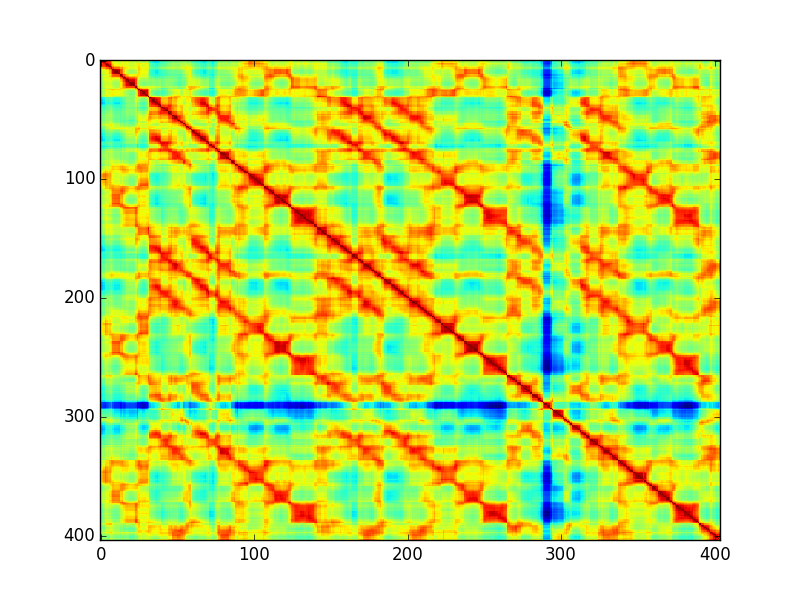
\includegraphics[width=\textwidth]{Figures/ssm_euclidean}
                \caption{Similarity matrix calculated from harmonic pitch class profiles chroma using Euclidean distance.}
                \label{fig:euclidean}
        \end{subfigure}%
        \begin{subfigure}[b]{0.31\textwidth}
                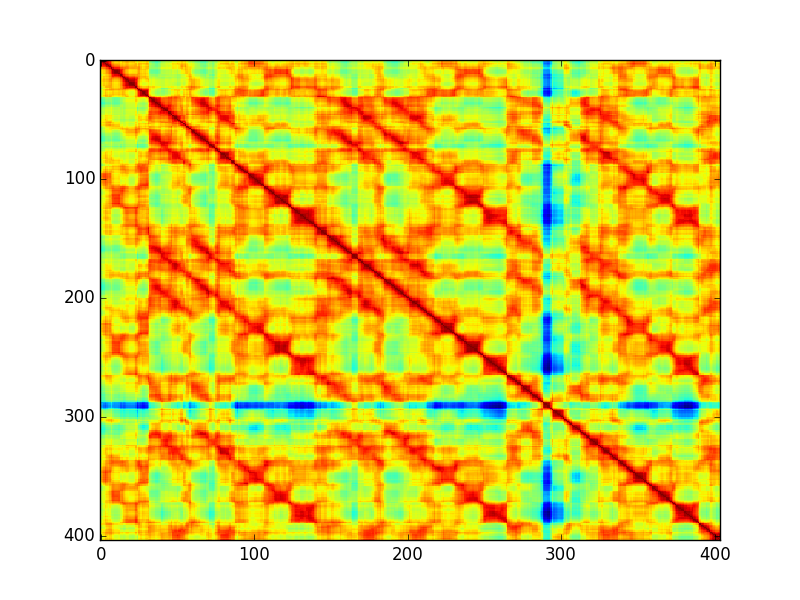
\includegraphics[width=\textwidth]{Figures/ssm_manhattan}
                \caption{Similarity matrix calculated from harmonic pitch class profiles chroma using Manhattan distance.}
                \label{fig:manhattan}
        \end{subfigure}
         \begin{subfigure}[b]{0.31\textwidth}
                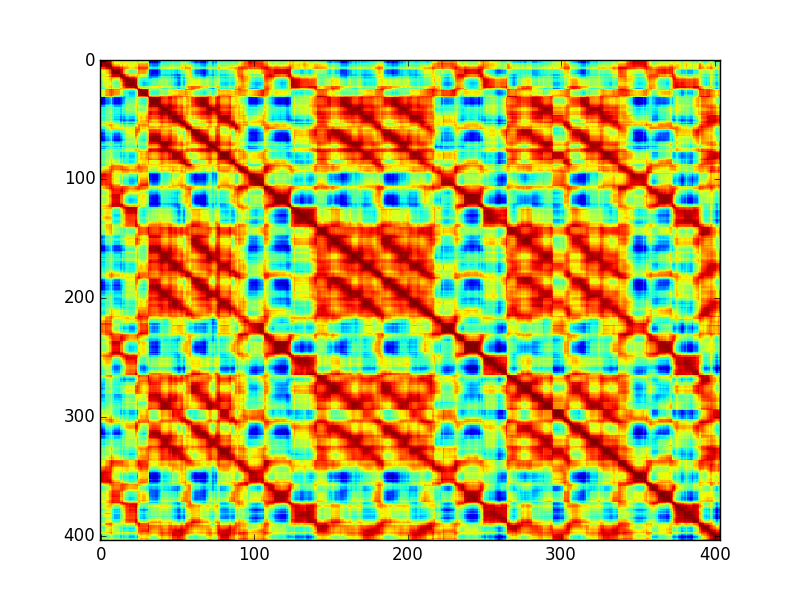
\includegraphics[width=\textwidth]{Figures/ssm_cosine}
                \caption{Similarity matrix calculated from harmonic pitch class profiles chroma using cosine distance.}
                \label{fig:cosine}
        \end{subfigure}
          \caption{Comparison of SSM computed using different distance formulas. The SSM calculated using correlation distance can be seen in Figure \ref{fig:synSSM}.}
        \label{fig:ssmdistance}
\end{figure}


When we look at the SSM computed using cosine distance, we can notice that the amount of the similar points has increased, more similar to the the one generated using the correlation distance. However, the correlation distance on Figure \ref{fig:synSSM} contains more dark blue spots, implying that it exposes more beats that are, in fact, not similar. This is why, in our design of the structure retrieval of a song we decided to use SSM computed using correlation distance.

\vspace{10pt}

\subsubsection*{Mel-frequency Cepstral Coefficients}

\begin{figure}
        \centering
        \begin{subfigure}[b]{0.47\textwidth}
                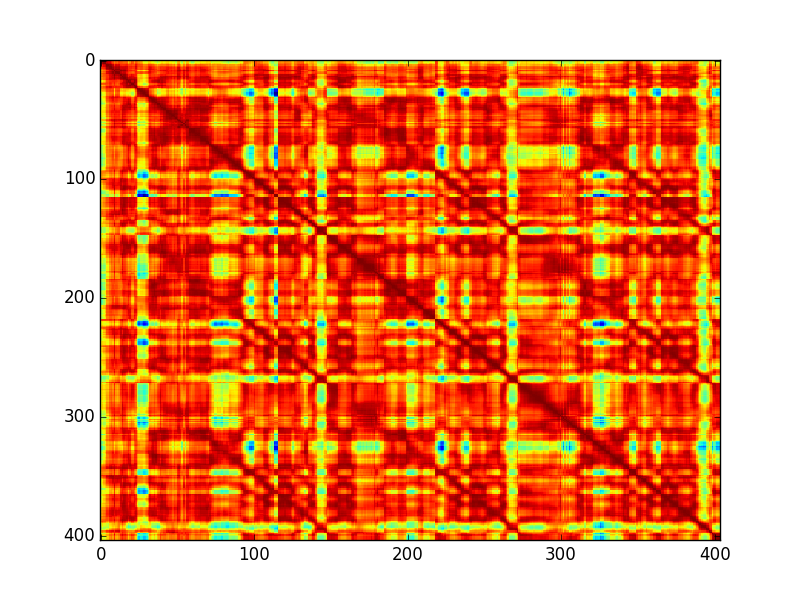
\includegraphics[width=\textwidth]{Figures/mfcc_no_log_sync}
                \caption{Similarity matrix generated from Mel-frequency Cepstral Coefficients without log normalisation.}
                \label{fig:unMFCC}
        \end{subfigure}%
        \begin{subfigure}[b]{0.47\textwidth}
                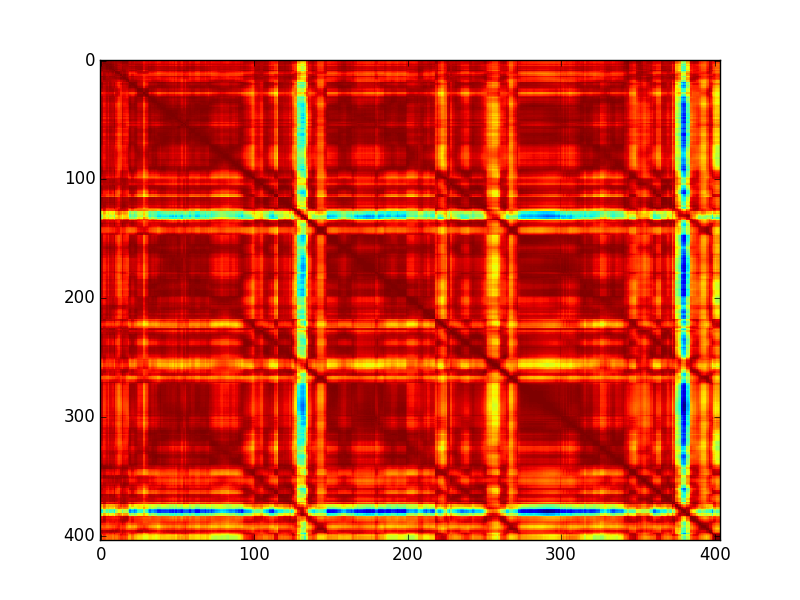
\includegraphics[width=\textwidth]{Figures/mfcc_ssm_synched}
                \caption{Similarity matrix generated from Mel-frequency Cepstral Coefficients with application of log normalisation.}
                \label{fig:synMFCC}
        \end{subfigure}
          \caption{Comparison of SSM generated from unprocessed and enhanced MFCCs, using correlation distance.}
        \label{fig:MFCCcomparison}
\end{figure}

Similarly to the case of Harmonic Pitch Class Profiles, we start the preparation of the features by beat-synchronisation to decrease the size of the data for further analysis. 

Now we have to determine whether log normalisation will improve the clarity of the SSM. As we can see in Figure \ref{fig:MFCCcomparison}, the use of log normalisation could decrease the amount of segments found, as more similar points are exposed.

Finally, we compute the SSM. Again, we investigated the possibility of generating it using Euclidean, Manhattan and cosine distances. The diagrams presenting our findings can be seen in Appendix B (\ref{AppendixB}). Similarly to when we were working with HPCPs, the correlation distance gave us the most contrasted, sharper images. 

The result of this process can be seen in Figure \ref{fig:synMFCC}.

\vspace{10pt}

\subsection{C-NMF}

We can view the SSM as an array of column vectors where each vector corresponds to a window. Suppose we have a set of vector templates. Vectors in the steady regions of a song may be directly found in the set, while vectors in the boundary regions may be approximated by linear combination of vector templates. Making this observation, we believe the Non-negative Matrix Factorization (NMF) could be useful in our situation.

\begin{wrapfigure}{l}{0.5\textwidth}
  \begin{center}
    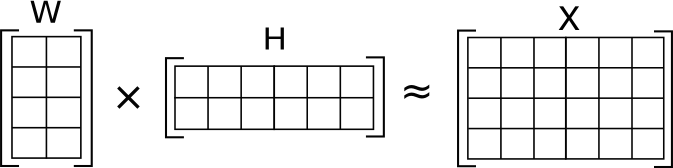
\includegraphics[width=0.45\textwidth]{Figures/NMF}
  \end{center}
  \caption{Illustration of approximate non-negative matrix factorization: the matrix X is represented by the two smaller matrices W and H.}
\label{fig:NMF}
\end{wrapfigure}

In NMF, the $N \times N$ self similarity matrix $X$ is approximately factorised into product of a $N \times k$ matrix $W$, can be interpreted as a cluster row matrix, and $k \times N$ matrix $H$, composed of the indicators of these clusters, where \textit{k} is the rank of the composition. This can be described as $X \approx WH$. The \textit{j}th column of $W$ can be viewed as the vector template for the \textit{i}th segment type. The \textit{j}th column of $H$ describes the intensities of the \textit{k}th segment types for the \textit{j}th window. In NMF, both $W$ and $H$ are enforced to be positive (i.e. $X$ must be positive too). We denote a row vector by $\boldsymbol{z}$ and a column one by $\boldsymbol{z}^{T}$.

However, in data mining, sometimes it can be beneficial to ensure X to contain meaningful “cluster centroids”, i.e., to restrict W to be convex combinations of data points.
C-NMF adds a constrain to $W$ = ($\boldsymbol{w}_{1}^{T}$, $\boldsymbol{w}_{2}^{T}$,... ,  $\boldsymbol{w}_{k}^{T}$),  such that its columns  $\boldsymbol{w}^{T}$  are, in fact,  convex combinations of the features of $X$:

\begin{equation}
\boldsymbol{w}_{j}^{T} = \boldsymbol{x}_{1}^{T}f_{1j} + \boldsymbol{x}_{2}^{T}f_{2j} + ... + \boldsymbol{x}_{N}^{T}f_{Nj}  \hspace{45pt}   j \in [1 : k]
\end{equation}

The linear combination is convex if all coefficients $f_{ij}$ are positive and the sum of each set of coefficients  $\boldsymbol{f}^{T}_{j}$ must be 1. Formally, this can be represented as:
$f_{ij} \geq 0,  f_{ij} = 1 $

This results in $W = XF$, where $F \in \mathbb{R}^{N \times k}$, which makes the rows $\boldsymbol{f}_{i}$ interpretable as weighted cluster centroids. The decomposition matrices $R_{j}$, are obtained as follows:  $R_{j} =  \boldsymbol{w}^{T}_{j}\boldsymbol{h}_{j}$, where $j \in [1 : k]$. Finally, C-NMF can be formally characterised as: $X \approx XFH$.

In C-NMF, the matrix W is a set of convex combinations of the rows of the input matrix X, which contrasts with NMF, where no such constraint exists. This means that, each row $x_{i}$ represents similarity of the time frame i with the rest of the time frames, storing information about the time frae i across the entire song.

By computing the C-NMF we separate basic structural parts. In the next sec- tion, we describe how the factorization via C-NMF relates to structure and show how we can use that result for music structure discovery.   ============ change ============

==== maybe try to get the plots of the decomposition matrices? =====

Apart from this, another important benefit of C-NMF over NMF is that matrices $F$ and $G$ become naturally sparse when adding the convex constrain. In case of NMF the $G$ does not always become sparse. Thanks to that, when using C-NMF we are more likely to find similar decomposition matrices for the same input than NMF, which is more sensitive to its initialisation \cite{Nieto}. 

\vspace{10pt}


\subsection{Boundaries}


\subsection*{K-means Clustering}

\begin{figure}[t]
        \centering
        \begin{subfigure}[b]{0.30\textwidth}
                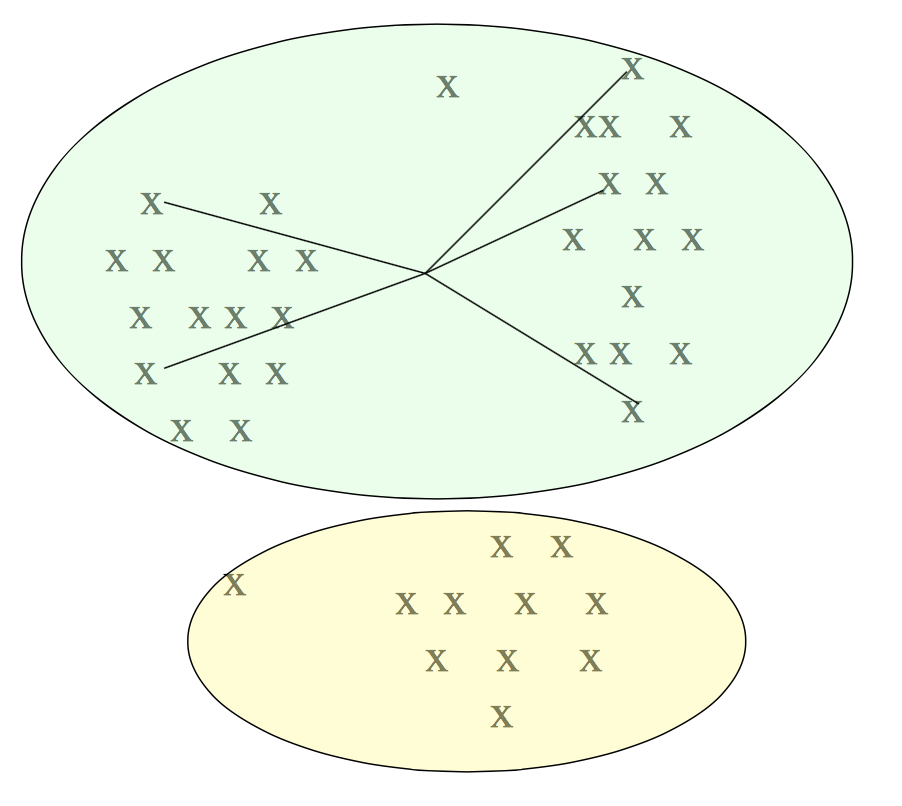
\includegraphics[width=\textwidth]{Figures/underfitting}
                \caption{The k value is too small - many long distances to centroids.}
                \label{fig:euclidean}
        \end{subfigure}%
        \begin{subfigure}[b]{0.30\textwidth}
                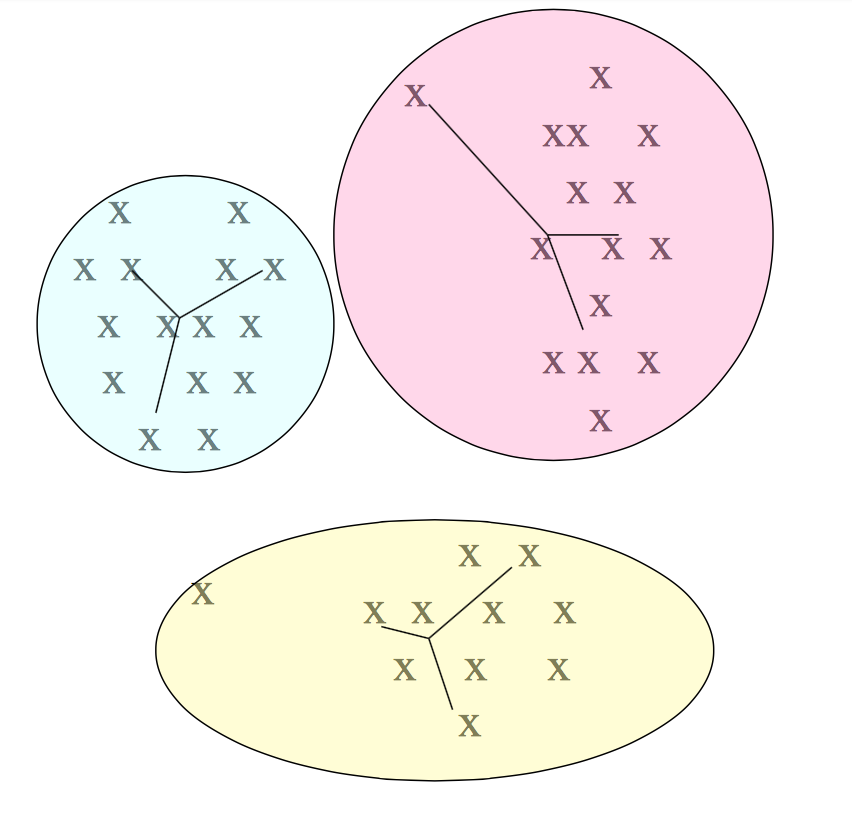
\includegraphics[width=\textwidth]{Figures/justright}
                \caption{Good k value - distances to centroids are quite short.}
                \label{fig:manhattan}
        \end{subfigure}
         \begin{subfigure}[b]{0.30\textwidth}
                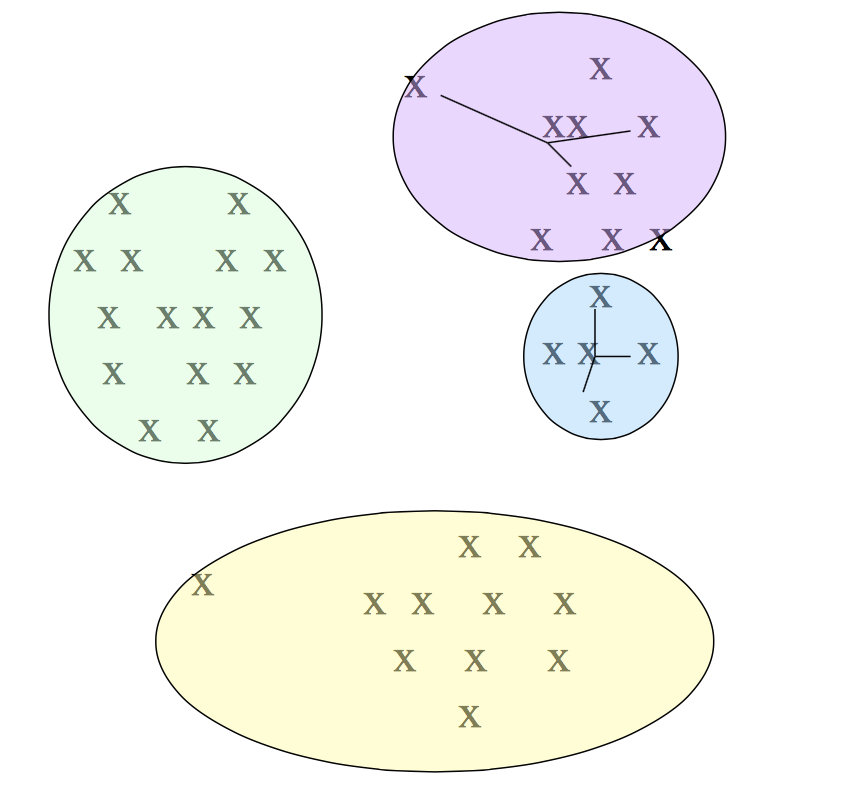
\includegraphics[width=\textwidth]{Figures/overfitting}
                \caption{The k value is too big - little improvement in average distance.}
                \label{fig:cosine}
        \end{subfigure}
          \caption{Diagrams depicting impact of the k value on the clustering result \cite{kcluster}.}
        \label{fig:ssmdistance}
\end{figure}

Clustering is an unsupervised classification of patterns, for example observations, data items, or feature vectors, into groups called clusters. The points within each cluster should be similar to each other and dissimilar to points belonging to another cluster. The problem has been addressed in many contexts and by researchers in many disciplines.

K-means clustering is considered one of the simplest unsupervised learning algorithms that can solve the well know clustering problem. It follows a simple and easy way of classifying a given data set through a certain number of clusters (assume k clusters).

The main idea  is to define k centres, one for each cluster. Much care should be put into their placement, as different location of centres causes different result. This is why the most intuitive solution is to put them as far apart as possible. The next step is to take one point after another from the data set and associate it with the nearest centre, 

When all the points have been assigned to some centre, k new centroids are calculated as baycentres of the clustering that resulted from the first phase. Once we have calculated the new centroids, a new binding has to be done  between the same data set points and the nearest new center. Very often this will result in points moving between different clusters. This can be considered second phase of the algorithms. 

Those two phases are repeated in a loop. As a result, we may notice that the k centers change their location step by step until no more changes are done, and the algorithm converges. 

We ran k-means clustering with k = 2 to each one of the C-NMF decomposition matrices, interpreting them as row-vector features. We efficiently obtained the section boundaries The choice of k = 2 allows us to detect boundaries (i.e. there’s a boundary or not), regardless of how the various sections cluster. However, after comparing the output of an this algorithm with a manually created segmentation, we noticed that k-means clustering's performance was not suited for our use. The granularity of the segmentation was too high - very often it separated parts of verse, or even fractions of seconds. Even after merging  values that were close together and getting rid of the smallest segments, the boundaries detected were too granular.


 
\vspace{10pt}

\subsection*{Another Approach}
Having applied the C-NMF, we computed, we have generated two decomposition matrices - $W$, called the cluster matrix, and $H$, an activation matrix, so that by multiplying them we can recreate the SSM, ie. $X \approx  WH$

\begin{figure}
        \centering
        \begin{subfigure}[b]{0.47\textwidth}
                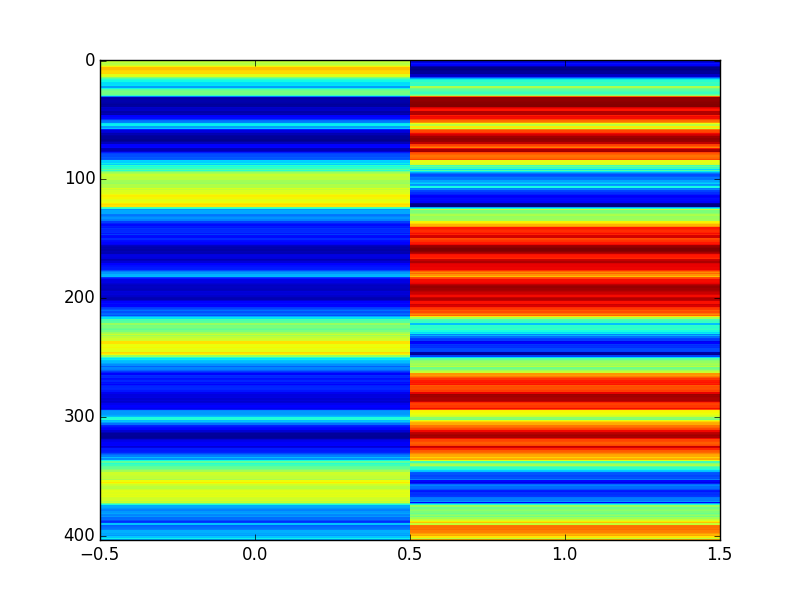
\includegraphics[width=\textwidth]{Figures/F}
                \caption{The cluster matrix W.}
                \label{fig:Wmatrix}
        \end{subfigure}%
        \begin{subfigure}[b]{0.47\textwidth}
                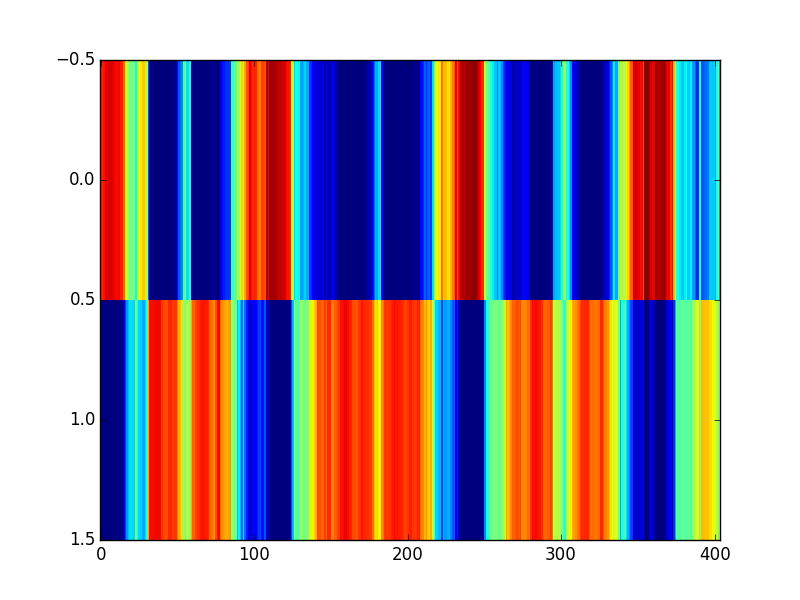
\includegraphics[width=\textwidth]{Figures/G}
                \caption{The activation matrix H.}
                \label{fig:Hmatrix}
        \end{subfigure}
          \caption{The result of C-NMF computed for ``Help!'' by The Beatles with rank k = 3.}
        \label{fig:CNMFbeatles}
\end{figure}


============ Once evaluating decide whether set k = 2 or not ===============        
        
To obtain the boundaries, we filter both the cluster matrix $W$ and the activation matrix $H$. This means that for every row corresponding to a frame in which the beat occurs, we find the indexes of the its maximum values. Thanks to this simple clustering, we obtain a assignment of each of the frames to one of the 'types' of segments. By iterating through a matrix generated and such ways and recording the indexes at which a song changes from one portion to another, we manage to obtain section boundaries in an efficient way. In our implementation, we start the computation with rank $k = 3$ and increase it if not enough bounds were found. This is to avoid overfitting and creating tiny segments, for example, one per verse line.

Once we have boundaries, we combine them within a distance window of size h so that boundaries close to each other get merged in their average location.


\subsection{Labelling}

In our structure retrieval, we investigated different ways of labelling of the segments.

First approach built directly on our way of segmenting the song.
Similarly to when attempting to find boundaries between segments, we decomposed our self similarity matrix X with rank increased. This allowed further differentiation between structures, for instance, if certain part of a song was thought of as a chorurs, but it is different enough to get separated in a C-NMF of a higher rank.

Once we have decomposed the matrix $X$, we filtered the clustering matrix $W$. This way, we computed initial clustering for each beat frame. To synchronise labels calculated in such way, we assigned a numerical label which occured within each of the interval between two segment to them.

However, having gathered data about the main melody of the song earlier on, we could use it to more accurately predict the labels for each of the song segments, producing labels that easy to understand to a person. In attempt to do so, we synchronise the array of pitches with the beats to get beat synchronised features which we could with ease refer to once we have the boundary frames. 

First intuition we had was to investigate the amount of silent frames occurring in each of the segments. After short investigation it was noticed, that, when reasoning about silences, as this approach performed better when frames with frequency 200 were treated as silent. 


\vspace{20pt}




\section{The Game}

In this section, we will go over the architecture and the design choices made when planning and implementing our game.

The game is written mostly in Swift, a multi-paradigm, compiled programming language created by Apple Inc. for iOS and OS X development. 
It was first introduced at Apple's 2014 Worldwide Developers Conference (WWDC). Swift is designed to work with Apple's Cocoa and Cocoa Touch frameworks, building on the best of C and Objective-C, without the constraints of C compatibility. It adopts safe programming patterns and adds modern features to make programming easier, more flexible, and more fun \cite{swiftintro}. 

We chose this language as we wanted to create a game for the OS X platform. In addition to this, the author also had a personal interest in learning the language.

\vspace{10pt}

\subsection{Data Storage}

The game relies on preserving user's scores and the levels generated by them. We need a way of storing them and all the information retrieved when analysing the songs to avoid regenerating the levels for the same song, for example if the user has a music piece they particularly like.

Core Data is the standard way to persist and manage data in both iPhone and Mac applications. It is an object graph and persistence framework provided by Apple in the Mac OS X and iOS operating systems. 

Core Data describes data with a high level data model expressed in terms of entities and their relationships plus fetch requests that retrieve entities meeting specific criteria. Code can retrieve and manipulate this data on a purely object level without having to worry about the details of storage and retrieval. 

Core Data allows data organised by the relational entity–attribute model to be serialised into XML, binary, or SQLite stores.

Core Data is also a persistent technology, in that it can persist the state of the model objects to disk. But the important takeaway is that Core Data is much more than just a framework to load and save data - it is also about working with the data while it is in memory.
We decided to use Core Data rather than a separate database as our game only needs to store data used by the current user, that will be utilised almost immediately after loading into memory. 
  
The model might cause some intensive memory usage if we decide to create a big amount of users, however, as it is an offline game that can be played on a personal machine, in contrast to web application, the number of users should remain relatively small.

\vspace{10pt}

\subsection{Menu}

Although not usually adopted in OS X games, we decided to follow the Model-View-Controller design pattern in implementing our application. We believe it was a right choice as the complexity of the main menu would have to be then supported throughout the played level. This would not only be a performance strain, but would also cause the code to be messy.

When first facing the menu, the user has an option of creating an account, logging in as a user or playing a quick game, not requiring any user data. 
The quick game is essentially an ability of playing one of the predefined levels, without a choice of creating a new one.

Once the user has created an account or chosen an existing one, they can either follow the level creation or level loading option. If they choose to create a new level, they have to select a file from their hard drive they would like to use as the base for their level. Otherwise, they go to the window, where they can select a level and either play it or remove it from their catalogue.

\vspace{10pt}

\subsection{Level Description}

Once we move on to playing a game, the \verb|GameViewController| unpacks the \verb|GameScene| - an object representing a scene of content in Sprite Kit.

Sprite Kit provides a graphics rendering and animation infrastructure that can be used to animate arbitrary textured images, or sprites. It uses a traditional rendering loop where the contents of each frame are processed before the frame is rendered. Its advantage is that it was developed for Apple hardware, hence it is optimised to render frames of animation efficiently using the graphics hardware. Thanks to this, the positions of sprites can be changed arbitrarily in each frame of animation. Sprite Kit also provides other functionality that is useful for games, including basic sound playback support and physics simulation. \cite{spritekit}. 

In the game scene, there is a set of buttons at the bottom of the screen. Players use the strum bar along with the fret buttons to play notes that scroll down the screen. The Easy difficulty only uses the first three fret buttons, that is, the green, red, and yellow. The Medium difficulty uses the blue button in addition to those three, and Hard and Expert use all five buttons.

The score is calculated based on how many scrolling notes we manage to hit. Every time we hit, the performance bar on the right side of the screen goes up, otherwise it goes down. If it hits the minimum, it the player loses. However, if the player manages to keep the performance level at the maximum for an appropriate amount of time, the number of the points scored for the new notes gets doubled until he misses a note or wins the level.

The player can at any time pause, stop or replay the game. They can also control the volume of the music and other sounds in the game. 

Upon completion of the level the player presented with their score, shown as stars and a concrete number. The player can later revisit the levels if they want to improve their score. 

\vspace{10pt}

\subsection{Melody Detection as a Game Changer}

The main part of the gameplay relies on the user pressing buttons that line up on the screen. As this is a music game, there are various ways of making the process more intuitive and hence attractive to potential players. 

One of the possibilities is to use the main melody of the song to determine which buttons to issue for the player by tying in the melody extraction.


...

Having processed the list of pitches in such way, we have prepared the ground for the buttons generation.

The main idea of the game is to mimic the playing an instrument on the computer keyboard. For this purpose we looked to 2 most popular instruments - guitar and piano for inspiration. 

When playing the piano, we are presented with a set of keys. 

\vspace{10pt}

\subsection{Introduction of The Song Segmentation}

\vspace{10pt}

\subsection{Impact of the Mood on the Level}

\vspace{20pt}


\section{Main Section 2}

% Evaluation

\chapter{Results and Evaluation} % Main chapter title

\label{Chapter6} % For referencing the chapter elsewhere, use \ref{Chapter4} 

\lhead{Chapter 6. \emph{Results \& Evaluation}} % This is for the header on each page - perhaps a shortened title

%----------------------------------------------------------------------------------------

Success of any project or product depends on many factors - the performance, design, innovation and design. Each of the elements it consists of contribute to at least one of them. 
In this chapter we evaluate our project in attempt to assess its success.

First, we focus on quantitative analysis. We present the results of testing and validating of our neural network for music emotion prediction using fresh and unseen data and contrast them with existing literature. Then we move on to evaluation of the boundary detection system by comparing the performance and accuracy it yields with two other algorithms. Finally, we examine the results of the labelling algorithm.

Last, but not least, we move on to user experience research. We go over user testing and its outcome, as well as how it was used to further improve our game. 

\vspace{10pt}

\section{Evaluation of Mood Detection system}

\begin{figure}[t]
    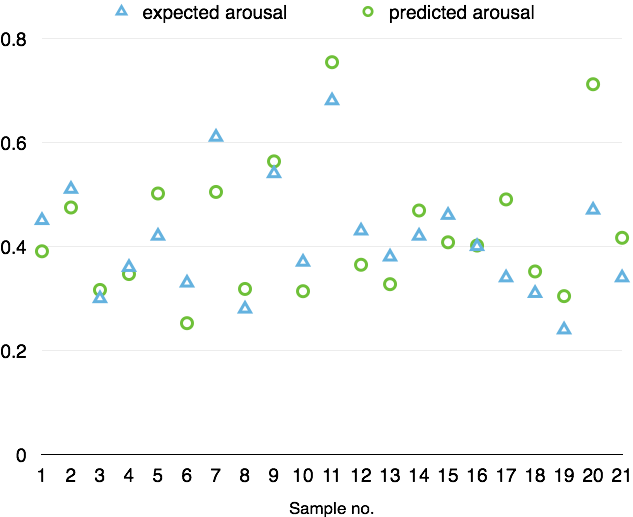
\includegraphics[width=0.7\textwidth]{Figures/finalarousal}
    \centering

  \caption{A plot of the expected and predicted .}
  \label{fig:anneval}
\end{figure}


We designed our neural networks to as means of calculating valence and arousal ratings of songs using audio features we extract. 

To evaluate its performance we have to have a way of telling how successful it is in guessing the values. To achieve this, we activated the network on 21 unseen music tracks that we knew valence and arousal values of and gathered the output network produced for it. Then, we computed the root mean square error between the ground truth ratings and network-predicted outputs across all segments of all the test melodies. The network's performance total RMSE was 0.08895 on scale from 0 to 1 or 9\%. The plot of the expected and predicted values can be seen in Figure \ref{fig:anneval}.

In contrast, in their paper \cite{vempala} Vempala and Russo trained a neural network with 1.14 error on scale 1 to 9, or 14.3\%.

If we look at the two predicted values separately, the coefficient of determination for the arousal reached 59.24\% and 40.34\% for valence.

In comparison, Yang and Lin \cite{mood} achieved a lower success rate, as their $R^2$ scored 58.3\% for arousal and 28.1\% for valence. 


\begin{figure}[t]
    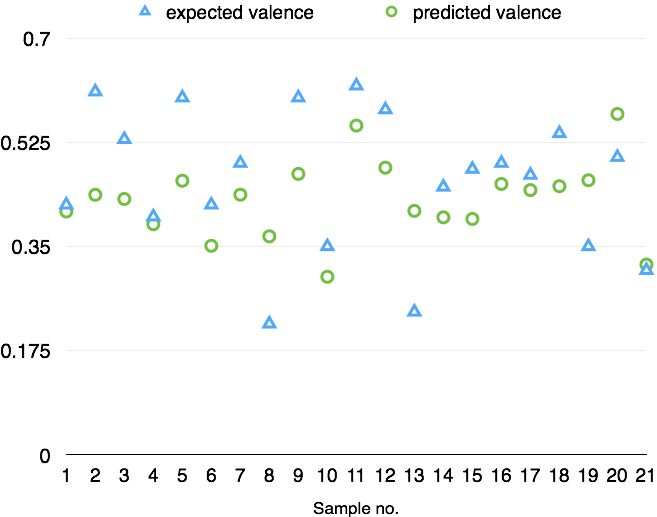
\includegraphics[width=0.7\textwidth]{Figures/finalvalence}
    \centering

  \caption{A plot of the expected and predicted valence.}
  \label{fig:anneval}
\end{figure}


Results from the static network indicate that a network can be trained to identify statistical consistencies across audio features abstracted from music and satisfactorily predict valence/arousal values that closely match mean participant ratings.


\begin{table}
\begin{center}
\begin{tabular}{| c | c | c | c | } \hline 
 expected arousal & expected valence & predicted arousal & predicted valence \\ \hline \hline

0.45  & 	0.42  &  0.390444 &  0.408524   \\ \hline
0.51	&  0.61  &  0.474538 & 0.436625   \\ \hline
0.3    &  0.53  &  0.316230 & 0.429643   \\ \hline
0.36	&  0.4    &  0.346713 & 0.387249   \\ \hline
0.42	&  0.6    &  0.501414 & 0.460295   \\ \hline
0.33	&  0.42  &  0.252398 & 0.350910  \\ \hline
0.61	&  0.49  &  0.504392 & 0.436785   \\ \hline
0.28	&  0.22  &  0.318096 & 0.366836   \\ \hline
0.54	&  0.6    &  0.563120 & 0.471717   \\ \hline
0.37	&  0.35  &  0.313782 & 0.298909   \\ \hline
0.68  &  0.62  &  0.753534 & 0.552922   \\ \hline
0.43	&  0.58  &  0.364568 & 0.482194   \\ \hline
0.38	&  0.24  &  0.327288 & 0.409628   \\ \hline
0.42  &  0.45  &  0.468762 & 0.398749   \\ \hline
0.46  &  0.48  &  0.407701 & 0.396029   \\ \hline
0.4    &  0.49  &  0.401469 & 0.454892   \\ \hline
0.34  &  0.47  &  0.490065 & 0.444592   \\ \hline
0.31  &  0.54  &  0.351714 & 0.451086   \\ \hline
0.24  &  0.35  &  0.304314 & 0.461078   \\ \hline
0.47	&  0.5    &  0.711224 & 0.572459   \\ \hline
0.34	&  0.31  &  0.416320 & 0.319491   \\ \hline
\end{tabular}
\caption{Table showing the root mean square error for training the network for given number of nodes in the hidden layer.}
\label{table:rsmetablefinal}
\end{center}
\end{table}



\section{Boundary Detection}

The first towards the evaluation of the segmentation algorithm was to gather the ground truth data to test against. To remove bias caused by personal preferences in music, we sought external sources for help in selection of the tracks. This is why we consulted the top charts created by music magazines and online portals such as Rolling Stone, Billboard, Gibson etc. The full list can be found in \cite{toplists}.

Once we have retrieved the lists with the most popular songs across genres, we selected one song per top list based on our familiarity. Although this might introduced some sort of personal preference into the dataset, it also allowed us to more intuitively create the ground truth data, as the familiarity with a song makes the manual labelling more obvious. For instance, in “Blitzkrieg Bop” by The Ramones, the bridge is repeates as often as verse and chorus, which is bound to introduce confusion to a person who hears the song for the first time and is asked to segment and label it.

In totall, we manually labelled 10 songs:
\vspace{-10pt}
\begin{description}
\itemsep0em 
\item[“The Number of The Beast”] by Iron Maiden (Metal)
\item[“Rock With You”] by Michael Jackson (Soul/R\& B)
\item[“Blitzkrieg Bop”] by The Ramones (Punk Rock)
\item[“This Land is Your Land“] by Woody Guthrie (Folk)
\item[“One More Time”] by Daft Punk (Dance)
\item[“Smooth”] by Santana (featuring Rob Thomas) (Pop)
\item[ “Crazy in Love”] by Beyonce (featuring Jay-Z) (Pop / Rap)
\item["Help!"] by The Beatles (Rock)
\item["Respect"] by Aretha Franklin (R\& B)
\item["Back in the USSR"] by The Beatles (Rock)
\end{description}

For each of the songs, we conducted 5 measurements to manually detect the boundaries. Once we have gathered the data, we averages each bound to create ground truth with reference boundaries and labels.

To be able to fully evaluate the performance of our algorithm in comparison with state-of-the-art solutions already existing, we also gathered data produced by two other algorithms. The first one, described by Foote and Cooper \cite{FooteCooper}, is a classic approach applying a "“checkerboard” kernel over the diagonal of a self similarity-matrix (SSM). The other one is an approach published by Kaiser and Sikora \cite{Sikora}, with use of non-negative matrix factorisation on only one feature. 

We conducted two types of studies to determine the performance of our bound finding algorithm.

First and the most intuitive one is the comparison of amount of boundaries detected. If an algorithm returns a smaller amount of segments it means that most probably its detection system is not sensitive enough - it merges some of bounds into bigger ones. And vice versa - if the algorithm returns more boundaries than the ground truth, it means it picked on song segments that differ in a less obvious way and, hence, its output is too granular.


\begin{table}
\begin{center}
\begin{tabular}{| c | c | c | c | c | } \hline 
Song  								& Ground	& Foote 	&  Kaiser 	& Ours \\ \hline \hline
The Number of The Beast 	&	17			& 	9  			&  15 		&  20   	\\ \hline
Rock With You					&	11			&  9			&  15 		& 17   	\\ \hline
Blitzkrieg Bop 					&	14			&  9  			&  14 		& 14   	\\ \hline
This Land Is Your Land 		&	11			&  9			&  12 		& 7    	\\ \hline
One More Time					&	13			&  9    		&  14 		& 17   	\\ \hline
Smooth								&	14			&  9  			&  14 		& 16  	\\ \hline
Crazy In Love					&	17			&  9  			&  13  		& 16   	\\ \hline
Help!									&	10			&  9		   	&  17 		& 12   	\\ \hline
Respect								&	12			&  9  			&  14 		& 12  	\\ \hline
Back In the USSR				&	15			&  9  			&  13		    	& 14		\\ \hline \hline
RMSE								&	N/A		& 4.98		&  3.08		& 2.95	\\ \hline 

\end{tabular}
\caption{Table showing the root mean square error for training the network for given number of nodes in the hidden layer for the checkerboard algorithm (by Foote, \cite{FooteCooper}), NMF based algorithm (by Kaiser, \cite{Sikora}) and ours.}
\label{table:evalStructureCount}
\end{center}
\end{table}


The results of our investigation can be seen in Table \ref{table:evalStructureCount}. By calculating the root mean square error for outputs of every algorithm, we noticed that our algorithm has a slightly better performance than the simple non-negative matrix factorisation one. On the other hand, checkerboard designed by Foote and Cooper consistently returned 9 labels, and hence yielding the worst performance.

Apart from observing the RMSE of the boundary number, we reasoned about the distribution of the results. In particular, we believe that the situation when the algorithm is over-segmenting, returning more bounds than there are in the ground truth, is better than the one when the structure retrieval system is not sensitive enough and merges boundaries that do not belong together. This is especially true in case of our application, where if more boundaries are returned, the mood detection becomes more accurate at expense of efficiency. On the other hand, with every lost bound we lose precision in the mood detection in two neighbouring segments.

If we look at Figure \ref{fig:boundcount}, we can see that in the light of our previous observations, the checkerboard yields a dramatically worse performance than nmf and our algorithm. In contrast, the latter two exhibit the same proportion of over- and under-segmenting.


\begin{table}
\begin{center}
\begin{tabular}{| c | c | c | c | c | } \hline 
Song  								& 	500ms 			&  3s						&  deviation	\\ \hline \hline
The Number of The Beast 	&	Foote			& 	Foote  				&  Ours 			\\ \hline
Rock With You					&	Ours				&  Ours			  		&  Ours			\\ \hline
Blitzkrieg Bop 					&	Kaiser			&  Ours  				&  Ours 			\\ \hline
This Land Is Your Land 		&	Ours				&  Foote			  	&  Foote 		\\ \hline
One More Time					&	Foote			&  Foote    				&  Ours 			\\ \hline
Smooth								&	Foote			&  Foote  				&  Ours 			\\ \hline
Crazy In Love					&	Ours				&  Ours  				&  Ours  		\\ \hline
Help!									&	Ours				&  Foote		   		&  Ours 			\\ \hline
Respect								&	Foote			&  Ours  				&  Ours 			\\ \hline
Back In the USSR				&	Ours/Kaiser	&  Ours/Kaiser 		&  Ours		    	\\ \hline

\end{tabular}
\caption{Table showing the best performing algorithm in each category for all the songs.}
\label{table:evalStructureRank}
\end{center}
\end{table}


\begin{wrapfigure}{r}{0.5\textwidth}
\vspace{-10pt}
  \begin{center}
    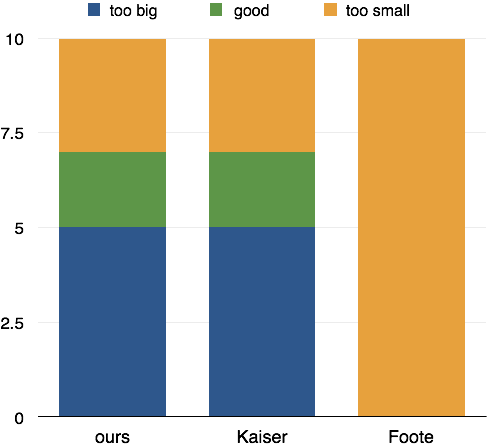
\includegraphics[width=0.48\textwidth]{Figures/count}
  \end{center}
  \caption{Figure presenting the amount of each type of errors produced by all the evaluated algorithms.}
\label{fig:boundcount}
\end{wrapfigure}

Another measurement of success of our boundary retrieval is computation of boundary detection hit-rate. A hit is counted whenever a reference boundary is within a certain window of an estimated boundary. An important thing to note is that each boundary should be matched at most once, otherwise we can get some irrelevant results. For instance, if we are estimating the algorithm with window size 3 seconds, in the ground truth there are two boundaries 6 seconds apart and our algorithm detects only one right in the middle, if we do not exclude the boundary once compared with the first one in the ground truth, the performance of our algorithm will be ranked as much better than it actually was. 


In addition to computing the hit-rate for windows of sizes 500ms and 3s, we also computed the median deviations between the reference and estimated boundaries of the song. In particular, we focused on median time from each reference boundary to the closest estimated boundary.

We implemented our evaluation benchmark using Python mir\textunderscore eval library \cite{mireval}.
Again, to best evaluate performance of our algorithm, we compare the results it yields with results of the checkerboard and NFM based ones. Our findings can be seen in Table \ref{table:evalStructureRank}.


\begin{wrapfigure}{r}{0.5\textwidth}
\vspace{-30pt}
  \begin{center}
    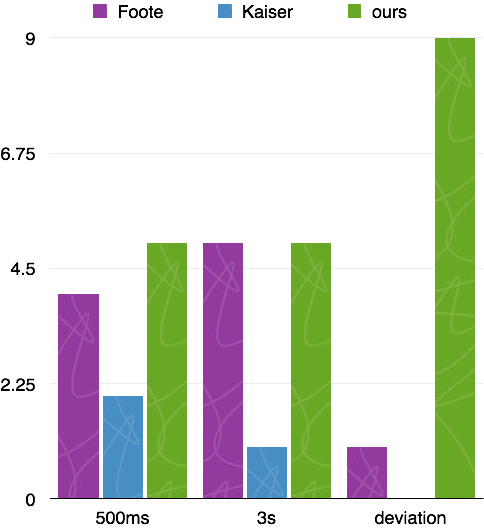
\includegraphics[width=0.48\textwidth]{Figures/structurechamps}
  \end{center}
  \caption{Chart presenting amount of times every algorithm excelled in each of the categories - hit-rate with window sizes of 500ms and 3s and the median deviation from the ground truth.}
\label{fig:structurechamps}
\end{wrapfigure}

As we can see in the Figure \ref{fig:structurechamps}, in the majority of cases, the performance of the algorithm designed by Kaiser falls behind the other two methods. It ranked as first twice when calculating the hit-rate with the window size w=500ms, once for the w=3s and it never excelled in the deviation category. On the other hand, the algorithm designed by Foote and Cooper yields similar overall performance as ours when evaluating hit-rate with w=3 and slightly worse for 500ms. This most probably is caused by the fact that in many cases our algorithm managed to find the segments but was a bit off, not qualifying for the 500s window. However, once the window got increased, its performance improved more than in case of the ``checkerboard'' algorithm. The exact results can be seen in section \ref{sec:segevalapp} in Appendix C. 

In conclusion, we believe that the algorithm for boundary detection we created is suitable for our application and yields performance comparable or exceeding the state-of-the-art creations in its field. 

\section{Labelling}


\section{Questionnaires}
Questionnaires are one of the most common and popular tools to gather data from a large number of people. They generally consist of a limited number of questions that ask participants to rate the effectiveness of various aspects of the activity. The questions should focus on the key points we are trying to evaluate. 

Questionnaires tend to be short in order to reduce the amount of time respondents need to complete them, and therefore increase the response rate. 

We composed questionnaires that are quantitative and generally consist of close-ended questions (tick the box, or scales), as the open ended questions tent to make data analysis and reporting more difficult.

\subsection*{Preliminary Research}

Before the design and implementation phase of the project, we conducted a study to determine what features could be desirable in the game. We led a survey among 18 people aged 17-25 asking about their past experience with music rhythm games. 
The questions and the results are presented in the Table \ref{table:preliminaryquestions}. Each of the questions was answered on a scale from 1 to 5, where 1 is a No,  3 is Neutral and 5 is a Yes.

\begin{table}
\begin{center}
\begin{tabular}{| p{8cm} | c | c | c | c | } 																								      \hline 
\textbf{Question} & \textbf{Average} & \textbf{Stdev} & \textbf{Min} & \textbf{Max} 						   \\ \hline \hline
Do you like playing games? & 4.11 & 0.9 & 2 & 5		 					 					 									\\ \hline 
Do you like listening to music? & 4.67 & 0.59 & 3 & 5		 					 					 								\\ \hline 
Do you often play games? & 3.722 & 0.89 & 2 & 5 		 					 					 								\\ \hline 
Have you ever played Guitar Hero or other rhythm music game? & 3.88 & 1.84  & 1 & 5							\\ \hline 
Did you feel like the choice of songs was limiting you? & 3.22 & 1 & 1 & 5 					 							\\ \hline 
Were you able to load in your song of choice in there? & 2. & 1.41 & 1 & 5 					 							\\ \hline 
Would you like to be able to load a song into it? & 4.27 & 0.82 & 3 & 5 				 									\\ \hline 
Did you feel like the game graphics were reflecting the emotions in the song? & 2.78 & 1.06 & 1 & 4 			\\ \hline 
Would you like the game to reflect the emotions in the song? & 3.67 & 0.84 & 3 & 5 	 								\\ \hline 
Was the game reflecting the section of the song you were in? & 2.44 & 1.25 & 1 & 4  								\\ \hline 
Do you feel it would be useful to know what section of the song is currently played? & 3.5 & 0.86 & 2 & 5  	\\ \hline 
\end{tabular}
\caption{Table presenting the results of the preliminary questionnaire.}
\label{table:preliminaryquestions}
\end{center}
\end{table}

As we can see from the Table \ref{table:preliminaryquestions}, the majority of young people surveyed did enjoy playing games to a similar extent. However, the results of the survey tell us that listening to music is almost unanimously beloved activity, with the highest average result and the smallest standard deviation. 
Majority of people play games quite often, but the lower average and standard deviation compared to the first question suggests that there are some people who enjoy playing games a lot but they do not spend that much time doing so, be it due to lack of time or other arrangements. 

When it comes to rhythm-games specific questions, most people have played a game of such type before. A majority of people believed that having a set playlist was limiting their experience, however, there were some who did not mind this that much. However, when asked if the ability to upload their own music would improve their experience, everybody was either neutral of agreed - nobody was against the idea. 

Majority, but no all surveyed believed that the rhythm game they played did not reflect the mood of the song they played, which can be deducted from the average below the neutral value 3 with the maximum value being four, so above the neutral. They believed it would be nice for the game to reflect the emotions in the song, but the need expressed was not as urgent as in case of the upload of their own songs. On the other hand, nobody opposed to such feature, which is reflected by the minimum value given being three.

Finally, we asked the surveyed whether they felt like the game was reflecting the built of the song, notifying them of where in the song they were. Most agreed that the games like that did not contain any sort of visualisation for the song segmentation. Majority of surveyed agreed that such feature would be useful, although a small amount of people believed it would not contribute in any way, answering with 2.

We also had to additional questions asking for suggestions, in case there are other features that could be useful to the game or could make the game more attractive that we missed in our initial market research. 

\subsection*{Final Research}

For our final research, we demonstrated our game to a group of 8 people aged 18-23 and asked them to fill in a questionnaire to describe their experience and thoughts on the game. Each of the questions was answered on a scale from 1 to 5, where 1 is a No,  3 is Neutral and 5 is a Yes. The questions and the results are presented in the Tables \ref{table:finalquestionsinterface}, .

\begin{table}
\begin{center}
\begin{tabular}{| p{8cm} | c | c | c | c | } 																	  \hline 
 \textbf{Question} & \textbf{Average} & \textbf{Stdev} & \textbf{Min} & \textbf{Max } \\ \hline \hline
 I knew what to do in the game straight away. 				& 4.88 & 0.35 & 4 & 5		   \\ \hline 
 I needed hints to play the game. 								& 2.25 & 1.58 & 1 & 5 	   \\ \hline 
 I needed somebody to tell me how to play the game. 	& 1.13 & 0.35 & 1 & 2  	   \\ \hline 
 I liked the design of the menu. 									& 3.86 & 0.99 & 2 & 5   	   \\ \hline 
 I felt like the game interface was too crowded. 				& 1.38 & 0.51 & 1 & 2 	   \\ \hline 
 I felt like the interface of the menu was too empty.		& 1.75 & 0.89 & 1 & 3		   \\ \hline
 I felt like i knew what each part was supposed to do. 	& 4.75 & 0.46 & 4 & 5		   \\ \hline
\end{tabular}
\caption{Table presenting the results of the final questionnaire concerning the game interface.}
\label{table:finalquestionsinterface}
\end{center}
\end{table}

As we can see, a vast majority found the user interface fairly straightforward. The rest of the interviewed needed hints provided in the game to fully understand the game play and the flow of the use. Almost nobody felt like they needed someone to explain what they are supposed to do in the game. 

More than half of the people liked the design of the menu - almost nobody felt like it was too crowded or too empty. In addition to this, the vast majority of the surveyed believed they could guess the purpose of the elements visible in the interface, with minimum response being 4.

\begin{table}
\begin{center}
\begin{tabular}{| p{8cm} | c | c | c | c | } 																			   \hline 
 \textbf{Question} & \textbf{Average} & \textbf{Stdev} & \textbf{Min} & \textbf{Max }	\\ \hline \hline
 The game was too difficult. 														& 2.86 & 0.83 & 2 & 4 \\ \hline		
 The game was too easy. 															& 1.13 & 0.35 & 1 & 2  \\ \hline
 The buttons felt synchronised with the game. 								& 3.75 & 0.46 & 3 & 4	 \\ \hline
 I noticed the changes in the mood influenced the game interface.	& 3.25 & 1.04 & 1 & 4	 \\ \hline
 I found the structure recognition useful.										& 4.00 & 0.35 & 3 & 5  \\ \hline
 I knew how to quit / pause / resume the game straight away.			& 4.88 & 0.83 & 4 & 5	 \\ \hline
 I knew how I was scored straight away.										& 4.13 & 0.93 & 3 & 5	 \\ \hline
 \end{tabular}
\caption{Table presenting the results of the final questionnaire concerning the gameplay.}
\label{table:finalquestionsgameplay}
\end{center}
\end{table}

The second set of questions was designed to find out about users' thoughts on the game itself. In the survey, we asked what the interviewees thought about the game's difficulty. The results can be seen in Table \ref{table:finalquestionsgameplay}. Nobody believed the game was too easy, with an average answer of 1.13 and maximum one being 2. The majority of the surveyed also thought that the game was not too difficult, although the average response was much closer to neutral. We believe that this is a desirable outcome, as the game is supposed to pose a challenge to the player or they will quickly become bored with it. 

We also focused on the assessment of individual elements that create the game experience and make it stand out from all the publications available on the market. The incorporation of the predominant melody detection as well as the button generation algorithm were referred to in a question about synchronisation between the music and the notes that come up on the screen. Every person asked either agreed or was neutral in response to the question. We believe the variation in the answers is due to different choice of songs the surveyed decided to upload. If the song did not have a one definite predominant melody from a single source, the buttons would become less predictable. 
We are satisfied with this score as the fact that nobody gave it less than 3 implies that the algorithms fulfill their purpose and generate relevant outputs in general.

The next question regarded the mood detection. Although the average response suggests that the users did notice the changes in the visuals triggered by the mood changes in the music, in fact, many people felt indifferent about this feature. When asked what they thought the reason was, they stated they were too focused on trying to ace the buttons to pay attention to the animation in the background.

We also asked about users' opinion on the structure retrieval system and its incorporation. Most people found it useful, claiming it helped them track where in the song they were. We believe the feature was a success as the lowest score it received was a neutral one. 

When asked about the controls, the all the users agreed that they were easy to find and use. In addition to this, they all felt that they new how the scoring worked and what to do to improve their results. 

\begin{table}
\begin{center}
\begin{tabular}{| p{8cm} | c | c | c | c | } 																			   \hline 
 \textbf{Question} & \textbf{Average} & \textbf{Stdev} & \textbf{Min} & \textbf{Max }	\\ \hline \hline
 I think the application does not require previous computer experience to be used properly. & 4.63 & 0.52 & 4 & 5 \\ \hline
 The buttons were designed in such way that the user can quickly become familiar with the game environment. & 4.38 & 0.52 & 4 & 5 \\ \hline
 The screens are well structured and their design is clear, aesthetic and attractive.  & 4.00 & 0.76 & 3 & 5 \\ \hline
 The amount of on-screen texts is not excessive. 	& 5.00 & 0.00 & 5 & 5 \\ \hline
 The fonts are clear and readable. 						& 3.38 & 0.74 & 3 & 5 \\ \hline
 The combination of colours is pleasing. 				& 4.38 & 0.74 & 3 & 5 \\ \hline
 \end{tabular}
\caption{Table presenting the results of the final questionnaire concerning the overall experience when playing the game.}
\label{table:finalquestionsoverall}
\end{center}
\end{table}

The final set of questions given to the surveyed asked them about their overall experience and thoughts on the application. Every person questioned believed to some extent that the application we created does not require the users to have previous computer experience to play - there was no answer below 4. This is really important, especially for a game, which we believe should be available and easy to use to everyone who wants to play it. 

The surveyed also appreciated the design of the buttons claiming their design helped to understand the flow of use.
They also believed that the structure of the screens was logical and visually pleasing. In addition to this, everybody unanimously agreed that the amount of the on-screen text was not excessive. This is encouraging, as very often games repel people by forcing them to read long lines of text. The colour scheme also received a favourable review, scoring an average of 4.38.

Most people believed that the fonts were clear and readable, but a few believed that a small increase in the font size would improve the user experience. 


 
% Chapter Template

\chapter{Conclusion and Further Work} % Main chapter title

\label{Chapter7} % Change X to a consecutive number; for referencing this chapter elsewhere, use \ref{ChapterX}

\lhead{Chapter X. \emph{Conclusion \& Further Work}} % Change X to a consecutive number; this is for the header on each page - perhaps a shortened title

%----------------------------------------------------------------------------------------
%	SECTION 1
%----------------------------------------------------------------------------------------

\section{Conclusion}

Through this project we wanted to develop a game whose gameplay was influenced by the musics. By extracting We wanted do make sure that it would be intuitive and fun to use by all music lovers, regardless of their personal preferences in genres or bands. The successful completion resulted in an application of sufficient reliability and quality that it can be released to, and used by, untrained computer users. To our knowledge, it is the only computer game allowing people to generate Guitar Hero-like levels that also generates the surroundings tailored to every music track.

The project  also demonstrated that the state of the art in music analysis can be reliably and efficiently used in real world systems. The successful incorporation of the melody extraction and the design of the algorithm for mapping the it to a series of buttons on the screen showed that music analysis systems are not just the domain of research. In addition to this, thanks to applying smoothing algorithms we successfully managed to introduce variation in the difficulty of the playable songs generated.

In addition to this, we successfully designed an algorithm for boundary detection that uses both Mel-frequency cepstrum coefficients (MFCCs) and harmonic pitch class profiles (HPCPs) to determine the possible structure bounds in a song that performs comparably or better than existing solutions. Moreover, we proposed a novel method for labelling the extracted song elements in an easy-to-understand way, making use of the estimated main melody pitches. 

Last, but not least, we developed a mood extraction system to dynamically generate surroundings in the game. By approaching the emotion value as a continuous problem, we successfully trained a neural network to predict the arousal and valence values of the emotion in the music track. In contrast to most of the existing publications, we also tracked the changes in the mood by retrieving its values on a per-segment basis.

In addition to this, the application had many additional features that improve the user experience and make the use flow more intuitive, such as extraction of song information from ID3 tags, management of the levels with preservation of their score for or even bonus points for good performance in the game or ability to change the key assignment when playing the song.

Overall the project can be considered a great success, achieving all its goals, and contributing new and valuable work to the field of music analysis.

\section{Future Work}

Many interesting areas of further work exist for this project. One of the more intuitive ones would be to port our game to mobile devices. First we would focus on migration to iOS, as thanks to use of Swift it should be more straightforward than in case of other devices. 

Morevoer, a thought could be put into implementation of the multiplayer levels. This would most probably require the users to use some other means of controlling the game rather than the keyboard, for example a gamepad. In addition to this, the game could be extended to make use of Internet connection in exchange of achievements and or created songs. This could be further used to enable multiplayer songs with people all around the world. 

%\input{Chapters/Chapter6} 
%\input{Chapters/Chapter7} 

% Appendix A

\chapter{Appendix A: Mood Detection Results} % Main appendix title

\label{AppendixA} % For referencing this appendix elsewhere, use \ref{AppendixA}

\lhead{Appendix A. \emph{Mood Detection Results}} % This is for the header on each page - perhaps a shortened title

\section{Bivariate Correlation with Regression}
\label{sec:bivariatediagram}

\begin{figure}
		\vspace{-60pt}a
       
      \centering
        \begin{subfigure}[b]{0.48\textwidth}
                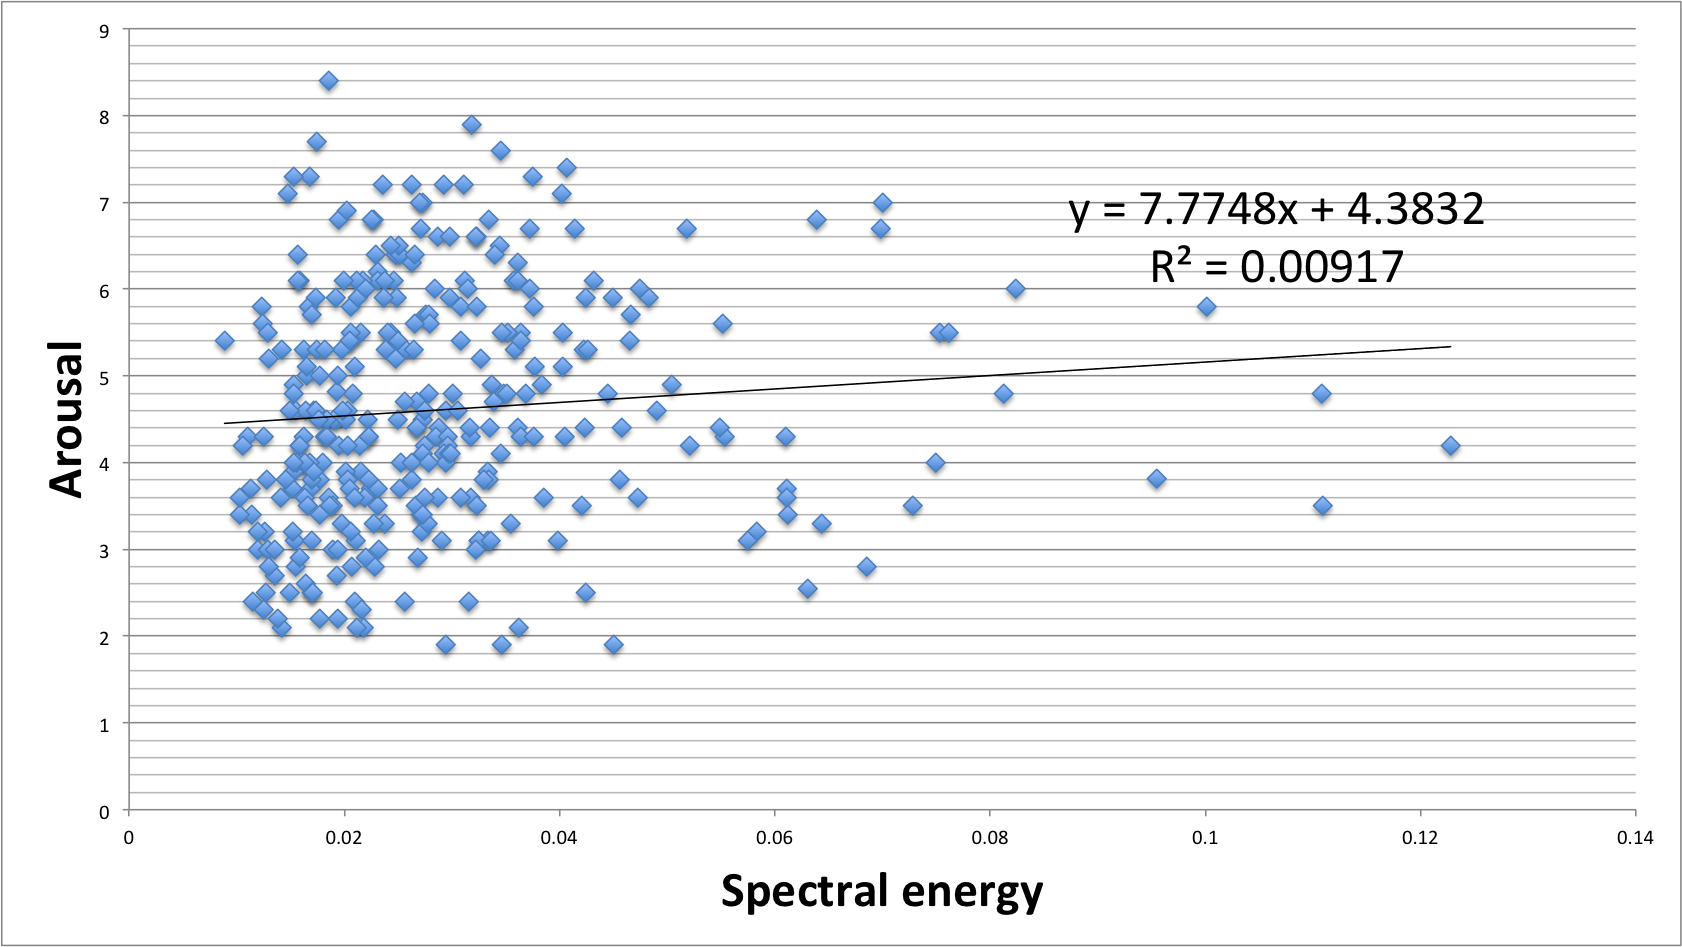
\includegraphics[width=\textwidth]{Figures/spectralenergy-arousal}
			   \vspace{20pt}
        \end{subfigure}
        \begin{subfigure}[b]{0.48\textwidth}
                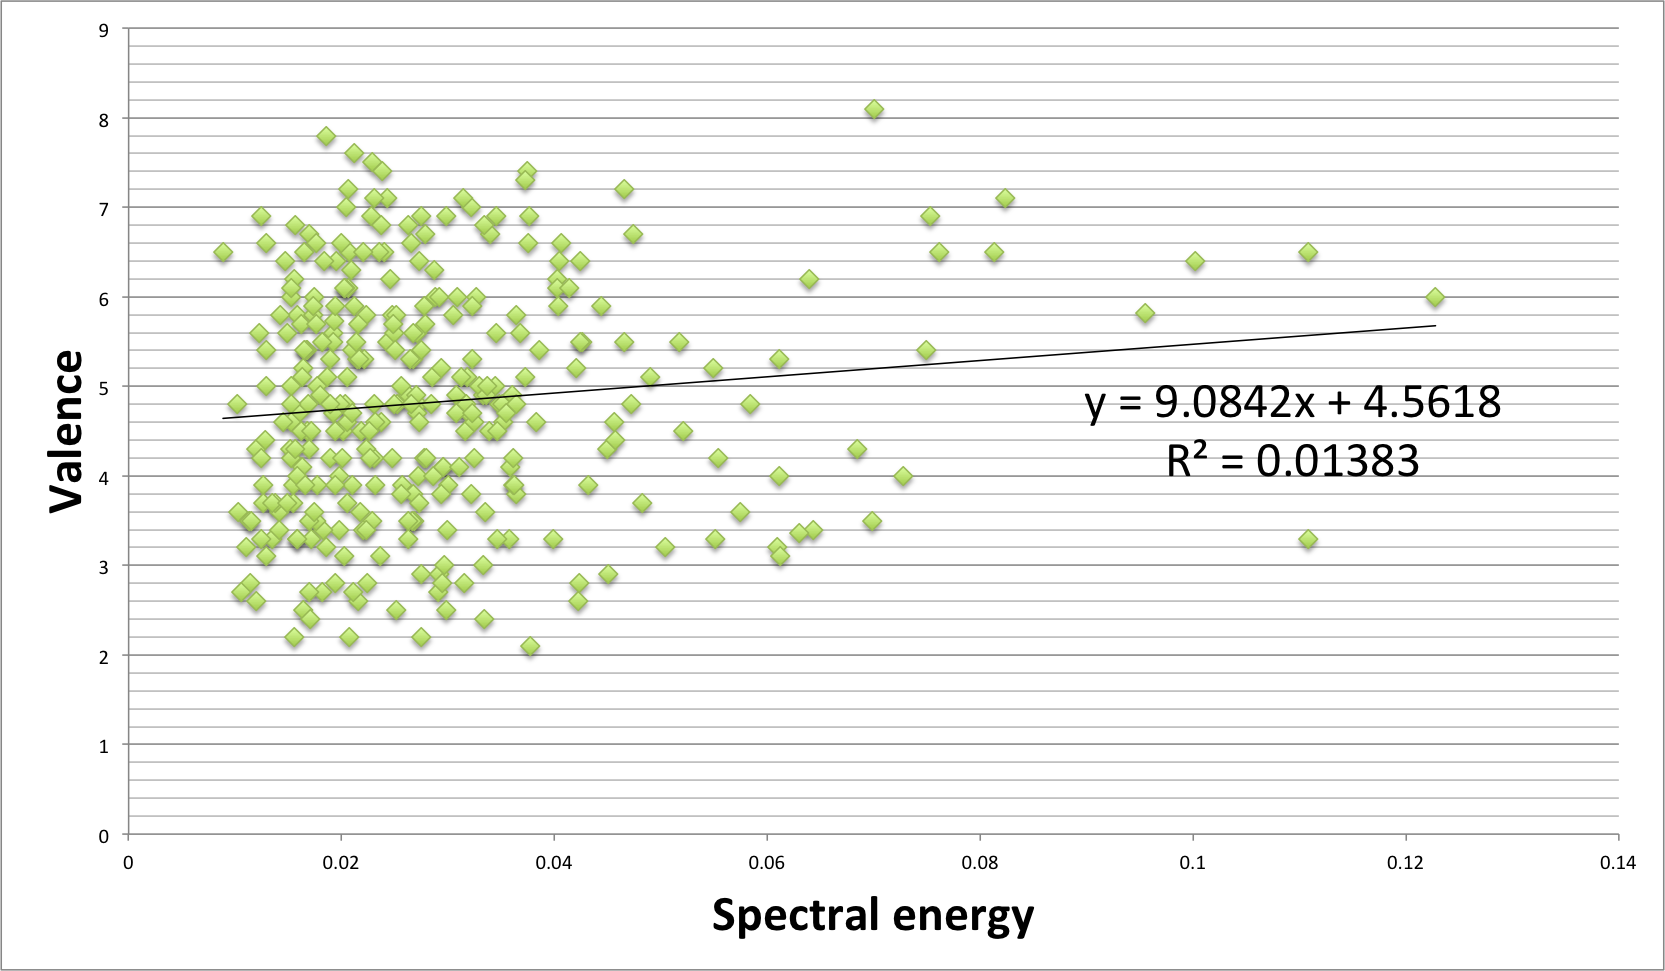
\includegraphics[width=\textwidth]{Figures/spectralenergy-valence}
                  \vspace{20pt}
        \end{subfigure}        
        
        \centering
        \begin{subfigure}[b]{0.48\textwidth}
                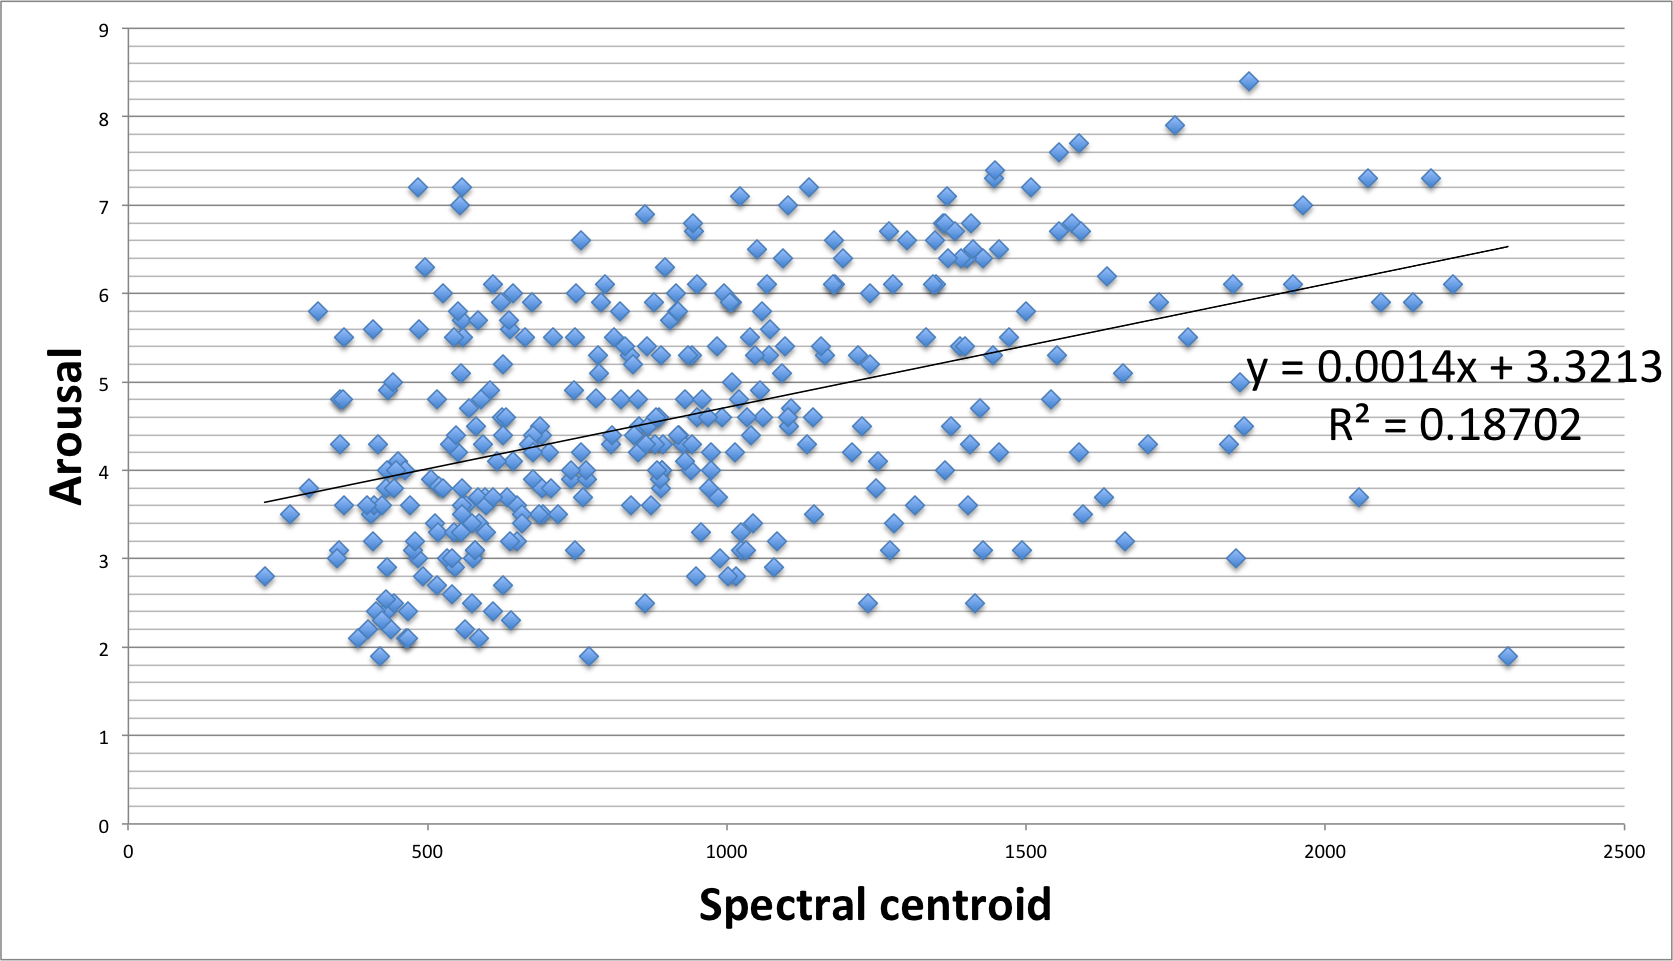
\includegraphics[width=\textwidth]{Figures/spectralcentroid-arousal}
                \vspace{20pt}
        \end{subfigure}
        \begin{subfigure}[b]{0.48\textwidth}
                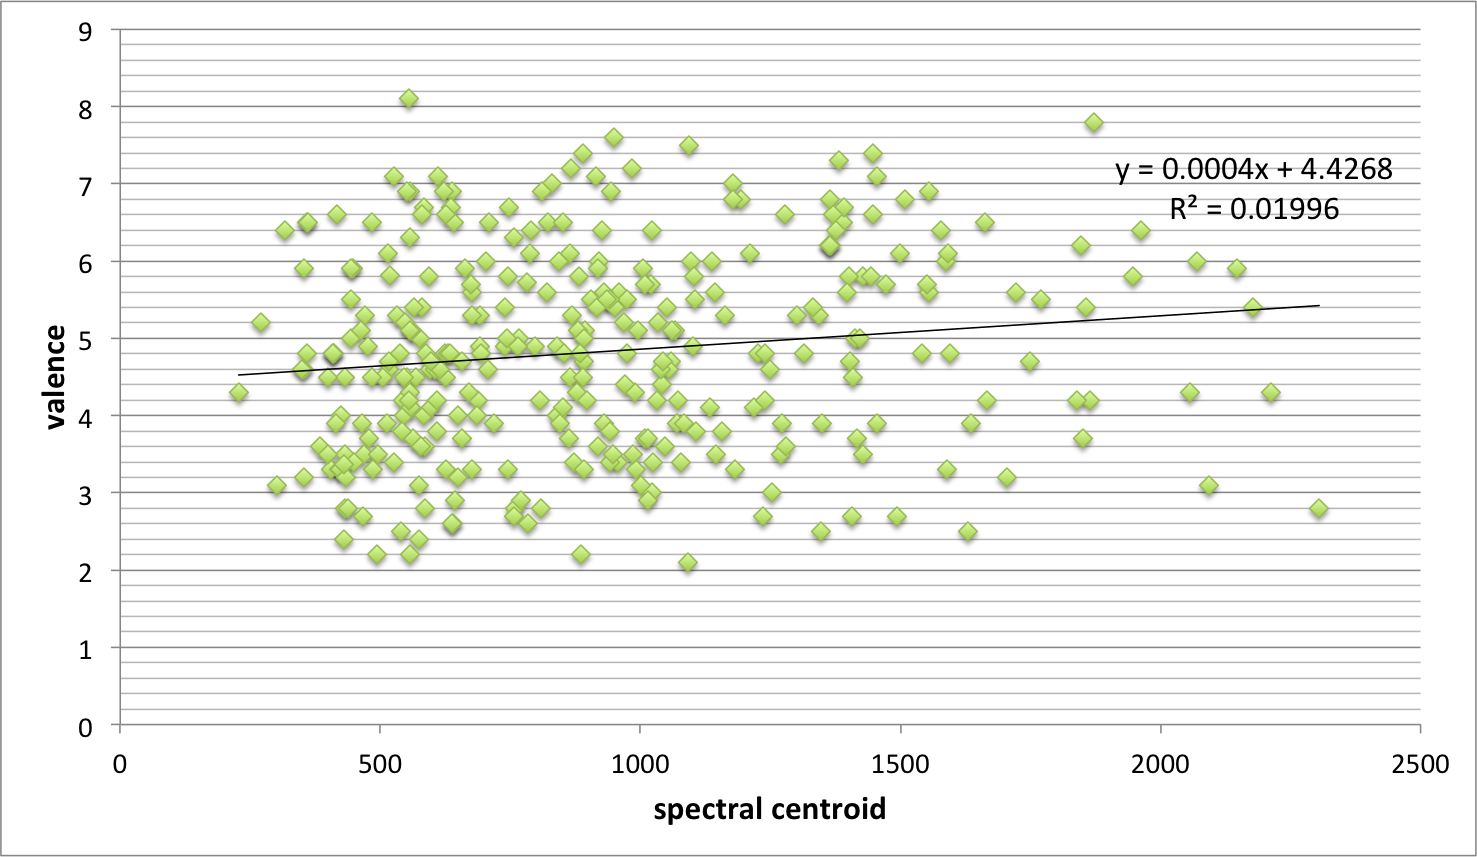
\includegraphics[width=\textwidth]{Figures/spectralcentroid-valence}
                \vspace{20pt}
        \end{subfigure}

\end{figure}
\begin{figure}
 
         \centering
        \begin{subfigure}[b]{0.48\textwidth}
                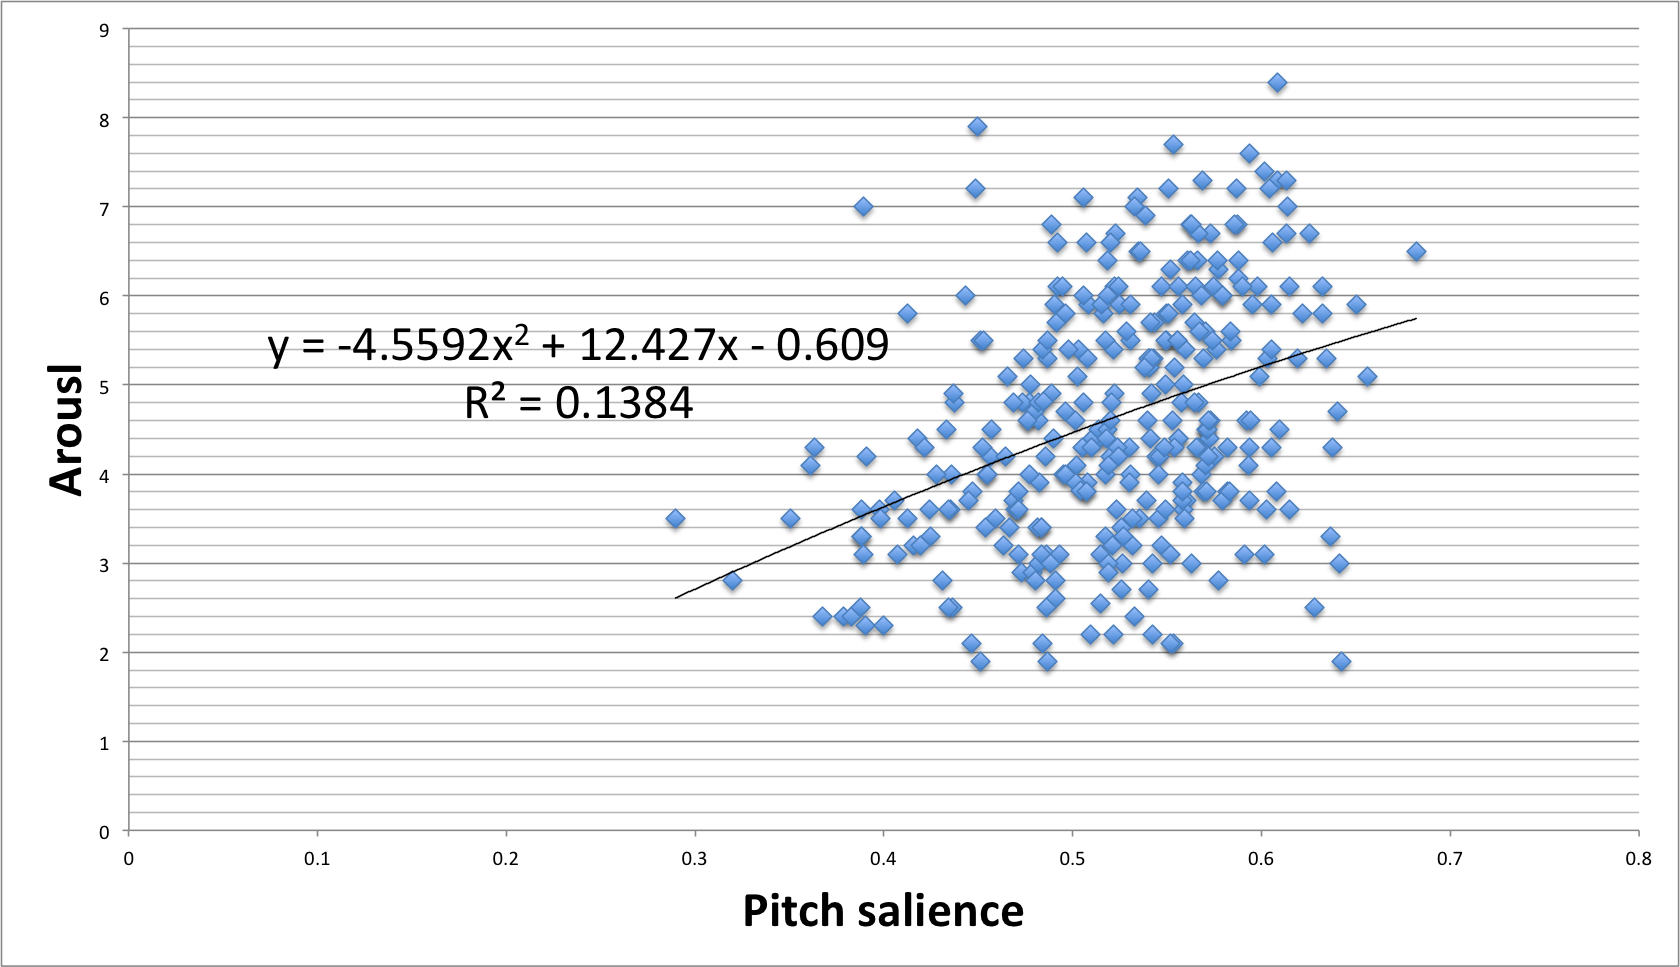
\includegraphics[width=\textwidth]{Figures/pitchsalience-arousal}
			   \vspace{20pt}
        \end{subfigure}
        \begin{subfigure}[b]{0.48\textwidth}
                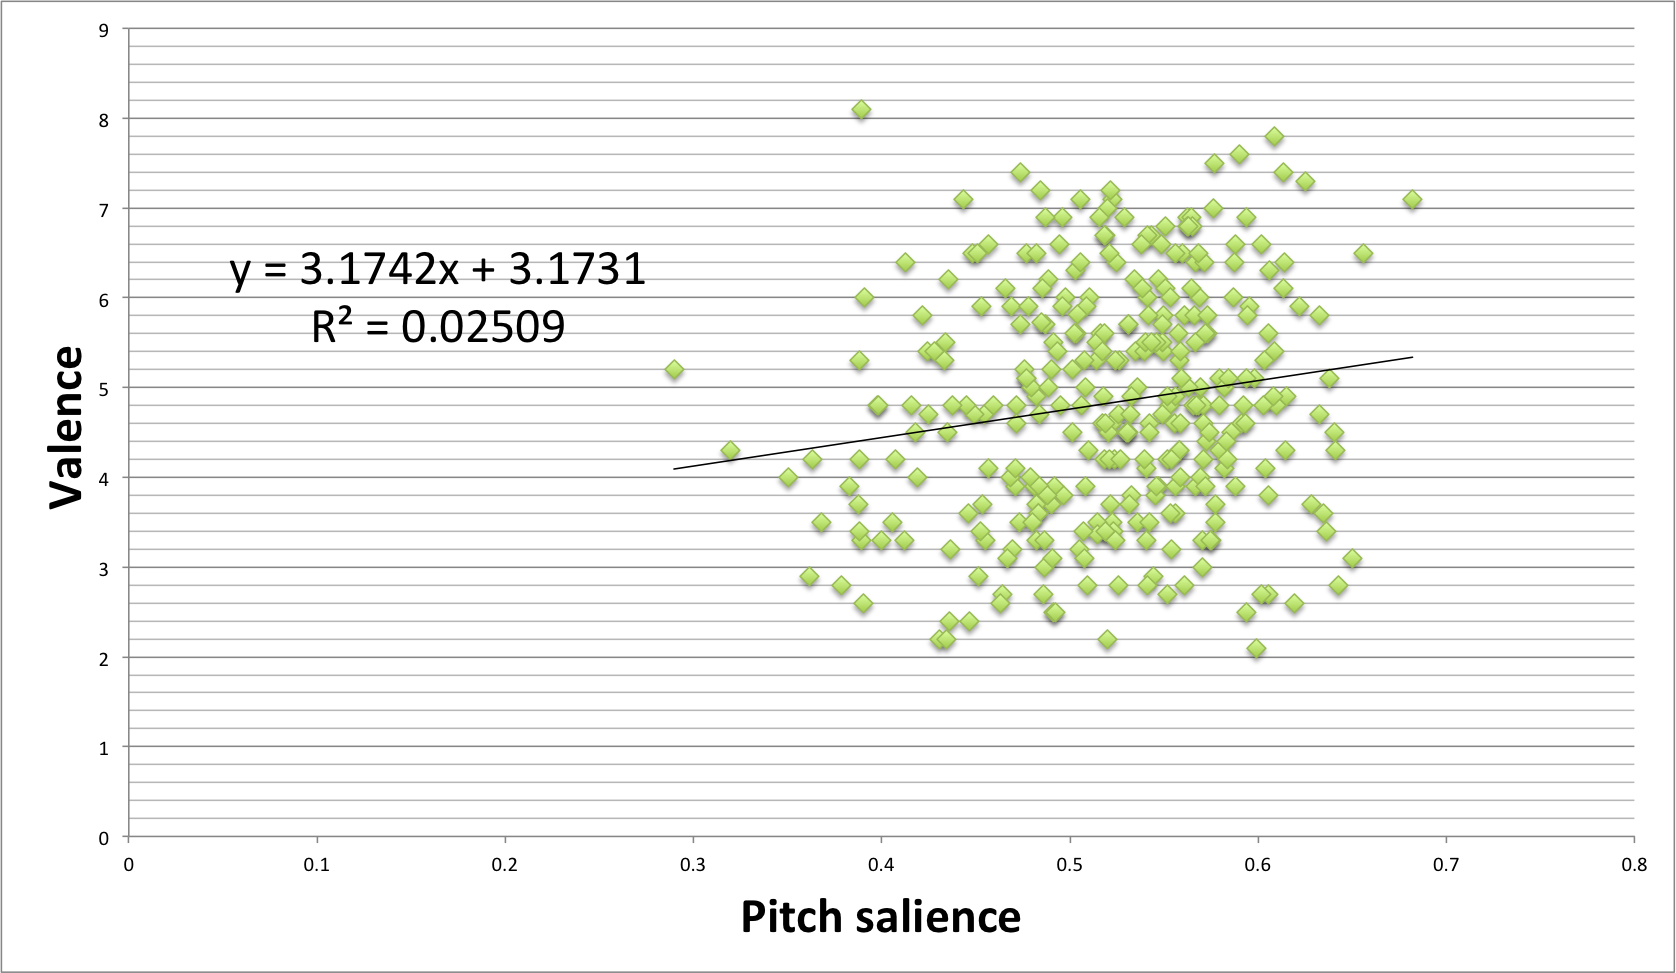
\includegraphics[width=\textwidth]{Figures/pitchsalience-valence}
                  \vspace{20pt}
        \end{subfigure}

          \centering
        \begin{subfigure}[b]{0.48\textwidth}
                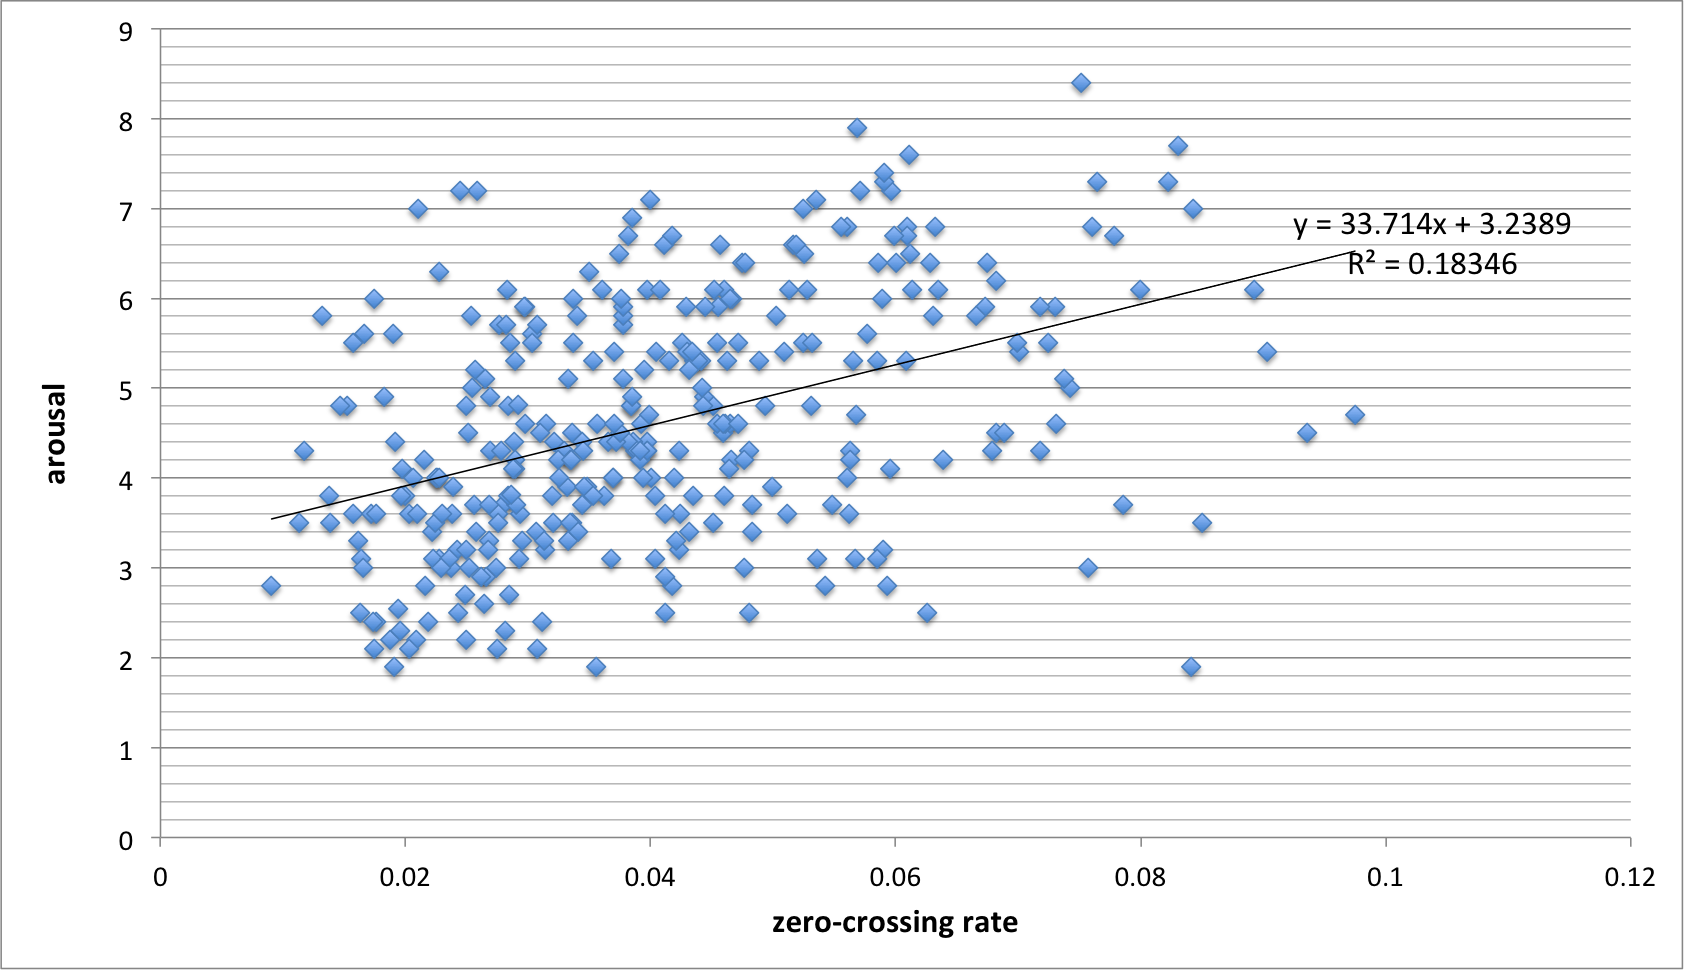
\includegraphics[width=\textwidth]{Figures/zerocrossing-arousal}
			   \vspace{20pt}
        \end{subfigure}
        \begin{subfigure}[b]{0.48\textwidth}
                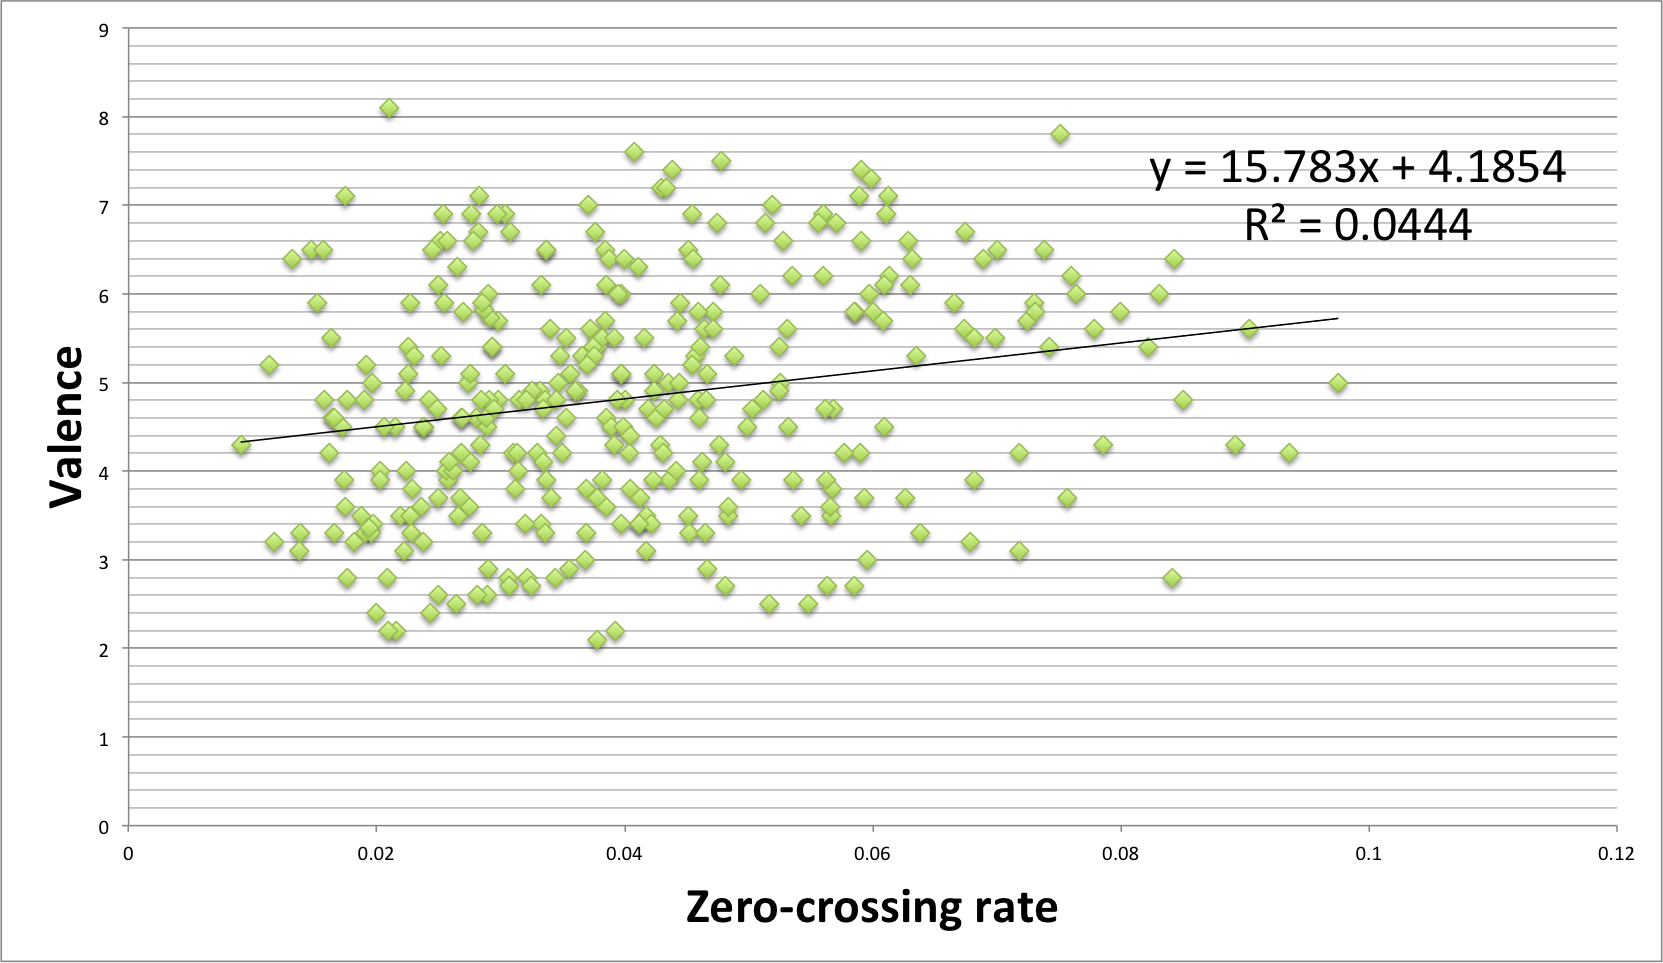
\includegraphics[width=\textwidth]{Figures/zerocrossing-valence}
                  \vspace{20pt}
        \end{subfigure}
        
         \centering
        \begin{subfigure}[b]{0.48\textwidth}
                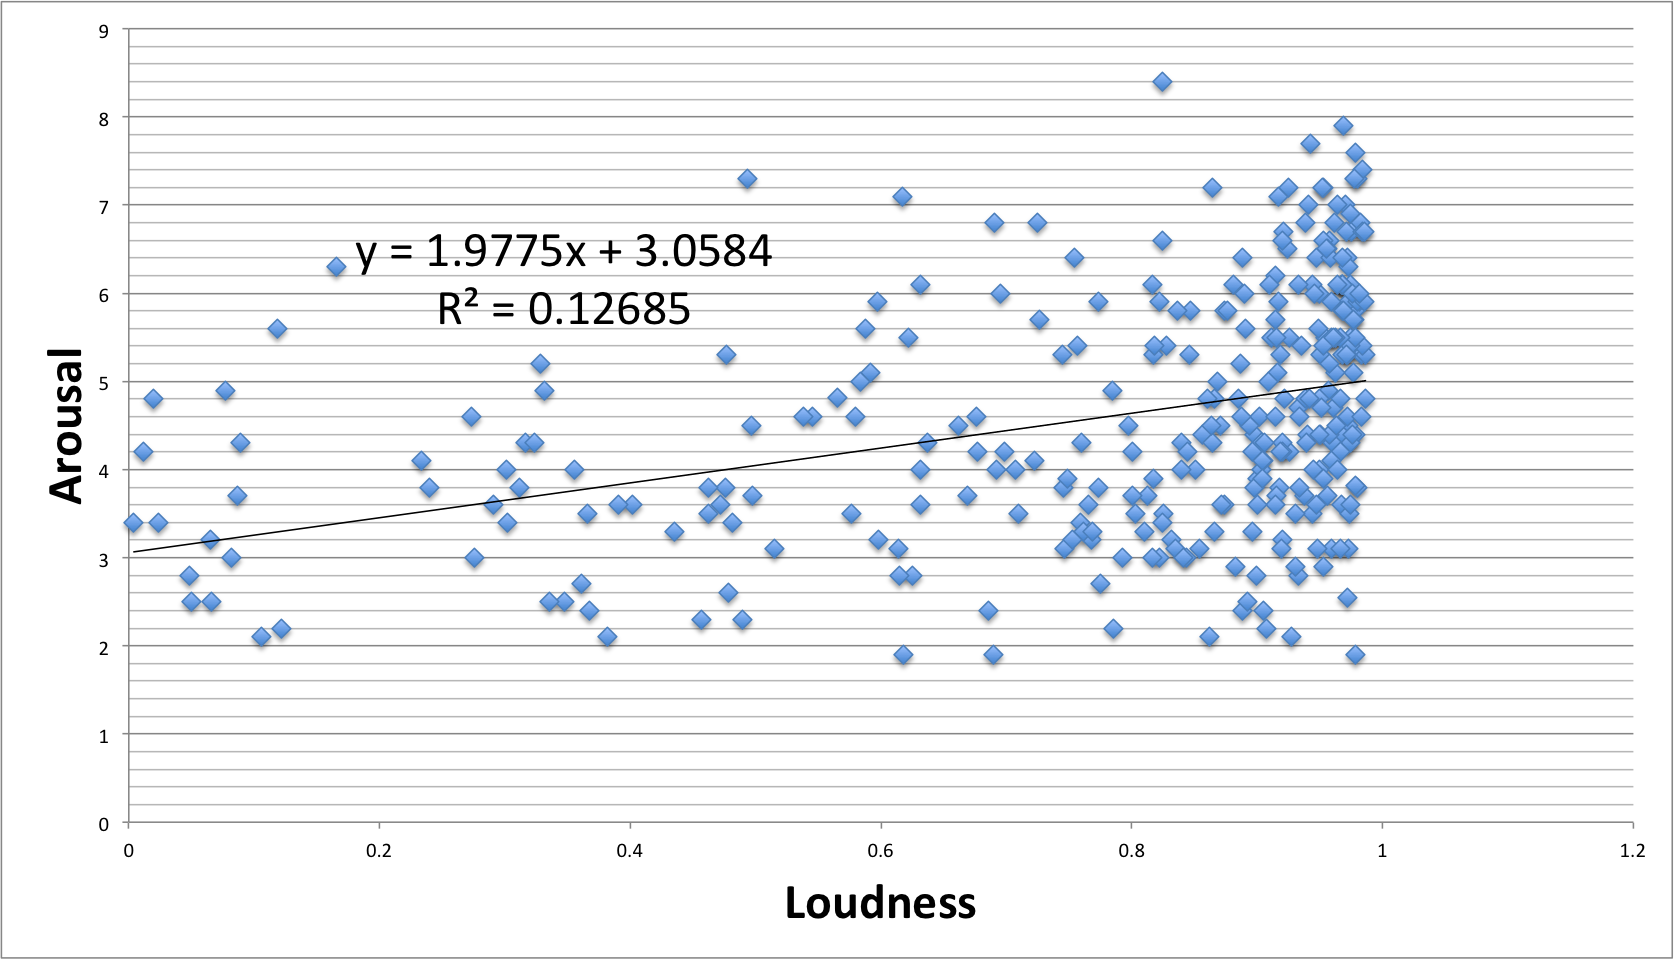
\includegraphics[width=\textwidth]{Figures/loudness-arousal}
			   \vspace{20pt}
        \end{subfigure}
        \begin{subfigure}[b]{0.48\textwidth}
                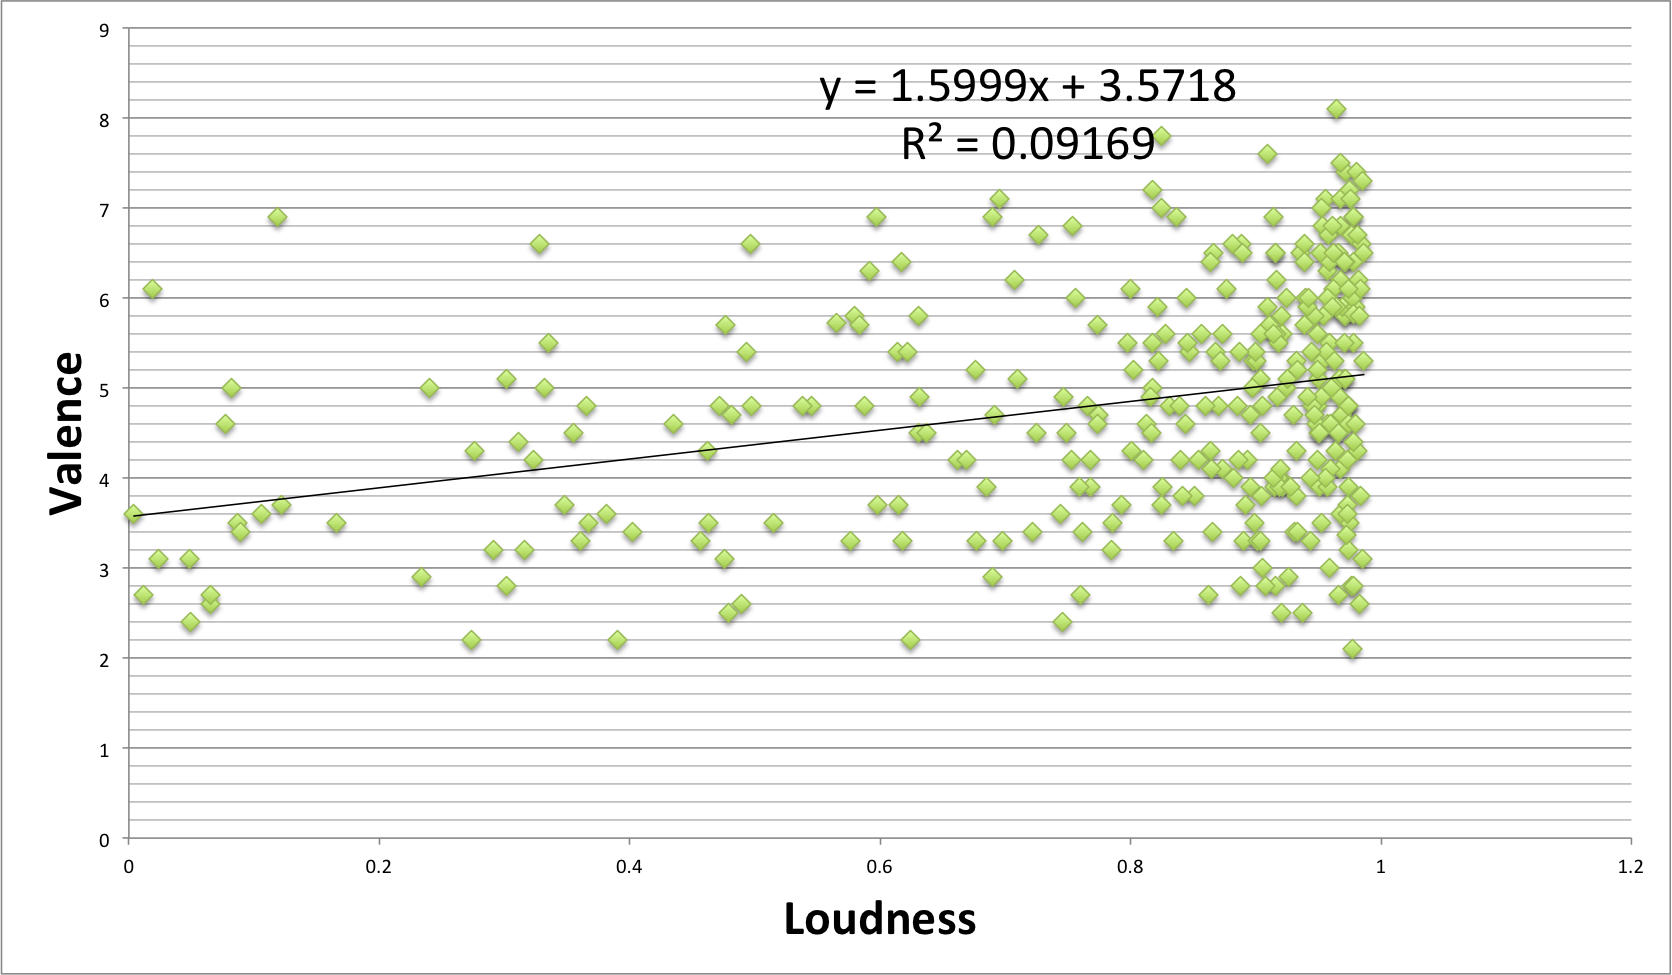
\includegraphics[width=\textwidth]{Figures/loudness-valence}
                  \vspace{20pt}
        \end{subfigure}
        
             \centering
        \begin{subfigure}[b]{0.48\textwidth}
                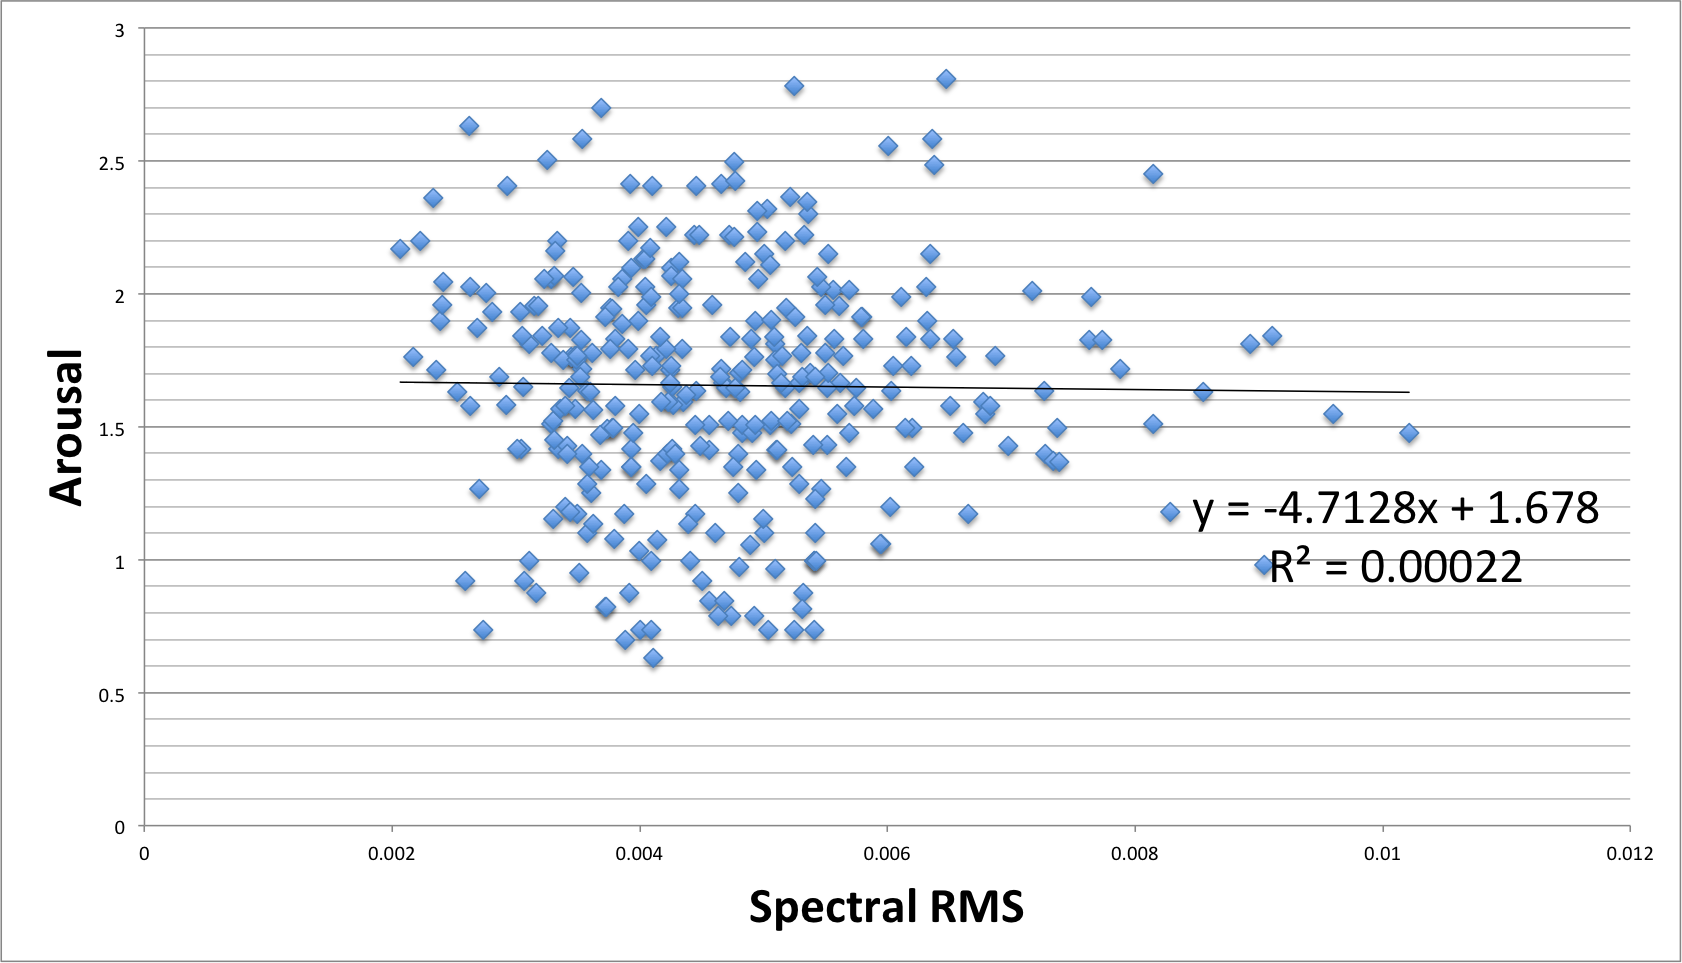
\includegraphics[width=\textwidth]{Figures/spectralrms-arousal}
			   \vspace{20pt}
        \end{subfigure}
        \begin{subfigure}[b]{0.48\textwidth}
                \includegraphics[width=\textwidth]{Figures/spectralrms-valence}
                  \vspace{20pt}
        \end{subfigure}
        
\end{figure}

\begin{figure}  
         \centering
        \begin{subfigure}[b]{0.48\textwidth}
                \includegraphics[width=\textwidth]{Figures/bpm-arousal}
			   \vspace{20pt}
        \end{subfigure}
        \begin{subfigure}[b]{0.48\textwidth}
                \includegraphics[width=\textwidth]{Figures/bpm-valence}
                  \vspace{20pt}
        \end{subfigure}
        
         \centering
        \begin{subfigure}[b]{0.48\textwidth}
                \includegraphics[width=\textwidth]{Figures/silence60mean-arousal}
			   \vspace{20pt}
        \end{subfigure}
        \begin{subfigure}[b]{0.48\textwidth}
                \includegraphics[width=\textwidth]{Figures/silence60mean-valence}
                  \vspace{20pt}
        \end{subfigure}

         \centering
        \begin{subfigure}[b]{0.48\textwidth}
                \includegraphics[width=\textwidth]{Figures/silence60dvar-arousal}
			   \vspace{20pt}
        \end{subfigure}
        \begin{subfigure}[b]{0.48\textwidth}
                \includegraphics[width=\textwidth]{Figures/silence60dvar-valence}
                  \vspace{20pt}
        \end{subfigure}
        
         \centering
        \begin{subfigure}[b]{0.48\textwidth}
                \includegraphics[width=\textwidth]{Figures/dynamiccomplexity-arousal}
			   \vspace{20pt}
        \end{subfigure}
        \begin{subfigure}[b]{0.48\textwidth}
                \includegraphics[width=\textwidth]{Figures/dynamiccomplexity-valence}
                  \vspace{20pt}
        \end{subfigure}
\end{figure}

\begin{figure}
         \centering
        \begin{subfigure}[b]{0.48\textwidth}
                \includegraphics[width=\textwidth]{Figures/silence30mean-arousal}
			   \vspace{20pt}
        \end{subfigure}
        \begin{subfigure}[b]{0.48\textwidth}
                \includegraphics[width=\textwidth]{Figures/silence30mean-valence}
                  \vspace{20pt}
        \end{subfigure}
        
	    \centering
        \begin{subfigure}[b]{0.48\textwidth}
                \includegraphics[width=\textwidth]{Figures/silence30dvar-arousal}
			   \vspace{20pt}
        \end{subfigure}
        \begin{subfigure}[b]{0.48\textwidth}
                \includegraphics[width=\textwidth]{Figures/silence30dvar-valence}
                  \vspace{20pt}
        \end{subfigure}        
        
         \centering
        \begin{subfigure}[b]{0.48\textwidth}
                \includegraphics[width=\textwidth]{Figures/silence20mean-arousal}
			   \vspace{20pt}
        \end{subfigure}
        \begin{subfigure}[b]{0.48\textwidth}
                \includegraphics[width=\textwidth]{Figures/silence20mean-valence}
                  \vspace{20pt}
        \end{subfigure}
        
             \begin{subfigure}[b]{0.48\textwidth}
                \includegraphics[width=\textwidth]{Figures/silence20dvar-arousal}
			   \vspace{20pt}
        \end{subfigure}
        \begin{subfigure}[b]{0.48\textwidth}
                \includegraphics[width=\textwidth]{Figures/silence20dvar-valence}
                  \vspace{20pt}
        \end{subfigure}
        
\end{figure}

\begin{figure}
         \centering
        \begin{subfigure}[b]{0.48\textwidth}
                \includegraphics[width=\textwidth]{Figures/key-arousal}
			   \vspace{20pt}
        \end{subfigure}
        \begin{subfigure}[b]{0.48\textwidth}
                \includegraphics[width=\textwidth]{Figures/key-valence}
                  \vspace{20pt}
        \end{subfigure}
        
	    \centering
        \begin{subfigure}[b]{0.48\textwidth}
                \includegraphics[width=\textwidth]{Figures/keyscale-arousal}
			   \vspace{20pt}
        \end{subfigure}
        \begin{subfigure}[b]{0.48\textwidth}
                \includegraphics[width=\textwidth]{Figures/keyscale-valence}
                  \vspace{20pt}
        \end{subfigure}        
        
         \centering
        \begin{subfigure}[b]{0.48\textwidth}
                \includegraphics[width=\textwidth]{Figures/chordkey-arousal}
			   \vspace{20pt}
        \end{subfigure}
        \begin{subfigure}[b]{0.48\textwidth}
                \includegraphics[width=\textwidth]{Figures/chordkey-valence}
                  \vspace{20pt}
        \end{subfigure}
        
             \begin{subfigure}[b]{0.48\textwidth}
                \includegraphics[width=\textwidth]{Figures/chordscale-arousal}
			   \vspace{20pt}
        \end{subfigure}
        \begin{subfigure}[b]{0.48\textwidth}
                \includegraphics[width=\textwidth]{Figures/chordscale-valence}
                  \vspace{20pt}
        \end{subfigure}
        
\end{figure}

\begin{figure}
         \centering
        \begin{subfigure}[b]{0.48\textwidth}
                \includegraphics[width=\textwidth]{Figures/beatloudnessmean-arousal}
			   \vspace{20pt}
        \end{subfigure}
        \begin{subfigure}[b]{0.48\textwidth}
                \includegraphics[width=\textwidth]{Figures/beatloudnessmean-valence}
                  \vspace{20pt}
        \end{subfigure}
        
	    \centering
        \begin{subfigure}[b]{0.48\textwidth}
                \includegraphics[width=\textwidth]{Figures/beatloudnessdvar-arousal}
			   \vspace{20pt}
        \end{subfigure}
        \begin{subfigure}[b]{0.48\textwidth}
                \includegraphics[width=\textwidth]{Figures/beatloudnessdvar-valence}
                  \vspace{20pt}
        \end{subfigure}        
        
         \centering
        \begin{subfigure}[b]{0.48\textwidth}
                \includegraphics[width=\textwidth]{Figures/dissonancemean-arousal}
			   \vspace{20pt}
        \end{subfigure}
        \begin{subfigure}[b]{0.48\textwidth}
                \includegraphics[width=\textwidth]{Figures/dissonancemean-valence}
                  \vspace{20pt}
        \end{subfigure}
        
	    \centering
        \begin{subfigure}[b]{0.48\textwidth}
                \includegraphics[width=\textwidth]{Figures/dissonancedvar-arousal}
			   \vspace{20pt}
        \end{subfigure}
        \begin{subfigure}[b]{0.48\textwidth}
                \includegraphics[width=\textwidth]{Figures/dissonancedvar-valence}
                  \vspace{20pt}
        \end{subfigure}        
        
\end{figure}
% Appendix Template

\chapter{Appendix B: Structure Retrieval Results} % Main appendix title

\label{AppendixB} % Change X to a consecutive letter; for referencing this appendix elsewhere, use \ref{AppendixB}


\lhead{Appendix B. \emphStructure Retrieval Results} % Change X to a consecutive letter; this is for the header on each page - perhaps a shortened title

\section{Structure Retrieval Results}
\label{sec:mfccappen}

\begin{figure}[b]
    \includegraphics[width=0.75\textwidth]{Figures/mfcc_ssm_euclidean}
    \centering

  \caption{Similarity matrix calculated from Mel-frequency Cepstral Coefficients using Euclidean distance.}
  \label{fig:mfcceuclid}
\end{figure}


\begin{figure}[t]
    \includegraphics[width=0.75\textwidth]{Figures/mfcc_ssm_manhattan}
    \centering

  \caption{Similarity matrix calculated from Mel-frequency Cepstral Coefficients using Manhattan distance.}
  \label{fig:mfccmanhattan}
\end{figure}


\begin{figure}[b]
    \includegraphics[width=0.75\textwidth]{Figures/mfcc_ssm_cosine}
    \centering

  \caption{Similarity matrix calculated from Mel-frequency Cepstral Coefficients using cosine distance.}
  \label{fig:mfcccosine}
\end{figure}


\begin{figure}[b]
    \includegraphics[width=0.75\textwidth]{Figures/mfcc_ssm_synched}
    \centering

  \caption{Similarity matrix calculated from Mel-frequency Cepstral Coefficients using cosine distance.}
  \label{fig:mfcccorrelation}
\end{figure}

%----------------------------------------------------------------------------------------
%	BIBLIOGRAPHY
%----------------------------------------------------------------------------------------

\lhead{\emph{Bibliography}} % Change the page header to say "Bibliography"

\bibliographystyle{unsrtnat} % Use the "unsrtnat" BibTeX style for formatting the Bibliography
\bibliography{Bibliography} % The references (bibliography) information are stored in the file named "Bibliography.bib"


\end{document}  